\documentclass[hyperref, a4paper]{report}

\usepackage{geometry}
\usepackage{titling}
\usepackage{titlesec}
% No longer needed, since we will use enumitem package
% \usepackage{paralist}
\usepackage{enumitem}
\usepackage{footnote}
\usepackage{amsmath, amssymb, amsthm}
\usepackage{mathtools}
\usepackage{bbm}
\usepackage{cite}
\usepackage{graphicx}
\usepackage{subfigure}
\usepackage{simpler-wick}
\usepackage{physics}
\usepackage{tensor}
\usepackage{siunitx}
\usepackage[version=4]{mhchem}
\usepackage{tikz}
\usepackage{xcolor}
\usepackage{listings}
\usepackage{underscore}
\usepackage{autobreak}
\usepackage[ruled, vlined, linesnumbered]{algorithm2e}
\usepackage{nameref,zref-xr}
\zxrsetup{toltxlabel}
\usepackage[colorlinks,unicode]{hyperref} % , linkcolor=black, anchorcolor=black, citecolor=black, urlcolor=black, filecolor=black
\usepackage[most]{tcolorbox}
\usepackage{prettyref}

% Page style
\geometry{left=3.18cm,right=3.18cm,top=2.54cm,bottom=2.54cm}
\titlespacing{\paragraph}{0pt}{1pt}{10pt}[20pt]
\setlength{\droptitle}{-5em}

% More compact lists 
\setlist[itemize]{
    %itemindent=17pt, 
    %leftmargin=1pt,
    listparindent=\parindent,
    parsep=0pt,
}

\setlist[enumerate]{
    %itemindent=17pt, 
    %leftmargin=1pt,
    listparindent=\parindent,
    parsep=0pt,
}

% Math operators
\DeclareMathOperator{\timeorder}{\mathcal{T}}
\DeclareMathOperator{\diag}{diag}
\DeclareMathOperator{\legpoly}{P}
\DeclareMathOperator{\primevalue}{P}
\DeclareMathOperator{\sgn}{sgn}
\DeclareMathOperator{\res}{Res}
\newcommand*{\ii}{\mathrm{i}}
\newcommand*{\ee}{\mathrm{e}}
\newcommand*{\const}{\mathrm{const}}
\newcommand*{\suchthat}{\quad \text{s.t.} \quad}
\newcommand*{\argmin}{\arg\min}
\newcommand*{\argmax}{\arg\max}
\newcommand*{\normalorder}[1]{: #1 :}
\newcommand*{\pair}[1]{\langle #1 \rangle}
\newcommand*{\fd}[1]{\mathcal{D} #1}
\DeclareMathOperator{\bigO}{\mathcal{O}}

% TikZ setting
\usetikzlibrary{arrows,shapes,positioning}
\usetikzlibrary{arrows.meta}
\usetikzlibrary{decorations.markings}
\usetikzlibrary{calc}
\tikzstyle arrowstyle=[scale=1]
\tikzstyle directed=[postaction={decorate,decoration={markings,
    mark=at position .5 with {\arrow[arrowstyle]{stealth}}}}]
\tikzstyle ray=[directed, thick]
\tikzstyle dot=[anchor=base,fill,circle,inner sep=1pt]

% Algorithm setting
% Julia-style code
\SetKwIF{If}{ElseIf}{Else}{if}{}{elseif}{else}{end}
\SetKwFor{For}{for}{}{end}
\SetKwFor{While}{while}{}{end}
\SetKwProg{Function}{function}{}{end}
\SetArgSty{textnormal}

\newcommand*{\concept}[1]{{\textbf{#1}}}

% Embedded codes
\lstset{basicstyle=\ttfamily,
  showstringspaces=false,
  commentstyle=\color{gray},
  keywordstyle=\color{blue}
}

\lstdefinestyle{console}{
    basicstyle=\footnotesize\ttfamily,
    breaklines=true,
    postbreak=\mbox{\textcolor{red}{$\hookrightarrow$}\space}
}

% Reference formatting
\newrefformat{fig}{Figure~\ref{#1}}

% Color boxes
\tcbuselibrary{skins, breakable, theorems}

\newtcbtheorem[number within=chapter]{infobox}{Box}{
    enhanced,
    boxrule=0pt,
    colback=blue!5,
    colframe=blue!5,
    coltitle=blue!50,
    borderline west={4pt}{0pt}{blue!65},
    sharp corners,
    fonttitle=\bfseries, 
    breakable,
    before upper={\parindent15pt\noindent}}{box}
\newtcbtheorem[number within=chapter, use counter from=infobox]{theorybox}{Box}{
    enhanced,
    boxrule=0pt,
    colback=orange!5, 
    colframe=orange!5, 
    coltitle=orange!50,
    borderline west={4pt}{0pt}{orange!65},
    sharp corners,
    fonttitle=\bfseries, 
    breakable,
    before upper={\parindent15pt\noindent}}{box}
\newtcbtheorem[number within=chapter, use counter from=infobox]{learnbox}{Box}{
    enhanced,
    boxrule=0pt,
    colback=green!5,
    colframe=green!5,
    coltitle=green!50,
    borderline west={4pt}{0pt}{green!65},
    sharp corners,
    fonttitle=\bfseries, 
    breakable,
    before upper={\parindent15pt\noindent}}{box}

% Displaying texts in bookmarkers

\pdfstringdefDisableCommands{%
  \def\\{}%
  \def\ce#1{<#1>}%
}

\pdfstringdefDisableCommands{%
  \def\texttt#1{<#1>}%
  \def\mathbb#1{#1}%
}
\pdfstringdefDisableCommands{\def\eqref#1{(\ref{#1})}}

\makeatletter
\pdfstringdefDisableCommands{\let\HyPsd@CatcodeWarning\@gobble}
\makeatother

\newenvironment{shelldisplay}{\begin{lstlisting}}{\end{lstlisting}}

\newcommand{\shortcode}[1]{\texttt{#1}}

\lstset{style = console}

% Make subsubsection labeled
\setcounter{secnumdepth}{4}
\setcounter{tocdepth}{4}

\newcommand*{\abinitio}{\textit{ab initio}}
\newcommand*{\kB}{k_{\text{B}}}
\newcommand*{\epsr}{\epsilon_{\text{r}}}

\title{Manual for DFT+$GW$+BSE and the related matters}
\author{Jinyuan Wu}

\begin{document}
    
\maketitle

\tableofcontents


\chapter{Preliminaries}

\section{Second quantization}

Here are some handy formulae for building second-quantized Hamiltonian 
from wave functions or stuff like that 
that are generated by first-principle softwares.

\subsection{For electrons}

In second quantization, for fermions we have 
\begin{equation}
    \acomm*{c_i}{c_j^\dagger} = \delta_{ij},
\end{equation}
and Fock states are given by
\begin{equation}
    \ket*{n_1, n_2, \ldots} = (c_1^\dagger)^{n_1} (c_2^\dagger)^{n_2} \cdots \ket*{0}.
\end{equation}
This gives us the expected $(-1)$ sign change 
when two fermions are switched. 
A single particle Hamiltonian 
\begin{equation}
    H_0 = \sum_{i=1}^{N} h_i
\end{equation}
is to be rewritten as 
\begin{equation}
    H_0 = \sum_{\alpha, \beta} \mel**{\alpha}{h}{\beta} c_\alpha^\dagger c_\beta,
\end{equation}
and a two-particle Hamiltonian 
\begin{equation}
    H_\text{I} = \frac{1}{2} \sum_{i \neq j = 1}^{N} V_{ij}
    = \sum_{\text{pair $i$, $j$}} V_{ij}
\end{equation}
is to be rewritten as 
\begin{equation}
    H_{\text{I}} = \frac{1}{2} \sum_{\alpha, \beta, \delta, \gamma}
        \mel**{\alpha \beta}{V}{\delta \gamma} 
        c^\dagger_\alpha c^\dagger_\beta c_\delta c_\gamma.
\end{equation}
Note that in the first-quantized Hamiltonian, 
$i$ and $j$ label particles, 
while in the second-quantized Hamiltonian, 
$\alpha, \beta, \delta, \gamma$ label single-particle wave functions.
The $1/2$ factor is there to counter the double counting of $ij$ and $ji$.

The representation switching formulae are 
\begin{equation}
    c_\alpha^\dagger = \sum_{\tilde{\alpha}} \braket*{\tilde{\alpha}}{\alpha} c_{\tilde{\alpha}}^\dagger
\end{equation}
and 
\begin{equation}
    c_\alpha = \sum_{\tilde{\alpha}} \braket*{\alpha}{\tilde{\alpha}} c_{\tilde{\alpha}}.
\end{equation}
Specifically, suppose $\{\alpha\}$ is a single-particle basis, 
we say 
\begin{equation}
    \psi^\dagger(\vb*{x}) = \sum_{\alpha} \braket*{\vb*{x}}{\alpha} c_\alpha^\dagger
\end{equation}
and $\psi(\vb*{x})$ are \concept{field operators}.
Most frequently, $\alpha$ is the momentum (in the Bloch representation) 
or the index of primitive unit cells or atoms (in the Wannier representation).
When $\alpha$ is the momentum, 
the relation between the field operator and the creation operator 
is just Fourier transform.
Usually we just choose the normalization of the field operators to satisfy 
\begin{equation}
    \acomm*{\psi(\vb*{x})}{\psi^\dagger(\vb*{x}')} = \delta(\vb*{x} - \vb*{x}').
\end{equation}
Under this convention, 
if we define 
\begin{equation}
    \psi_{\vb*{k}} = \frac{1}{\sqrt{V}} \ee^{\ii \vb*{k} \cdot \vb*{r}},
\end{equation}
we find 
\begin{equation}
    \acomm*{c_{\vb*{k}_1}}{c^\dagger_{\vb*{k}_2}} = \delta_{\vb*{k}_1 \vb*{k}_2}.
\end{equation}
This convention should be kept in mind in the rest of this note.
A large benefit of this convention 
is it lifts the burden to worry about normalization concerning $\delta$-functions:
no $\delta$-function appears in the rules now!
To carry out Feynman diagrammatic calculations in an actual computer,
a cutoff on the density of $\vb*{k}$ points is needed
(essentially, a cutoff on the size of the system $V$).
This means we should replace $\int \dd[3]{\vb*{k}} / 2\pi $
with properly normalized $\sum_{\vb*{k}}$,
where $\vb*{k}$ goes over the discretely infinite $\vb*{k}$-grid.

\section{Details in diagrammatics}\label{sec:details-in-diagram}

This section briefly goes through some tricky aspects of Feynman diagram techniques 
that may seem puzzling when we do concrete calculations.

\subsection{Infinitesimals}\label{sec:cond.infinitesimal}

There are some infinitesimals in Feynman rules that are often ignored.
The first is about the illdefinedness
of $\timeorder \expval*{c(t) c^\dagger(0)}$ 
when $t = 0$.
We want to make the propagator to be the particle number 
(so that if we evaluate the tadpole diagram, 
we get the Hartree term). 
Therefore, the contribution of an electron line is  
\begin{equation}
    \begin{aligned}
        \begin{gathered}
            \begin{tikzpicture}[x=0.75pt,y=0.75pt,yscale=-1,xscale=1, baseline=(XXXX.south) ]
                \path (0,48);\path (95.33333587646484,0);\draw    ($(current bounding box.center)+(0,0.3em)$) node [anchor=south] (XXXX) {};
                %Straight Lines [id:da8873009977937396] 
                \draw    (18.53,25) -- (75.83,25) ;
                \draw [shift={(50.98,25)}, rotate = 180] [fill={rgb, 255:red, 0; green, 0; blue, 0 }  ][line width=0.08]  [draw opacity=0] (8.93,-4.29) -- (0,0) -- (8.93,4.29) -- (5.93,0) -- cycle    ;
                % Text Node
                \draw (47.18,26.7) node [anchor=north] [inner sep=0.75pt]    {$k$};
            \end{tikzpicture}
        \end{gathered}
        &\coloneqq 
        \timeorder \expval*{c_{\vb*{k}}(t - 0^+) c_{\vb*{k}}^\dagger(0)}  \\
        &= \int \frac{\dd{\omega}}{2\pi} \ee^{- \ii \omega (t - 0^+)} 
        \underbrace{
            \frac{\ii}{\omega - \xi_{\vb*{k}} + \ii 0^+ \sgn(\xi_{\vb*{k}})}
        }_{\ii G_0(\omega, \vb*{k})}
        = \int \frac{\dd{\omega}}{2\pi} \ee^{- \ii \omega t} \ee^{\ii \omega 0^+} \ii G_0(\omega, \vb*{k}) .
    \end{aligned} 
    \label{eq:green-time-delay}
\end{equation}
In the notation used here, 
$G(t, 0)$ is proportional to $\timeorder \expval*{c(t) c^\dagger(0)}$
and therefore is not well-defined when $t = 0$; 
the infinitesimal therefore is introduced explicitly by 
adding the $\ee^{\ii \omega 0^+}$ factor;
some may \emph{define} that $\ii G$ is the correct propagator,
and the $\ee^{\ii \omega 0^+}$ factor or the small time displacement 
is embedded into the definition of $G$.

The necessity of this $\ee^{\ii \omega 0^+}$ factor 
can also be seen by explicitly doing the integration:
when $t = 0$, if we ignore the $\ee^{\ii \omega 0^+}$ factor, 
we get 
\[
    \int \frac{\dd{\omega}}{2\pi} \frac{\ii}{ \omega - \xi_{\vb*{k}} + \ii 0^+ \sgn(\xi_{\vb*{k}})}.
\]
This integral is not zero, but we want it to be zero when $\xi_{\vb*{k}} > 0$,
so we have to add a $\ee^{\ii \omega 0^+}$ factor
to make the integrand approaches zero quickly enough in the upper plane,
so we can construct an integration contour in the upper plane,
in which there is no pole, 
and 
\[
    \int_{\abs{\omega} = R \gg 1} \ee^{\ii \omega 0^+} \frac{\dd{\omega}}{2\pi} 
    \frac{\ii}{ \omega - \xi_{\vb*{k}} + \ii 0^+ \sgn(\xi_{\vb*{k}})} = 0.
\]

Note that an interaction line should also receive the same mini-regularization 
outlined for Green functions, 
because it's obtained by integrating out some intermediate states. 
For bare Coulomb interaction this is not needed,
because we don't have $\omega$ dependence in the potential,
and it makes no sense to discuss the poles when we change $\omega$.
It does make sense to talk about retardation 
in the relativistic origin of Coulomb interaction:
the Coulomb interaction is mediated by virtual photons,
and is therefore proportional to the off-shell (i.e. $\omega \to 0$) limit of 
the photon propagator, 
which has $\omega^2 - \vb*{q}^2 + \ii 0^+$ 
as the denominator, and we get 
\begin{equation}
    V(q) = \frac{4\pi e^2}{\vb*{q}^2 - \omega^2 - \ii 0^+}.
    \label{eq:v-light-rel}
\end{equation}
Also, for screened Coulomb interaction, 
the correct retardation is important,
because now something looking like \eqref{eq:v-light-rel} appears again.

The $1^+$ in $\Sigma(1, 2) = \ii W(1^+, 2) G(1, 2)$ 
seems to be from the infinitesimal in the electronic Green function 
instead of the infinitesimal in the Coulomb interaction line
(\prettyref{sec:gw-bse.overview-gw.infinitesimal}).

\subsection{The expression of $\Sigma$ and $W$}\label{sec:gw-bse.preliminaries.diagram.corrections}

In this section I only consider how many imaginary units there are in front of 
Green functions, self energies, etc.
Normalization factors like $2\pi$ or $V$ 
involved in summation of $\vb*{r}$ or $\vb*{k}$ are not considered.

The self-energy correction is visualized as the follows:
\begin{equation}
    - \Sigma^{\text{Hartree}}_{\vb*{k} \sigma \omega} = \begin{gathered}
        \begin{tikzpicture}[x=0.75pt,y=0.75pt,yscale=-1,xscale=1]
            %uncomment if require: \path (0,300); %set diagram left start at 0, and has height of 300
            
            %Straight Lines [id:da7796585827567135] 
            \draw  [dash pattern={on 4.5pt off 4.5pt}]  (247.35,162.98) -- (247.35,211) ;
            %Shape: Circle [id:dp5603225998122126] 
            \draw   (218.35,133.98) .. controls (218.35,117.96) and (231.34,104.98) .. (247.35,104.98) .. controls (263.37,104.98) and (276.35,117.96) .. (276.35,133.98) .. controls (276.35,150) and (263.37,162.98) .. (247.35,162.98) .. controls (231.34,162.98) and (218.35,150) .. (218.35,133.98) -- cycle ;
            %Straight Lines [id:da24340217870718206] 
            \draw    (254.35,105.98) ;
            \draw [shift={(254.35,105.98)}, rotate = 180] [fill={rgb, 255:red, 0; green, 0; blue, 0 }  ][line width=0.08]  [draw opacity=0] (12,-3) -- (0,0) -- (12,3) -- cycle    ;
            
            % Text Node
            \draw (217,83.4) node [anchor=north west][inner sep=0.75pt]    {$\boldsymbol{k} ',\alpha ,0$};
            \end{tikzpicture}      
   \end{gathered} = \frac{1}{V} \sum_{\vb*{k}', \alpha} (- V_0) n_{\vb*{k}' \alpha}^0,
   \label{eq:lowerest-self-energy-hartree-fermi-liquid}
\end{equation}
and from it we have 
\[
    \ii G= \ii G_{0} + \ii G_{0} \ii G\times \tikzset{every picture/.style={line width=0.75pt}} %set default line width to 0.75pt        
\begin{tikzpicture}[x=0.75pt,y=0.75pt,yscale=-1,xscale=1, baseline=(XXXX.south) ]
\path (0,75);\path (56,0);\draw    ($(current bounding box.center)+(0,0.3em)$) node [anchor=south] (XXXX) {};
%Shape: Circle [id:dp046942194255674474] 
\draw  [fill={rgb, 255:red, 155; green, 155; blue, 155 }  ,fill opacity=1 ] (8.54,37.54) .. controls (8.54,27.35) and (16.81,19.08) .. (27,19.08) .. controls (37.19,19.08) and (45.46,27.35) .. (45.46,37.54) .. controls (45.46,47.74) and (37.19,56) .. (27,56) .. controls (16.81,56) and (8.54,47.74) .. (8.54,37.54) -- cycle ;
\end{tikzpicture}.
\]
It's then a good idea to define 
\begin{equation}
    -\ii \Sigma =\tikzset{every picture/.style={line width=0.75pt}} %set default line width to 0.75pt        
    \begin{tikzpicture}[x=0.75pt,y=0.75pt,yscale=-1,xscale=1, baseline=(XXXX.south) ]
    \path (0,75);\path (56,0);\draw    ($(current bounding box.center)+(0,0.3em)$) node [anchor=south] (XXXX) {};
    %Shape: Circle [id:dp046942194255674474] 
    \draw  [fill={rgb, 255:red, 155; green, 155; blue, 155 }  ,fill opacity=1 ] (8.54,37.54) .. controls (8.54,27.35) and (16.81,19.08) .. (27,19.08) .. controls (37.19,19.08) and (45.46,27.35) .. (45.46,37.54) .. controls (45.46,47.74) and (37.19,56) .. (27,56) .. controls (16.81,56) and (8.54,47.74) .. (8.54,37.54) -- cycle ;
    \end{tikzpicture},
    \label{eq:sigma-diagram}
\end{equation}
because in this case, we have 
\begin{equation}
    G = G_0 + G G_0 \Sigma,
    \label{eq:dyson-green}
\end{equation}
and therefore 
\begin{equation}
    \underbrace{\omega - \xi^0_{\vb*{k}}}_{{1}/{G_0}} = \underbrace{\omega - \xi_{\vb*{k}}}_{1 / G} + \Sigma,
\end{equation}
which agrees with the definition of the self energy as the shift of single-particle energy from the free dispersion.

It should be noted that the derivations above are 
mainly about how to set the position of $\ii$ correctly:
I left the $\ee^{\ii \omega 0^+}$ factor (which can be found in \eqref{eq:green-time-delay}) out.
After taking these factors into account, 
we find \eqref{eq:dyson-green} becomes 
\begin{equation}
    \ee^{\ii \omega 0^+} \ii G =  
    \ee^{\ii \omega 0^+} \ii G_0 + 
    \ee^{\ii \omega 0^+} \ii G_0 \times
    \begin{tikzpicture}[x=0.75pt,y=0.75pt,yscale=-1,xscale=1, baseline=(XXXX.south) ]
        \path (0,75);\path (56,0);\draw    ($(current bounding box.center)+(0,0.3em)$) node [anchor=south] (XXXX) {};
        %Shape: Circle [id:dp046942194255674474] 
        \draw  [fill={rgb, 255:red, 155; green, 155; blue, 155 }  ,fill opacity=1 ] (8.54,37.54) .. controls (8.54,27.35) and (16.81,19.08) .. (27,19.08) .. controls (37.19,19.08) and (45.46,27.35) .. (45.46,37.54) .. controls (45.46,47.74) and (37.19,56) .. (27,56) .. controls (16.81,56) and (8.54,47.74) .. (8.54,37.54) -- cycle ;
    \end{tikzpicture}
    \times \ee^{\ii \omega 0^+} \ii G.
\end{equation}
We can eliminate the common $\ii \ee^{\ii \omega 0^+}$ factor
(note that the magnitude of $0^+$ doesn't matter, 
so a finite product of $\ee^{\ii \omega 0^+}$ collapses into a single $\ee^{\ii \omega 0^+}$),
and thus we get \eqref{eq:sigma-diagram} again;
but note that for the same ``collapse of finite product of $\ee^{\ii \omega 0^+}$'' reason outlined above, 
the $\ee^{\ii \omega 0^+}$ factor in the RHS of \eqref{eq:sigma-diagram},
if any, can also be removed. 

Similarly, we define the corrected interaction line as 
\begin{equation}
    -\ii W=\tikzset{every picture/.style={line width=0.75pt}} %set default line width to 0.75pt        
    \begin{tikzpicture}[x=0.75pt,y=0.75pt,yscale=-1,xscale=1, baseline=(XXXX.south) ]
    \path (0,75);\path (32,0);\draw    ($(current bounding box.center)+(0,0.3em)$) node [anchor=south] (XXXX) {};
    %Straight Lines [id:da583204631520762] 
    \draw    (14.5,62.99) .. controls (12.85,61.3) and (12.87,59.64) .. (14.55,57.99) .. controls (16.23,56.34) and (16.24,54.67) .. (14.59,52.99) .. controls (12.94,51.31) and (12.96,49.64) .. (14.64,47.99) .. controls (16.32,46.34) and (16.33,44.67) .. (14.68,42.99) .. controls (13.03,41.31) and (13.05,39.64) .. (14.73,37.99) .. controls (16.41,36.34) and (16.43,34.67) .. (14.78,32.99) .. controls (13.13,31.31) and (13.14,29.64) .. (14.82,27.99) .. controls (16.5,26.34) and (16.52,24.67) .. (14.87,22.99) .. controls (13.22,21.31) and (13.24,19.64) .. (14.92,17.99) -- (14.94,15.59) -- (14.94,15.59)(17.5,63.01) .. controls (15.85,61.33) and (15.87,59.66) .. (17.55,58.01) .. controls (19.23,56.36) and (19.24,54.69) .. (17.59,53.01) .. controls (15.94,51.33) and (15.96,49.66) .. (17.64,48.01) .. controls (19.32,46.36) and (19.33,44.69) .. (17.68,43.01) .. controls (16.03,41.33) and (16.05,39.66) .. (17.73,38.01) .. controls (19.41,36.36) and (19.43,34.7) .. (17.78,33.02) .. controls (16.13,31.34) and (16.14,29.67) .. (17.82,28.02) .. controls (19.5,26.37) and (19.52,24.7) .. (17.87,23.02) .. controls (16.22,21.34) and (16.24,19.67) .. (17.92,18.02) -- (17.94,15.62) -- (17.94,15.62) ;
    \end{tikzpicture},
\end{equation}
because in this way, when there is no interaction corrections,
we have 
\begin{equation}
    W = \frac{e^2}{r} \eqqcolon v.
\end{equation}

\subsection{About ``antiparticles''}

The directions of momentum lines indicate whether the particles are created or annihilated.
When the momentum arrow goes against the arrow on a line,
we say this line is an antiparticle line.
But here is a puzzle:
we know there is no such thing as positrons in condensed matter physics,
so what does ``antiparticle'' mean?

Here the problem lies on what it means to be the antiparticle of a kind of particle.
In particle physics,
when we do the particle-antiparticle transformation to an electron state 
whose polarization is one of the Dirac basis,
a $\psi^+$ particle is flipped into a $\psi^-$ particle and vice versa.
In condensed matter physics, the label of $\psi^+$ and $\psi^-$
(or $\phi$ and $\chi$ as people often call them:
$\psi = (\phi, \chi)$) is no longer there:
the $\chi$ modes in the Dirac field have already been integrated out.
So electrons in condensed matter physics don't really have antiparticles 
in the context of high energy physics.

Indeed, if we are still dealing with scattering problems in the non-relativistic limit,
the antiparticle lines don't appear at all!
And similar to the case in QED (which can be checked in Peskin (A.6)), 
no separate momentum arrows parallel to the internal lines are needed:
When calculating the propagator, 
the processes of both ``an electron traveling forward'' and ``a hole traveling backward''
are automatically covered together.

The antiparticle lines only appear when there are electrons in the ground state,
which usually indicates there is a $-\mu N$ term in the Hamiltonian
so having some preexisting electrons lower the energy further,
and this differs with the scattering case only in the rules pertaining to the external lines.
For external lines, we now have diagrams like the following:
\[
\begin{gathered}
    \begin{tikzpicture}[x=0.75pt,y=0.75pt,yscale=-0.8,xscale=0.8]
        %uncomment if require: \path (0,300); %set diagram left start at 0, and has height of 300
        
        %Straight Lines [id:da22337196735465925] 
        \draw    (59,160) .. controls (60.67,158.33) and (62.33,158.33) .. (64,160) .. controls (65.67,161.67) and (67.33,161.67) .. (69,160) .. controls (70.67,158.33) and (72.33,158.33) .. (74,160) .. controls (75.67,161.67) and (77.33,161.67) .. (79,160) .. controls (80.67,158.33) and (82.33,158.33) .. (84,160) .. controls (85.67,161.67) and (87.33,161.67) .. (89,160) .. controls (90.67,158.33) and (92.33,158.33) .. (94,160) .. controls (95.67,161.67) and (97.33,161.67) .. (99,160) .. controls (100.67,158.33) and (102.33,158.33) .. (104,160) .. controls (105.67,161.67) and (107.33,161.67) .. (109,160) -- (112,160) -- (112,160) ;
        %Straight Lines [id:da2810352455475442] 
        \draw    (112,160) -- (154,115.21) ;
        \draw [shift={(137.79,132.5)}, rotate = 133.16] [fill={rgb, 255:red, 0; green, 0; blue, 0 }  ][line width=0.08]  [draw opacity=0] (12,-3) -- (0,0) -- (12,3) -- cycle    ;
        %Straight Lines [id:da3072568651468959] 
        \draw    (154,206.21) -- (112,160) ;
        \draw [shift={(128.29,177.92)}, rotate = 47.73] [fill={rgb, 255:red, 0; green, 0; blue, 0 }  ][line width=0.08]  [draw opacity=0] (12,-3) -- (0,0) -- (12,3) -- cycle    ;
        %Straight Lines [id:da8519748557010314] 
        \draw    (111,146) -- (135.61,120.64) ;
        \draw [shift={(137,119.21)}, rotate = 134.14] [fill={rgb, 255:red, 0; green, 0; blue, 0 }  ][line width=0.08]  [draw opacity=0] (12,-3) -- (0,0) -- (12,3) -- cycle    ;
        %Straight Lines [id:da18850975613378163] 
        \draw    (111,173) -- (133.65,197.73) ;
        \draw [shift={(135,199.21)}, rotate = 227.52] [fill={rgb, 255:red, 0; green, 0; blue, 0 }  ][line width=0.08]  [draw opacity=0] (12,-3) -- (0,0) -- (12,3) -- cycle    ;
        %Straight Lines [id:da6750821989366331] 
        \draw    (214,160) .. controls (215.67,158.33) and (217.33,158.33) .. (219,160) .. controls (220.67,161.67) and (222.33,161.67) .. (224,160) .. controls (225.67,158.33) and (227.33,158.33) .. (229,160) .. controls (230.67,161.67) and (232.33,161.67) .. (234,160) .. controls (235.67,158.33) and (237.33,158.33) .. (239,160) .. controls (240.67,161.67) and (242.33,161.67) .. (244,160) .. controls (245.67,158.33) and (247.33,158.33) .. (249,160) .. controls (250.67,161.67) and (252.33,161.67) .. (254,160) .. controls (255.67,158.33) and (257.33,158.33) .. (259,160) .. controls (260.67,161.67) and (262.33,161.67) .. (264,160) -- (267,160) -- (267,160) ;
        %Straight Lines [id:da7852623112527173] 
        \draw    (267,160) -- (309,115.21) ;
        \draw [shift={(292.79,132.5)}, rotate = 133.16] [fill={rgb, 255:red, 0; green, 0; blue, 0 }  ][line width=0.08]  [draw opacity=0] (12,-3) -- (0,0) -- (12,3) -- cycle    ;
        %Straight Lines [id:da940793106803989] 
        \draw    (309,206.21) -- (267,160) ;
        \draw [shift={(283.29,177.92)}, rotate = 47.73] [fill={rgb, 255:red, 0; green, 0; blue, 0 }  ][line width=0.08]  [draw opacity=0] (12,-3) -- (0,0) -- (12,3) -- cycle    ;
        %Straight Lines [id:da5232058447471666] 
        \draw    (266,146) -- (290.61,120.64) ;
        \draw [shift={(292,119.21)}, rotate = 134.14] [fill={rgb, 255:red, 0; green, 0; blue, 0 }  ][line width=0.08]  [draw opacity=0] (12,-3) -- (0,0) -- (12,3) -- cycle    ;
        %Straight Lines [id:da3253102481261483] 
        \draw    (267.35,174.47) -- (290,199.21) ;
        \draw [shift={(266,173)}, rotate = 47.52] [fill={rgb, 255:red, 0; green, 0; blue, 0 }  ][line width=0.08]  [draw opacity=0] (12,-3) -- (0,0) -- (12,3) -- cycle    ;
        \end{tikzpicture}
\end{gathered},
\]%
because now it's possible to annihilate a preexisting electron in the ground state,
but for internal lines, momentum labels can still be directly attached to the internal lines.
This can be also seen by reckoning how Feynman rules are derived:
the series we obtain by expanding $\ee^{- \ii H t}$ 
contains field operators, not single creation or annihilation operators,
and after Wick expansion,
the correlation functions we get are all like $\expval*{\bar{\psi} \psi}$,
and of course an annihilation operator appearing 
in the expression of the out state in terms of the ground state 
can be contracted with a creative operator in $\ee^{- \ii H t}$,
and this is visualized as an ``antiparticle'' external line 
with an outward momentum line.
So here, the ``particle-antiparticle transformation''
is just swapping $c_{\vb*{k}}$ and $c_{\vb*{k}}^\dagger$
-- this operation is still legit in condensed matter physics,
because it doesn't involve the $\chi$ field;
of course, the operation doesn't create that kind of antiparticle in high energy physics.

No real modification happens to the propagator when there are electrons in the ground state. 
We have 
\begin{equation}
    \int_{-\infty}^\infty \ee^{\ii \omega t} \dd{t} \timeorder \expval*{c_{\vb*{k}}(t) c^\dagger(0)} = 
    \frac{\ii}{\omega - \epsilon_{\vb*{k}} + \mu},
\end{equation}
which can be straightforwardly obtained by looking at 
\begin{equation}
    H = \sum_{\vb*{k}} \epsilon_{\vb*{k}} c^\dagger_{\vb*{k}} c_{\vb*{k}} - \mu N
\end{equation}
without doing any calculation.

Now we have to face the tough question:
if antiparticle lines are there when there is a Fermi ball in the ground state,
then why poles corresponding to antiparticles (whatever they are) are absent in the propagator?
The answer is, for a $\vb*{k}$ on an antiparticle line appearing in diagrams,
the corresponding pole can indeed be understood as 
a pole of an antiparticle:
for an antiparticle line with momentum $\vb*{k}$,
$\vb*{k}$ has to be under the Fermi surface in the ground state,
so $\omega_{\vb*{k}} = \epsilon_{\vb*{k}} - \mu < 0$,
and the point $\omega = \omega_{\vb*{k}}$ thus may be understood as an antiparticle pole.
But here is a rather strong antisymmetry between particles and antiparticles: 
in external lines,
when particles appear ($\vb*{k}$ over Fermi surface),
antiparticles never appear; 
when antiparticles appear ($\vb*{k}$ below Fermi surface),
particles never appear.
The spectrum of electrons is split into two halves:
for the part over the Fermi surface,
only particles are visible,
while for the part below the Fermi surface,
only antiparticles are visible.

This means we can do away with antiparticle lines.
By defining 
\begin{equation}
    b_{\vb*{k}} = \begin{cases}
        c_{\vb*{k}}, &\quad \epsilon_{\vb*{k}} > \mu, \\
        c^\dagger_{\vb*{k}}, &\quad \epsilon_{\vb*{k}} < \mu,
    \end{cases}
\end{equation}
for $\epsilon_{\vb*{k}} < \mu$, we have
\begin{equation}
    \int_{-\infty}^\infty \ee^{\ii \omega t} \dd{t} \timeorder \expval*{b_{\vb*{k}}(t) b^\dagger(0)} 
    = \frac{\ii}{\omega - \mu + \epsilon_{\vb*{k}}},
\end{equation}
and now all poles have positive energies.
It's also easy to replace $c$ operators in all interaction vertices with $b$ operators,
so now, in the theory in terms of $b$ operators,
there is no antiparticle poles or Feynman diagrammatic antiparticle lines.
Indeed, $b$ operators give the true free excitation spectrum in a system with a non-zero chemical potential.

For $\epsilon_{\vb*{k}} < \mu$, $b_{\vb*{k}}^\dagger$ is said to \emph{create} a \concept{hole}.
The energy of a hole is still positive:
the energy of a state with a hole with momentum $\vb*{k}$
is 
\[
    \sum_{\vb*{k}' \neq \vb*{k}, \epsilon_{\vb*{k}'} < \mu} \epsilon_{\vb*{k}'} - \mu (N - 1),
\]
and compared with the ground state, the energy of the hole is 
\begin{equation}
    \begin{aligned}
        E &= \sum_{\vb*{k}' \neq \vb*{k}, \epsilon_{\vb*{k}'} < \mu} \epsilon_{\vb*{k}'} - \mu (N - 1) 
        - \left( \sum_{\epsilon_{\vb*{k}'} < \mu} \epsilon_{\vb*{k}'} - \mu N \right) \\
        &= \mu - \epsilon_{\vb*{k}} > 0.
    \end{aligned}
\end{equation}
So, we may say a hole is the antiparticle of an electron,
but when we talk about the former, 
the latter is just a part of the background.
Unlike the case in particle physics,
where the electron and the positron are definitely two things,
the hole and the electron are basically two \emph{representations} of the \emph{same} thing.
(But this doesn't make talking about ``annihilation between an electron and a hole'' nonsense,
because in an annihilation-between-electron-and-hole process,
the $n$ and $\vb*{k}$ numbers of the electron and the hole are different,
so there is no problem of double counting the same mode in two representations, etc.)
Once we choose the picture in which there are holes, 
the electron modes corresponding to the holes should be be considered.

\subsection{The direction of momentum on the interaction line}\label{sec:gw-bse.preliminaries.diagram.direction-line}

\begin{infobox}{Convention when defining Fourier transformation}{fourier-convention}
    In this note, when we define the Fourier transformation for a function,
    we always do the integral over the \emph{variable name}.
    That's to say, 
    since we have 
    \[
        W(\omega) = \int \dd{t} \ee^{\ii \omega t} W(t),
    \]
    the Fourier integral of $W(-t)$ is 
    \[
        \int \dd{t} \ee^{\ii \omega t} W(-t).
    \]
    Thus, we can say ``changing $t$ to $-t$ means changing $\omega$ to $- \omega$''.
    This convention makes doing actual calculation easier.
\end{infobox}

What is demonstrated in the last section, essentially, 
is ``changing the direction of momentum line attached to a propagator in a diagram
doesn't create a new diagram''.
The same works for the bare interaction line: 
changing the 4-momentum from $p$ to $-p$ doesn't create a new diagram.
Thus, the two diagrams below are actually \emph{one} diagram,
and only one of them should be calculated, 
or otherwise we have double counting:
\[
    \begin{tikzpicture}[x=0.75pt,y=0.75pt,yscale=-1,xscale=1]
        %uncomment if require: \path (0,300); %set diagram left start at 0, and has height of 300
        %Straight Lines [id:da04278684905484598] 
        \draw    (100,110) -- (207.14,109.93) ;
        \draw [shift={(157.37,109.96)}, rotate = 179.96] [fill={rgb, 255:red, 0; green, 0; blue, 0 }  ][line width=0.08]  [draw opacity=0] (8.93,-4.29) -- (0,0) -- (8.93,4.29) -- (5.93,0) -- cycle    ;
        %Shape: Arc [id:dp3733972072386109] 
        \draw  [draw opacity=0][dash pattern={on 0.84pt off 2.51pt}] (100.01,110.09) .. controls (100.6,78.39) and (124.36,52.89) .. (153.57,52.89) .. controls (182.74,52.89) and (206.47,78.3) .. (207.14,109.93) -- (153.57,111.31) -- cycle ; \draw  [dash pattern={on 0.84pt off 2.51pt}] (100.01,110.09) .. controls (100.6,78.39) and (124.36,52.89) .. (153.57,52.89) .. controls (182.74,52.89) and (206.47,78.3) .. (207.14,109.93) ;  
        %Shape: Arc [id:dp008366148377647153] 
        \draw  [draw opacity=0] (133.64,63.69) .. controls (139.69,60.59) and (146.44,58.86) .. (153.57,58.86) .. controls (161.61,58.86) and (169.17,61.06) .. (175.79,64.95) -- (153.57,109.97) -- cycle ; \draw   (133.64,63.69) .. controls (139.69,60.59) and (146.44,58.86) .. (153.57,58.86) .. controls (161.61,58.86) and (169.17,61.06) .. (175.79,64.95) ;  
        %Straight Lines [id:da6916386425464982] 
        \draw    (170.61,62.53) -- (173.07,63.68) ;
        \draw [shift={(175.79,64.95)}, rotate = 205.07] [fill={rgb, 255:red, 0; green, 0; blue, 0 }  ][line width=0.08]  [draw opacity=0] (8.93,-4.29) -- (0,0) -- (8.93,4.29) -- (5.93,0) -- cycle    ;
        %Straight Lines [id:da468255656187889] 
        \draw    (242.67,110.36) -- (349.8,110.29) ;
        \draw [shift={(290.93,110.33)}, rotate = 359.96] [fill={rgb, 255:red, 0; green, 0; blue, 0 }  ][line width=0.08]  [draw opacity=0] (8.93,-4.29) -- (0,0) -- (8.93,4.29) -- (5.93,0) -- cycle    ;
        %Shape: Arc [id:dp37350661028763366] 
        \draw  [draw opacity=0][dash pattern={on 0.84pt off 2.51pt}] (242.68,110.45) .. controls (243.27,78.75) and (267.02,53.24) .. (296.24,53.24) .. controls (325.41,53.24) and (349.13,78.66) .. (349.8,110.29) -- (296.24,111.67) -- cycle ; \draw  [dash pattern={on 0.84pt off 2.51pt}] (242.68,110.45) .. controls (243.27,78.75) and (267.02,53.24) .. (296.24,53.24) .. controls (325.41,53.24) and (349.13,78.66) .. (349.8,110.29) ;  
        %Shape: Arc [id:dp9656860676888983] 
        \draw  [draw opacity=0] (276.31,64.05) .. controls (282.35,60.95) and (289.11,59.21) .. (296.23,59.21) .. controls (304.27,59.21) and (311.84,61.42) .. (318.45,65.31) -- (296.23,110.32) -- cycle ; \draw   (276.31,64.05) .. controls (282.35,60.95) and (289.11,59.21) .. (296.23,59.21) .. controls (304.27,59.21) and (311.84,61.42) .. (318.45,65.31) ;  
        %Straight Lines [id:da09992917684885771] 
        \draw    (313.28,62.89) -- (315.74,64.04) ;
        \draw [shift={(318.45,65.31)}, rotate = 205.07] [fill={rgb, 255:red, 0; green, 0; blue, 0 }  ][line width=0.08]  [draw opacity=0] (8.93,-4.29) -- (0,0) -- (8.93,4.29) -- (5.93,0) -- cycle    ;
        
        % Text Node
        \draw (154.6,46.97) node [anchor=south] [inner sep=0.75pt]    {$p '$};
        % Text Node
        \draw (153.57,113.37) node [anchor=north] [inner sep=0.75pt]    {$p - p'$};
        % Text Node
        \draw (297.26,47.33) node [anchor=south] [inner sep=0.75pt]    {$p'$};
        % Text Node
        \draw (296.23,113.72) node [anchor=north] [inner sep=0.75pt]    {$p + p'$};
        \end{tikzpicture}        
\]

If we write down the expressions of these diagrams, 
we get 
\[
    \int \frac{\dd[4]{p'}}{(2\pi)^4} G(p + p') W(p'),
\] 
and 
\[
    \int \frac{\dd[4]{p'}}{(2\pi)^4} G(p - p') W(p')
    = \int \frac{\dd[4]{p'}}{(2\pi)^4} G(p + p') W(- p').
\]
To make the two diagrams equal to each other, 
what we need is $W(p) = W(- p)$ \dots or do we?
It should be noted that if we replace 
$W(\vb*{p}, \omega)$ with $W(- \vb*{p}, - \omega)$,
the physical rules of the system \emph{always} remains the same,
as long as we have translational symmetries for time and space 
(if $\vb*{p}$ is a lattice momentum,
then we only need translational symmetry for the lattice).
This is \emph{not} due to the time reversal symmetry!
Instead, this is due to the fact that $W(\vb*{p}, \omega)$
only makes sense in 
\[
    S_{\text{int}} = \sum_{p_1, p_2, q} 
    c^\dagger_{p_1 + q } c^\dagger_{p_2 - q} W(q) c_{p_2} c_{p_1}.
\]
By manipulating the variables, we easily find 
\[
    \begin{aligned}
        S_{\text{int}} &= 
        \sum_{p_1, p_2, q} 
        c^\dagger_{p_1 - q } c^\dagger_{p_2 + q} W(-q) c_{p_2} c_{p_1} \\
        &= \sum_{p_1, p_2, q} 
        c^\dagger_{p_2 + q} c^\dagger_{p_1 - q } W(-q) c_{p_1} c_{p_2} \\
        &= \sum_{p_1, p_2, q} 
        c^\dagger_{p_1 + q} c^\dagger_{p_2 - q } W(-q) c_{p_2} c_{p_1},
    \end{aligned}
\]
where in the first line, 
we change $q$ into $-q$,
and in the second line, we swap the order of the operators, 
and get a $(-1)^2 = 1$ factor,
and in the third line, 
we swap the dummy variables $p_1$ and $p_2$.
Thus we can see $W(q)$, although not necessarily \emph{equal} to $W(-q)$,
is always \emph{equivalent} to $W(-q)$.
$W(q) = W(-q)$ is of course true for the unscreened Coulomb interaction,
and this directionless feature eventually originates from 
the directionless feature of the photon propagator;
but it doesn't have to be true 
if we want to replace $W(q)$ with $W(-q)$:
indeed, this means if $W(q) \neq W(-q)$,
maybe it's a good idea to \emph{symmetrize} $W(q)$.

Some additional comments are needed when we put the time variable in the frequency space 
but keep the spatial coordinates in the real space.
The $W(q)$-equivalent-to-$W(-q)$ conclusion 
now is that $W(\vb*{r}, \vb*{r}', \omega)$ equals to 
$W(\vb*{r}', \vb*{r}, - \omega)$.
We don't need to add a minus sign to $\vb*{r}$ or $\vb*{r}'$,
but we need to swap them,
so that 
\[
    \int \dd[3]{\vb*{r}} \ee^{- \ii \vb*{p} \cdot (\vb*{r} - \vb*{r}')} W(\vb*{r}', \vb*{r}, - \omega)
    = W(- \vb*{p}, - \omega) ,
\]
while 
\[
    \int \dd[3]{\vb*{r}} \ee^{- \ii \vb*{p} \cdot (\vb*{r} - \vb*{r}')} W(\vb*{r}, \vb*{r}', \omega)
    = W(\vb*{p}, \omega).
\]

The question, then, is what corresponds to the time reversal symmetric.
Although the time reversal operation doesn't change $\vb*{r}$ and $t$,
it changes the \emph{order} of the coordinates:
thus, $W(\vb*{r}, \vb*{r}', \omega)$ equals $W(\vb*{r}', \vb*{r}, \omega)$.
Note that time reversal symmetry doesn't change $\omega$, 
if we swaps $\vb*{r}$ and $\vb*{r}'$:
this can be explicitly verified for the Green function.
We have 
\begin{equation}
    \psi(\vb*{x}, t) \stackrel{T}{\longrightarrow} \ii \psi^\dagger (\vb*{x}, -t),
\end{equation}
and therefore 
\begin{equation}
    \begin{aligned}
        \timeorder \expval*{\psi(\vb*{x}, t) \psi^\dagger(\vb*{x}', 0)} 
        &\stackrel{T}{\rightarrow} 
        \timeorder \expval*{\ii \psi^\dagger(\vb*{x}, - t) \ii \psi(\vb*{x}', 0)} \\
        &= - \timeorder \expval*{\psi^\dagger(\vb*{x}, - t) \psi(\vb*{x}', 0)} \\
        &= \timeorder \expval*{\psi(\vb*{x}', 0) \psi^\dagger(\vb*{x}, - t)}.
    \end{aligned}
\end{equation}
When the time translational symmetry is present, 
the last line becomes 
$\timeorder \expval*{\psi(\vb*{x}', t) \psi^\dagger(\vb*{x}, 0)}$.
This can be explained quite intuitively:
after time reversal operation,
a process in which the electron moves from $\vb*{x}'$ to $\vb*{x}$
becomes a process in which the electron from $\vb*{x}$ to $\vb*{x}'$,
costing exactly the same amount of time.
Thus after time reversal operation, 
we need to replace $G(\vb*{x}, t; \vb*{x}', 0)$
with $G(\vb*{x}', t; \vb*{x}, 0)$,
and therefore we need to replace 
$G(\vb*{r}, \vb*{r}', \omega)$ 
with $G(\vb*{r}', \vb*{r}, \omega)$.

You may ask: so why can't we just replace $t$ with $-t$?
We can, actually: but now we \emph{shouldn't} change the order of $\vb*{r}$ and $\vb*{r}'$!
Let's have a look at what it means to change $t$ to $-t$:
\[
    \begin{aligned}
        W(\vb*{r}, t; \vb*{r}', 0) 
        &\stackrel{t \to -t}{\longrightarrow} W(\vb*{r}, -t; \vb*{r}', 0) \\
        &\simeq  W(\vb*{r}', 0; \vb*{r}, -t) \\
        &=       W(\vb*{r}', t; \vb*{r}, 0)  .
    \end{aligned}
\]
The second line comes from the aforementioned fact that 
the initial and end labels in $W$ can be swapped, 
which may change the value 
but doesn't influence the final result;
the third line comes from time translational symmetry.
So we see keeping $\vb*{r}$ and $\vb*{r}'$ untouched 
and changing $t$ to $-t$ 
is equivalent to 
keeping $t$ untouched 
and swap $\vb*{r}$ and $\vb*{r}'$.
Both representations of the time reversal operation are good:
but remember only to do one of them -- don't do both of them!

In the $(\vb*{r}, \vb*{r}', \omega)$ representation,
if we take the first representation of the time reversal operation,
we have 
\begin{equation}
    W(\vb*{r}, \vb*{r}', \omega) 
    \stackrel{T}{\longrightarrow} W(\vb*{r}', \vb*{r}, \omega),
\end{equation}
while if we take the second representation, we get 
\begin{equation}
    W(\vb*{r}, \vb*{r}', \omega) 
    \stackrel{T}{\longrightarrow} W(\vb*{r}, \vb*{r}', - \omega).
\end{equation}
Note that $W(\vb*{r}, \vb*{r}', \omega)$ is always equivalent to $W(\vb*{r}', \vb*{r}, -\omega)$,
but the former is only equivalent to $W(\vb*{r}', \vb*{r}, \omega)$
when we have time reversal symmetry.

The above discussion is about a time reversal symmetry in a single term 
in the interaction Hamiltonian.
It's possible to have a term that doesn't have time reversal symmetry in $H_{\text{int}}$,
but then the complex conjugate of the aforementioned complex term 
appears in another diagram,
and changing the direction of the momentum line 
merely swaps two diagrams.

\section{``Quantitative'' Feynman rules}\label{sec:quantitative-feynman}

The above discussions are all pretty loose; 
in this section I will deal with Feynman diagrams more ``quantitatively'' and rigorously.

\subsection{In the free space}\label{sec:free-space}


The Coulomb interaction Hamiltonian, 
in the momentum space, is 
\begin{equation}
    H_{\text{e-e}} = \frac{1}{2} \sum_{\{\vb*{k}_i\}, \{\sigma_i\}} \int \dd[3]{\vb*{r}} \int \dd[3]{\vb*{r}'}
    \mel**{\vb*{k}_1 \sigma_1, \vb*{k}_2 \sigma_2}%
    {\frac{e^2}{\abs*{\vb*{r} - \vb*{r}'}}}%
    {\vb*{k}_3 \sigma_2, \vb*{k}_4 \sigma_4}
    c^\dagger_{\vb*{k}_1 \sigma_1} c^\dagger_{\vb*{k}_2 \sigma_2}
    c_{\vb*{k}_3 \sigma_3} c_{\vb*{k}_4 \sigma_4}.
\end{equation}
By definition (if you are unsure about how $\vb*{k}_i$'s correspond to $\vb*{r}$ and $\vb*{r}'$,
rewrite everything in terms of creation and annihilation operators)
we have 
\[
\begin{aligned}
    &\quad \mel**{\vb*{k}_1 \sigma_1, \vb*{k}_2 \sigma_2}%
    {\frac{e^2}{\abs*{\vb*{r} - \vb*{r}'}}}%
    {\vb*{k}_3 \sigma_3, \vb*{k}_4 \sigma_4} \\
    &= \frac{\ee^{- \ii \vb*{k}_1 \cdot \vb*{r}}}{\sqrt{V}}
    \frac{\ee^{- \ii \vb*{k}_2 \cdot \vb*{r}'}}{\sqrt{V}}
    \frac{e^2}{\abs*{\vb*{r} - \vb*{r}'}}
    \frac{\ee^{\ii \vb*{k}_3 \cdot \vb*{r}'}}{\sqrt{V}}
    \frac{\ee^{\ii \vb*{k}_4 \cdot \vb*{r}}}{\sqrt{V}} 
    \delta_{\sigma_2 \sigma_3} \delta_{\sigma_1 \sigma_4},
\end{aligned}
\]
and then we need to integrate over $\vb*{r}$ and $\vb*{r}'$.
By redefining the variables, 
we have 
\[
    \begin{aligned}
        &\quad \int \dd[3]{\vb*{r}} \int \dd[3]{\vb*{r}'}
        \mel**{\vb*{k}_1 \sigma_1, \vb*{k}_2 \sigma_2}%
         {\frac{e^2}{\abs*{\vb*{r} - \vb*{r}'}}}%
        {\vb*{k}_3 \sigma_2, \vb*{k}_4 \sigma_4} \\
        &= \frac{1}{V^2} \delta_{\sigma_2 \sigma_3} \delta_{\sigma_1 \sigma_4}
        \int \dd[3]{\vb*{r}} \int \dd[3]{\vb*{r}'}
        \ee^{- \ii (\vb*{k}_1 + \vb*{k}_2 - \vb*{k}_3 - \vb*{k}_4) \cdot \vb*{r}'}
        \ee^{- \ii (\vb*{k}_1 - \vb*{k}_4) \cdot (\vb*{r} - \vb*{r}')}
        \frac{e^2}{\abs*{\vb*{r} - \vb*{r}'}} \\
        &= \frac{1}{V} \delta_{\sigma_2 \sigma_3} \delta_{\sigma_1 \sigma_4}
        \cdot \delta_{\vb*{k}_1 + \vb*{k}_2, \vb*{k}_3 + \vb*{k}_4}
        \int \dd[3]{\vb*{r}} \ee^{- \ii (\vb*{k}_1 - \vb*{k}_4) \cdot \vb*{r}} \frac{e^2}{\abs*{\vb*{r}}} .
    \end{aligned}
\]
We can define 
\begin{equation}
    \vb*{q} = \vb*{k}_1 - \vb*{k}_4 = \vb*{k}_3 - \vb*{k}_2,
\end{equation}
and we find 
\begin{equation}
    H = \frac{1}{2V} \sum_{\vb*{k}, \vb*{k}', \vb*{q}, \sigma, \sigma'}
    c^\dagger_{\vb*{k} + \vb*{q}, \sigma} c^\dagger_{\vb*{k}' - \vb*{q}, \sigma'}
    V(\vb*{q}) c_{\vb*{k}' \sigma'} c_{\vb*{k} \sigma}, 
    \label{eq:e-e-momentum}
\end{equation}
where 
\begin{equation}
    V(\vb*{q}) = \int \dd[3]{\vb*{r}} \ee^{- \ii \vb*{q} \cdot \vb*{r}} \underbrace{\frac{e^2}{\abs*{\vb*{r}}}}_{V(\vb*{r})} = \frac{4\pi e^2}{\vb*{q}^2}.
\end{equation}
Note that the above formula can be generalized: 
we can change $V(\vb*{r})$, 
and still get the momentum space Hamiltonian with the same shape of \eqref{eq:e-e-momentum}.

What's the Feynman rules corresponding to the 
TODO: $n$ interaction line $\Rightarrow$ $n$ independent momenta,
not all of which are on Coulomb interaction lines

TODO: the $V \to \infty$ limit.

\subsection{In a crystal}\label{sec:crystal}

There are several things that need attention concerning Feynman rules in condensed physics:
\begin{itemize}
    \item The propagator is no longer $1 / (\omega - \vb*{k}^2 / 2m)$, but 
    $\propto \sum_{\vb*{k}} \psi_{n \vb*{k}}(\vb*{r}) \psi^*_{n \vb*{k}} (\vb*{r}') / (\omega - \xi_{n \vb*{k}})$;
    \item Usually we limit all momenta to the \concept{first Brillouin zone (1BZ)}, 
    and therefore a sum over an unbounded momentum variable $\vb*{k}$ or $\vb*{q}$
    has to be recast into $\sum_{\vb*{G}} \sum_{\vb*{k}} f(\vb*{k} + \vb*{G})$.
\end{itemize}

Below I describe a set of Feynman rules that are compatible with the notation in \cite{hybertsen1986electron}.
Note that there is no controversy over 
normalization in the \emph{real space} Feynman diagrams:
although the inner structure of $G(1, 2)$ has changed in the presence of the crystal potential, 
its relation with other diagrammatic components as abstract entities 
is never changed.
Thus, starting from the space-in-real-space-and-time-in-frequency-space formalism may be a good idea:
the free-space momentum formalism 
however is an important reference for normalization constants.
In the space-in-real-space-and-time-in-frequency-space formalism,
in a diagram containing $n$ Coulomb interaction lines,
the variables summed over are $n$ frequency variables,
and $2n$ space variables,
and we just need to do 
\begin{equation}
    \int \frac{\dd{\omega}_1}{2\pi} \cdots \int \frac{\dd{\omega}_n}{2\pi} 
    \int \dd[3]{\vb*{r}_1} \cdots \int \dd[3]{\vb*{r}_{2n}}.
\end{equation}

We choose a normalization scheme for $\psi_{n \vb*{k}}$ such that 
\begin{equation}
    c^\dagger_{n \vb*{k}} = \int \dd[3]{\vb*{r}} 
    \underbrace{\ee^{\ii \vb*{k} \cdot \vb*{r}} u_{n \vb*{k}}(\vb*{r})}_{\psi_{n \vb*{k}}} 
    \psi^\dagger(\vb*{r}),
    \quad \acomm*{c_{n \vb*{k}}}{c^\dagger_{n' \vb*{k}'}} = \delta_{n n'} \delta_{\vb*{k} \vb*{k}'},
\end{equation}
where $\psi^\dagger(\vb*{r})$ is the complex conjugate 
of the non-relativistic electron field operator.
This leads to the normalization condition 
\begin{equation}
    \int \dd[3]{\vb*{r}} \psi^*_{n \vb*{k}}(\vb*{r}) \psi_{n' \vb*{k}'}(\vb*{r}) 
    = \delta_{n n'} \delta_{\vb*{k} \vb*{k}'},
    \label{eq:orthogonal}
\end{equation}
and
\begin{equation}
    G^0(\vb*{r}, \vb*{r}', \omega) = \sum_{n, \vb*{k}} \frac{
        \psi_{n \vb*{k}}(\vb*{r}) \psi^*_{n \vb*{k}}(\vb*{r}')
    }{\omega - \xi_{n \vb*{k}} + \ii 0^+ \sgn(\omega)}.
    \label{eq:green}
\end{equation}
In the free-electron case, 
we expect 
\begin{equation}
    \psi_{n \vb*{k}}(\vb*{r}) = \frac{1}{\sqrt{V}} \ee^{\ii (\vb*{k} + \vb*{G}_n) \cdot \vb*{r}},
\end{equation}
and therefore (note that the only possibility for $\vb*{G}_n + \vb*{k}$
to be equal to $\vb*{G}_{n'} + \vb*{k}'$
is for $\vb*{G}_n$ to be $\vb*{G}_{n'}$
and $\vb*{k}$ to be $\vb*{k}'$)
\[
    \text{LHS of \eqref{eq:orthogonal}} = 
    \frac{1}{V} \int \dd[3]{\vb*{r}} \ee^{\ii \vb*{r} (
        - \vb*{G}_n - \vb*{k} + \vb*{G}_{n'} + \vb*{k}'
    )} = 
    \frac{1}{V} V \delta_{\vb*{G}_n + \vb*{k}, \vb*{G}_{n'} + \vb*{k}'} 
    = \delta_{n n'} \delta_{\vb*{k} \vb*{k}'},
\]
and 
\[
    \begin{aligned}
        \text{RHS of \eqref{eq:green}} &= 
        \frac{1}{V} \sum_{n, \vb*{k}} 
        \ee^{\ii (\vb*{k} + \vb*{G}_n) \cdot (\vb*{r} - \vb*{r}')} 
        = \frac{1}{V} \sum_{\text{unbounded $\vb*{k}$}} 
        \ee^{\ii \vb*{k} \cdot (\vb*{r} - \vb*{r}')} \\
        &= \int \frac{\dd[3]{\vb*{k}}}{(2\pi)^3}
        \ee^{\ii \vb*{k} \cdot (\vb*{r} - \vb*{r}')}
        \eqqcolon \text{LHS of \eqref{eq:green}}, 
    \end{aligned}
\]
so \eqref{eq:orthogonal} and \eqref{eq:green}
go back to the free-space case.

Now we consider what happens when we encounter a Coulomb interaction line.
The structure in which a Coulomb interaction line is connected to four electron lines 
gives rise to the following factor in the interpretation of the diagram:
\begin{equation}
    M = \int \dd[3]{\vb*{r}} \int \dd[3]{\vb*{r}'}
    \ii G(\vb*{r}_4, \vb*{r}, \omega_1) \ii G(\vb*{r}_3, \vb*{r}', \omega_2)
    \ii G(\vb*{r}', \vb*{r}_2, \omega_3) \ii G(\vb*{r}, \vb*{r}_1, \omega_4)
    (- \ii) v(\vb*{r} - \vb*{r}').
\end{equation}
Note that here $\omega_4$ is just a shorthand of $\omega_1 + \omega_2 - \omega_3$
and this condition is \emph{not} imposed by a $\delta$-function factor
according to the rules listed above for the free-space case
(if we want to make this expression really symmetric, 
we should add a $2\pi \delta(\sum \omega)$ factor,
and let, say, $\int \dd{\omega_4} / 2\pi $ explicitly 
impose the energy conservation condition for us).
Inserting \eqref{eq:green} into the above expression,
and using the definition 
\begin{equation}
    v(\vb*{r} - \vb*{r}') = \int \frac{\dd[3]{\vb*{p}}}{(2\pi)^3} 
    \ee^{\ii \vb*{p} \cdot (\vb*{r} - \vb*{r}')} v(\vb*{p}),
\end{equation}
we have 
\begin{equation}
    \begin{aligned}
        M &= \psi_4(\vb*{r}_4) \psi_3(\vb*{r}_3) \psi_2^*(\vb*{r}_2) \psi_1^*(\vb*{r}_1) \\
        &\quad\quad \times 
        \int \frac{\dd[3]{\vb*{q}}}{(2\pi)^3} 
        \sum_{1, 2, 3, 4}
        \frac{\ii}{\omega_1 - \xi_4 + \ii 0^+ \sgn(\omega_1)}
        \frac{\ii}{\omega_1 - \xi_3 + \ii 0^+ \sgn(\omega_2)} \\
        &\quad\quad\quad \times 
        \frac{\ii}{\omega_1 - \xi_2 + \ii 0^+ \sgn(\omega_3)}
        \frac{\ii}{\omega_1 - \xi_1 + \ii 0^+ \sgn(\omega_4)} \\
        &\quad\quad\quad \times
        \int \dd[3]{\vb*{r}}  \psi_4^*(\vb*{r})  \psi_1(\vb*{r})  \ee^{\ii \vb*{q} \cdot \vb*{r}}
        \int \dd[3]{\vb*{r}'} \psi_3^*(\vb*{r}') \psi_2(\vb*{r}') \ee^{- \ii \vb*{q} \cdot \vb*{r}'}
        v(\vb*{q}),
    \end{aligned}
\end{equation}
where the label 1, 2, etc. mean $(n_1, \vb*{k}_1), (n_2, \vb*{k}_2)$, etc.,
which \emph{doesn't} contain $\omega$ variables.
Since $V$ is always large enough, we have 
\[
    \int \frac{\dd[3]{\vb*{q}}}{(2\pi)^3} = 
    \frac{1}{V} \sum_{\vb*{G}} \sum_{\vb*{q}},
\]
and eventually we get 
\begin{equation}
    \begin{aligned}
        M &= \psi_4(\vb*{r}_4) \psi_3(\vb*{r}_3) \psi_2^*(\vb*{r}_2) \psi_1^*(\vb*{r}_1) \\
        &\quad\quad \times 
        \frac{1}{V} \sum_{\vb*{G}} \sum_{\vb*{q}} \sum_{1, 2, 3, 4}
        \frac{\ii}{\omega_1 - \xi_4 + \ii 0^+ \sgn(\omega_1)}
        \frac{\ii}{\omega_1 - \xi_3 + \ii 0^+ \sgn(\omega_2)} \\
        &\quad\quad\quad \times 
        \frac{\ii}{\omega_1 - \xi_2 + \ii 0^+ \sgn(\omega_3)}
        \frac{\ii}{\omega_1 - \xi_1 + \ii 0^+ \sgn(\omega_4)} \\
        &\quad\quad\quad \times 
        \mel{4}{\ee^{\ii (\vb*{q} + \vb*{G}) \cdot \vb*{r}}}{1}
        \mel{3}{\ee^{ -\ii (\vb*{q} + \vb*{G}) \cdot \vb*{r}}}{2}
        v(\vb*{q} + \vb*{G}).
    \end{aligned}
\end{equation}
The structure of this expression reveals the Feynman rules for a crystal:
\begin{itemize}
    \item For each external electron line, 
    according to its direction, write down $\psi(\vb*{r})$ (outgoing)
    or $\psi^*(\vb*{r})$ (incoming).
    \item For each inner electron line, i.e. propagator, 
    write down 
    \begin{equation}
        \begin{gathered}
            \begin{tikzpicture}[x=0.75pt,y=0.75pt,yscale=-1,xscale=1, baseline=(XXXX.south) ]
                \path (0,57);\path (86,0);\draw    ($(current bounding box.center)+(0,0.3em)$) node [anchor=south] (XXXX) {};
                %Straight Lines [id:da8778734653821205] 
                \draw    (5,30) -- (76.5,30) ;
                \draw [shift={(44.55,30)}, rotate = 180] [fill={rgb, 255:red, 0; green, 0; blue, 0 }  ][line width=0.08]  [draw opacity=0] (8.93,-4.29) -- (0,0) -- (8.93,4.29) -- (5.93,0) -- cycle    ;
                % Text Node
                \draw (40.75,23.5) node [anchor=south] [inner sep=0.75pt]    {$n,k$};
                \end{tikzpicture}
        \end{gathered} =
        \frac{\ii}{\omega - \xi_{n\vb*{k}} + \ii 0^+ \sgn(\omega)} \eqqcolon \ii G^0_{n \vb*{k}}(\omega),
    \end{equation}
    where $k = (\omega, \vb*{k})$.
    \item For each Coulomb interaction line, write 
    \begin{equation}
        \begin{gathered}
            \begin{tikzpicture}[x=0.75pt,y=0.75pt,yscale=-1,xscale=1, baseline=(XXXX.south) ]
                \path (0,57);\path (86,0);\draw    ($(current bounding box.center)+(0,0.3em)$) node [anchor=south] (XXXX) {};
                %Straight Lines [id:da7824913889732596] 
                \draw  [dash pattern={on 0.84pt off 2.51pt}]  (5,30) -- (76.5,30) ;
                % Text Node
                \draw (40.75,23.5) node [anchor=south] [inner sep=0.75pt]    {$q,\vb*{G}$};
            \end{tikzpicture}
        \end{gathered} =
        - \ii \frac{1}{V} v(\vb*{q} + \vb*{G})
    \end{equation}
    When an interaction line appears, 
    enforce the momentum and energy conservation laws by hand.
    That's so say, when you see 
    \[
        \begin{gathered}
            \begin{tikzpicture}[x=0.75pt,y=0.75pt,yscale=-1,xscale=1, baseline=(XXXX.south) ]
                \path (0,100);\path (116,0);\draw    ($(current bounding box.center)+(0,0.3em)$) node [anchor=south] (XXXX) {};
                %Straight Lines [id:da579170844749016] 
                \draw    (5,6.33) -- (25,51.17) ;
                \draw [shift={(16.55,32.22)}, rotate = 245.96] [fill={rgb, 255:red, 0; green, 0; blue, 0 }  ][line width=0.08]  [draw opacity=0] (8.93,-4.29) -- (0,0) -- (8.93,4.29) -- (5.93,0) -- cycle    ;
                %Straight Lines [id:da5154922323826086] 
                \draw    (25,51.17) -- (5,96) ;
                \draw [shift={(13.45,77.05)}, rotate = 294.04] [fill={rgb, 255:red, 0; green, 0; blue, 0 }  ][line width=0.08]  [draw opacity=0] (8.93,-4.29) -- (0,0) -- (8.93,4.29) -- (5.93,0) -- cycle    ;
                %Straight Lines [id:da7202634438015314] 
                \draw    (109,6.33) -- (89,51.17) ;
                \draw [shift={(97.45,32.22)}, rotate = 294.04] [fill={rgb, 255:red, 0; green, 0; blue, 0 }  ][line width=0.08]  [draw opacity=0] (8.93,-4.29) -- (0,0) -- (8.93,4.29) -- (5.93,0) -- cycle    ;
                %Straight Lines [id:da7683644290809308] 
                \draw    (89,51.17) -- (109,96) ;
                \draw [shift={(100.55,77.05)}, rotate = 245.96] [fill={rgb, 255:red, 0; green, 0; blue, 0 }  ][line width=0.08]  [draw opacity=0] (8.93,-4.29) -- (0,0) -- (8.93,4.29) -- (5.93,0) -- cycle    ;
                %Straight Lines [id:da6934091808867988] 
                \draw  [dash pattern={on 0.84pt off 2.51pt}]  (25,51.17) -- (89,51.17) ;
                % Text Node
                \draw (23.5,6.5) node [anchor=north west][inner sep=0.75pt]    {$1$};
                % Text Node
                \draw (81,6.5) node [anchor=north west][inner sep=0.75pt]    {$2$};
                % Text Node
                \draw (81,67.5) node [anchor=north west][inner sep=0.75pt]    {$3$};
                % Text Node
                \draw (23.5,67.5) node [anchor=north west][inner sep=0.75pt]    {$4$};
            \end{tikzpicture}  
        \end{gathered},
    \]
    we need to replace $k_4$ by $k_1 + k_2 - k_3$ manually:
    we just do a find-and-replace operation in the interpretation of this diagram.
    We \emph{don't} integrate over $k_4$:
    $k_4$ has already been replaced in every part of the interpretation of this diagram 
    and is not an integration variable.
    \item For each vertex -- here I mean 
    the two-electron-line-one-dotted-line structure,
    not the four-electron-line structure 
    (i.e. not the diagrammatic component corresponding to $H_{\text{int}}$),
    we write $\mel{{\text{out}}}{\ee^{\pm \ii \vb*{r} \cdot (\vb*{q} + \vb*{G})}}{{\text{in}}}$:
    \begin{equation}
        \begin{gathered}
            \begin{tikzpicture}[x=0.75pt,y=0.75pt,yscale=-1,xscale=1]
                %uncomment if require: \path (0,162); %set diagram left start at 0, and has height of 162
                
                %Straight Lines [id:da200203398607687] 
                \draw    (45.5,27.33) -- (65.5,72.17) ;
                \draw [shift={(57.05,53.22)}, rotate = 245.96] [fill={rgb, 255:red, 0; green, 0; blue, 0 }  ][line width=0.08]  [draw opacity=0] (8.93,-4.29) -- (0,0) -- (8.93,4.29) -- (5.93,0) -- cycle    ;
                %Straight Lines [id:da642061936562244] 
                \draw    (65.5,72.17) -- (45.5,117) ;
                \draw [shift={(53.95,98.05)}, rotate = 294.04] [fill={rgb, 255:red, 0; green, 0; blue, 0 }  ][line width=0.08]  [draw opacity=0] (8.93,-4.29) -- (0,0) -- (8.93,4.29) -- (5.93,0) -- cycle    ;
                %Straight Lines [id:da4169224489697443] 
                \draw  [dash pattern={on 0.84pt off 2.51pt}]  (65.5,72.17) -- (105.5,72.17) ;
                %Straight Lines [id:da035273687574558066] 
                \draw    (73,63) -- (93.5,63) ;
                \draw [shift={(96.5,63)}, rotate = 180] [fill={rgb, 255:red, 0; green, 0; blue, 0 }  ][line width=0.08]  [draw opacity=0] (8.93,-4.29) -- (0,0) -- (8.93,4.29) -- (5.93,0) -- cycle    ;
                
                % Text Node
                \draw (84.75,60) node [anchor=south] [inner sep=0.75pt]    {$q, \vb*{G}$};
                % Text Node
                \draw (43.5,27.33) node [anchor=east] [inner sep=0.75pt]    {$n', k$};
                % Text Node
                \draw (43.5,117) node [anchor=east] [inner sep=0.75pt]    {$n, k-q$};
                \end{tikzpicture}
        \end{gathered} = \mel{n, \vb*{k} - \vb*{q}}{\ee^{- \ii (\vb*{q} + \vb*{G}) \cdot \vb*{r}}}{n' \vb*{k}},
    \end{equation}
    and 
    \begin{equation}
        \begin{gathered}
            \begin{tikzpicture}[x=0.75pt,y=0.75pt,yscale=-1,xscale=1]
                %uncomment if require: \path (0,162); %set diagram left start at 0, and has height of 162
                
                %Straight Lines [id:da200203398607687] 
                \draw    (45.5,27.33) -- (65.5,72.17) ;
                \draw [shift={(57.05,53.22)}, rotate = 245.96] [fill={rgb, 255:red, 0; green, 0; blue, 0 }  ][line width=0.08]  [draw opacity=0] (8.93,-4.29) -- (0,0) -- (8.93,4.29) -- (5.93,0) -- cycle    ;
                %Straight Lines [id:da642061936562244] 
                \draw    (65.5,72.17) -- (45.5,117) ;
                \draw [shift={(53.95,98.05)}, rotate = 294.04] [fill={rgb, 255:red, 0; green, 0; blue, 0 }  ][line width=0.08]  [draw opacity=0] (8.93,-4.29) -- (0,0) -- (8.93,4.29) -- (5.93,0) -- cycle    ;
                %Straight Lines [id:da4169224489697443] 
                \draw  [dash pattern={on 0.84pt off 2.51pt}]  (65.5,72.17) -- (105.5,72.17) ;
                %Straight Lines [id:da035273687574558066] 
                \draw    (76,63) -- (96.5,63) ;
                \draw [shift={(73,63)}, rotate = 0] [fill={rgb, 255:red, 0; green, 0; blue, 0 }  ][line width=0.08]  [draw opacity=0] (8.93,-4.29) -- (0,0) -- (8.93,4.29) -- (5.93,0) -- cycle    ;
                
                % Text Node
                \draw (84.75,60) node [anchor=south] [inner sep=0.75pt]    {$q, \vb*{G}$};
                % Text Node
                \draw (43.5,27.33) node [anchor=east] [inner sep=0.75pt]    {$n', k$};
                % Text Node
                \draw (43.5,117) node [anchor=east] [inner sep=0.75pt]    {$n, k+q$};
                \end{tikzpicture}                
        \end{gathered} = 
        \mel{n, \vb*{k} + \vb*{q}}{\ee^{\ii (\vb*{q} + \vb*{G}) \cdot \vb*{r}}}{n' \vb*{k}}.
    \end{equation}
    The sign is decided by the direction of $\vb*{q}$.
    The direction of $\vb*{q}$ doesn't matter:
    we \emph{don't} sum over the two directions.
    The value of $\vb*{q}$ is determined by the values of free momentum variables;
    if $\vb*{q}$ is not selected as a free momentum variable, 
    it shouldn't be integrated over.
    Here the normalization of the wave functions should be \eqref{eq:orthogonal}.
\end{itemize}

The $\mel*{\text{out}}{\ee^{\pm \ii (\vb*{q} + \vb*{G}) \cdot \vb*{r}}}{\text{in}}$
are there to replace the real space integral 
\[
    \int \dd[3]{\vb*{r}} \int \dd[3]{\vb*{r}'} 
    \psi_m^*(\vb*{r}) \psi^*_{n}(\vb*{r}')
    \frac{e^2}{\abs*{\vb*{r} - \vb*{r}'}}
    \psi_r(\vb*{r}') \psi_s(\vb*{r}),
\]
which incorporates the influence of the crystal potential field.

Now we compare the above Feynman rules with 
the momentum space Feynman rules in \prettyref{sec:free-space}.
Note that here we distribute the space and time parts of $(2\pi)^4$ differently:
the space part, $(2\pi)^3$,
becomes $1/V$, because we replace $\int \dd[3]{\vb*{q}}$ by $\sum_{\vb*{G}} \sum_{\vb*{q}}$.

Since there are $n$ free momentum variables 
and $n$ Coulomb interaction lines, 
we can attribute the $1/V$ factor to the interaction line,
and we can also attribute it to the sum over $\vb*{q}$.
In \cite{hybertsen1986electron}, 
the $1/V$ factor comes together with $v(\vb*{q} + \vb*{G})$.
Indeed, they define 
\begin{equation}
    v(\vb*{q} + \vb*{G}) = \frac{4\pi e^2}{V \abs{\vb*{q} + \vb*{G}}^2}.
    \label{eq:v-contain-V}
\end{equation}
The time part, $2\pi$,
now comes with integrations of $\omega$'s.
Thus, a ring diagram should be interpreted as 
\begin{equation}
    \begin{aligned}
        \begin{tikzpicture}[x=0.75pt,y=0.75pt,yscale=-1,xscale=1]
            %uncomment if require: \path (0,80); %set diagram left start at 0, and has height of 80
            
            %Shape: Circle [id:dp4291053458412146] 
            \draw  [line width=0.75]  (73.51,39) .. controls (73.51,25.19) and (84.7,14) .. (98.51,14) .. controls (112.32,14) and (123.51,25.19) .. (123.51,39) .. controls (123.51,52.81) and (112.32,64) .. (98.51,64) .. controls (84.7,64) and (73.51,52.81) .. (73.51,39) -- cycle ;
            %Straight Lines [id:da053304031870166524] 
            \draw    (98.51,14) -- (101.39,14) ;
            \draw [shift={(104.39,14)}, rotate = 180] [fill={rgb, 255:red, 0; green, 0; blue, 0 }  ][line width=0.08]  [draw opacity=0] (10.72,-5.15) -- (0,0) -- (10.72,5.15) -- (7.12,0) -- cycle    ;
            %Straight Lines [id:da30840911723188746] 
            \draw    (103.64,63.5) -- (97.39,63.5) ;
            \draw [shift={(94.39,63.5)}, rotate = 360] [fill={rgb, 255:red, 0; green, 0; blue, 0 }  ][line width=0.08]  [draw opacity=0] (10.72,-5.15) -- (0,0) -- (10.72,5.15) -- (7.12,0) -- cycle    ;
            %Straight Lines [id:da8792701818815651] 
            \draw  [dash pattern={on 0.84pt off 2.51pt}]  (47.5,39) -- (73.51,39) ;
            
            % Text Node
            \draw (53,2) node [anchor=north west][inner sep=0.75pt]    {$n,k$};
            % Text Node
            \draw (24,58) node [anchor=north west][inner sep=0.75pt]    {$m,q-k$};
            \end{tikzpicture}
    \end{aligned} =
    \int \frac{\dd{\omega}}{2\pi} 
    \sum_{m, n}
    \ii G^0_n(\vb*{k}, \omega) \ii G^0_m(\vb*{q} - \vb*{k}, \omega_0 - \omega),
\end{equation}
where $q = (\omega_0, \vb*{q})$.

Another way to make sense of the Feynman rules in this section is 
to write down the Coulomb interaction Hamiltonian in the 
crystal momentum representation
before deriving Feynman rules.
The interaction Hamiltonian -- the Coulomb repulsion Hamiltonian -- is 
\begin{equation}
    H = \sum_{1, 2, 3, 4} c^\dagger_4 c^\dagger_3 H_{4321} c_2 c_1,
\end{equation}
\begin{equation}
    H_{4321} = \frac{1}{2} \int \dd[3]{\vb*{r}} \int \dd[3]{\vb*{r}'}
    \braket*{4}{\vb*{r}} \braket*{3}{\vb*{r}'} \braket*{\vb*{r}'}{2} \braket*{\vb*{r}}{1}
    v(\vb*{r} - \vb*{r}'),
\end{equation}
Now again invoking the Fourier transformation from $v(\vb*{r} - \vb*{r}')$ to $v(\vb*{q})$,
and discretize the integration over $\vb*{q}$,
the $1/V$ factor appears again.
The $1/2$ prefactor is canceled in the same way it's canceled in the free-space case.

\subsection{Diagrammatic components as tensors}\label{sec:crystal-tensor}

Both the Coulomb interaction line and the band electron propagator line 
contains one discrete index.
And there are actually \emph{two} indices:
for an interaction-corrected Coulomb line,
the two edges of a $W$ line can have different $\vb*{G}$ vectors,
as is clearly shown below:
\[
    \begin{tikzpicture}[x=0.75pt,y=0.75pt,yscale=-1,xscale=1]
        %uncomment if require: \path (0,300); %set diagram left start at 0, and has height of 300
        
        %Straight Lines [id:da04697178152989401] 
        \draw  [dash pattern={on 0.84pt off 2.51pt}]  (98.5,70) -- (124.51,70) ;
        %Shape: Circle [id:dp19278957915333605] 
        \draw  [line width=1.5]  (124.51,70) .. controls (124.51,56.19) and (135.7,45) .. (149.51,45) .. controls (163.32,45) and (174.51,56.19) .. (174.51,70) .. controls (174.51,83.81) and (163.32,95) .. (149.51,95) .. controls (135.7,95) and (124.51,83.81) .. (124.51,70) -- cycle ;
        %Straight Lines [id:da06319380903541671] 
        \draw    (154.64,94.5) -- (148.39,94.5) ;
        \draw [shift={(145.39,94.5)}, rotate = 360] [fill={rgb, 255:red, 0; green, 0; blue, 0 }  ][line width=0.08]  [draw opacity=0] (10.72,-5.15) -- (0,0) -- (10.72,5.15) -- (7.12,0) -- cycle    ;
        %Straight Lines [id:da08695521541348628] 
        \draw    (149.51,45) -- (152.39,45) ;
        \draw [shift={(155.39,45)}, rotate = 180] [fill={rgb, 255:red, 0; green, 0; blue, 0 }  ][line width=0.08]  [draw opacity=0] (10.72,-5.15) -- (0,0) -- (10.72,5.15) -- (7.12,0) -- cycle    ;
        
        %Straight Lines [id:da8922809396720832] 
        \draw  [dash pattern={on 0.84pt off 2.51pt}]  (174.51,70) -- (220.51,70) ;
        %Shape: Circle [id:dp15153181062531873] 
        \draw  [line width=1.5]  (220.51,70) .. controls (220.51,56.19) and (231.7,45) .. (245.51,45) .. controls (259.32,45) and (270.51,56.19) .. (270.51,70) .. controls (270.51,83.81) and (259.32,95) .. (245.51,95) .. controls (231.7,95) and (220.51,83.81) .. (220.51,70) -- cycle ;
        %Straight Lines [id:da8931248582609734] 
        \draw    (250.64,94.5) -- (244.39,94.5) ;
        \draw [shift={(241.39,94.5)}, rotate = 360] [fill={rgb, 255:red, 0; green, 0; blue, 0 }  ][line width=0.08]  [draw opacity=0] (10.72,-5.15) -- (0,0) -- (10.72,5.15) -- (7.12,0) -- cycle    ;
        %Straight Lines [id:da9710725820355763] 
        \draw    (245.51,45) -- (248.39,45) ;
        \draw [shift={(251.39,45)}, rotate = 180] [fill={rgb, 255:red, 0; green, 0; blue, 0 }  ][line width=0.08]  [draw opacity=0] (10.72,-5.15) -- (0,0) -- (10.72,5.15) -- (7.12,0) -- cycle    ;
        
        %Straight Lines [id:da9472656718961261] 
        \draw  [dash pattern={on 0.84pt off 2.51pt}]  (270.51,70) -- (296.52,70) ;
        
        % Text Node
        \draw (96.5,70) node [anchor=east] [inner sep=0.75pt]    {$q,\vb*{G}_{1}$};
        % Text Node
        \draw (197.51,73) node [anchor=north] [inner sep=0.75pt]    {$q,\vb*{G}_{2}$};
        % Text Node
        \draw (298.52,70) node [anchor=west] [inner sep=0.75pt]    {$q,\vb*{G}_{3}$};
        \end{tikzpicture}        
\]
For the renormalized electron Green function, 
the same applies. 

Note that for a free-space electron, 
the band index label $n$ is essentially $\vb*{G}_n$,
but once the crystal potential 
and the self-energy is added,
electrons can be scattered from one $\vb*{G}$ to another.
One may want to diagonalize the effective Hamiltonian,
but now the band index after diagonalization 
no longer corresponds to the index of $\vb*{G}$ vectors.

Thus, the $\vb*{G}$- and $n$-summations mentioned in \prettyref{sec:crystal}
can be recast into matrix forms:
\begin{equation}
    \begin{gathered}
        \begin{tikzpicture}[x=0.75pt,y=0.75pt,yscale=-1,xscale=1, baseline=(XXXX.south) ]
            \path (0,57);\path (86,0);\draw    ($(current bounding box.center)+(0,0.3em)$) node [anchor=south] (XXXX) {};
            %Straight Lines [id:da8778734653821205] 
            \draw    (5,30) -- (76.5,30) ;
            \draw [shift={(44.55,30)}, rotate = 180] [fill={rgb, 255:red, 0; green, 0; blue, 0 }  ][line width=0.08]  [draw opacity=0] (8.93,-4.29) -- (0,0) -- (8.93,4.29) -- (5.93,0) -- cycle    ;
            % Text Node
            \draw (40.75,23.5) node [anchor=south] [inner sep=0.75pt]    {$k$};
            \end{tikzpicture}
    \end{gathered} =
    \ii G^0_{\vb*{k}}(\omega)
    \coloneqq \ii [\delta_{nn'} G^0_{n \vb*{k}}(\omega)]_{nn'},
\end{equation}
\begin{equation}
    \begin{gathered}
        \begin{tikzpicture}[x=0.75pt,y=0.75pt,yscale=-1,xscale=1, baseline=(XXXX.south) ]
            \path (0,57);\path (86,0);\draw    ($(current bounding box.center)+(0,0.3em)$) node [anchor=south] (XXXX) {};
            %Straight Lines [id:da7824913889732596] 
            \draw  [dash pattern={on 0.84pt off 2.51pt}]  (5,30) -- (76.5,30) ;
            % Text Node
            \draw (40.75,23.5) node [anchor=south] [inner sep=0.75pt]    {$q$};
        \end{tikzpicture}
    \end{gathered} =
    - \ii v(q) \coloneqq
    - \ii [\delta_{\vb*{G} \vb*{G}'} v(\vb*{q} + \vb*{G})]_{\vb*{G} \vb*{G}'},
\end{equation}
and 
\begin{equation}
    \begin{gathered}
        \begin{tikzpicture}[x=0.75pt,y=0.75pt,yscale=-1,xscale=1]
            %uncomment if require: \path (0,162); %set diagram left start at 0, and has height of 162
            
            %Straight Lines [id:da200203398607687] 
            \draw    (45.5,27.33) -- (65.5,72.17) ;
            \draw [shift={(57.05,53.22)}, rotate = 245.96] [fill={rgb, 255:red, 0; green, 0; blue, 0 }  ][line width=0.08]  [draw opacity=0] (8.93,-4.29) -- (0,0) -- (8.93,4.29) -- (5.93,0) -- cycle    ;
            %Straight Lines [id:da642061936562244] 
            \draw    (65.5,72.17) -- (45.5,117) ;
            \draw [shift={(53.95,98.05)}, rotate = 294.04] [fill={rgb, 255:red, 0; green, 0; blue, 0 }  ][line width=0.08]  [draw opacity=0] (8.93,-4.29) -- (0,0) -- (8.93,4.29) -- (5.93,0) -- cycle    ;
            %Straight Lines [id:da4169224489697443] 
            \draw  [dash pattern={on 0.84pt off 2.51pt}]  (65.5,72.17) -- (105.5,72.17) ;
            %Straight Lines [id:da035273687574558066] 
            \draw    (76,63) -- (96.5,63) ;
            \draw [shift={(73,63)}, rotate = 0] [fill={rgb, 255:red, 0; green, 0; blue, 0 }  ][line width=0.08]  [draw opacity=0] (8.93,-4.29) -- (0,0) -- (8.93,4.29) -- (5.93,0) -- cycle    ;
            
            % Text Node
            \draw (84.75,60) node [anchor=south] [inner sep=0.75pt]    {$q$};
            % Text Node
            \draw (43.5,27.33) node [anchor=east] [inner sep=0.75pt]    {$k$};
            % Text Node
            \draw (43.5,117) node [anchor=east] [inner sep=0.75pt]    {$k+q$};
            \end{tikzpicture}            
    \end{gathered} = M \coloneqq
    [\mel{n, \vb*{k} + \vb*{q}}{\ee^{\ii (\vb*{q} + \vb*{G}) \cdot \vb*{r}}}{n' \vb*{k}}]_{nn' \vb*{G}},
\end{equation}
\begin{equation}
    \begin{gathered}
        \begin{tikzpicture}[x=0.75pt,y=0.75pt,yscale=-1,xscale=1]
            %uncomment if require: \path (0,162); %set diagram left start at 0, and has height of 162
            
            %Straight Lines [id:da200203398607687] 
            \draw    (45.5,27.33) -- (65.5,72.17) ;
            \draw [shift={(53.34,44.91)}, rotate = 65.96] [fill={rgb, 255:red, 0; green, 0; blue, 0 }  ][line width=0.08]  [draw opacity=0] (8.93,-4.29) -- (0,0) -- (8.93,4.29) -- (5.93,0) -- cycle    ;
            %Straight Lines [id:da642061936562244] 
            \draw    (65.5,72.17) -- (45.5,117) ;
            \draw [shift={(57.66,89.74)}, rotate = 114.04] [fill={rgb, 255:red, 0; green, 0; blue, 0 }  ][line width=0.08]  [draw opacity=0] (8.93,-4.29) -- (0,0) -- (8.93,4.29) -- (5.93,0) -- cycle    ;
            %Straight Lines [id:da4169224489697443] 
            \draw  [dash pattern={on 0.84pt off 2.51pt}]  (65.5,72.17) -- (105.5,72.17) ;
            %Straight Lines [id:da035273687574558066] 
            \draw    (73,63) -- (93.5,63) ;
            \draw [shift={(96.5,63)}, rotate = 180] [fill={rgb, 255:red, 0; green, 0; blue, 0 }  ][line width=0.08]  [draw opacity=0] (8.93,-4.29) -- (0,0) -- (8.93,4.29) -- (5.93,0) -- cycle    ;
            
            % Text Node
            \draw (84.75,60) node [anchor=south] [inner sep=0.75pt]    {$q$};
            % Text Node
            \draw (43.5,27.33) node [anchor=east] [inner sep=0.75pt]    {$k$};
            % Text Node
            \draw (43.5,117) node [anchor=east] [inner sep=0.75pt]    {$k+q$};
            \end{tikzpicture}            
    \end{gathered} = M^* = 
    [\mel{n' \vb*{k}}{\ee^{- \ii (\vb*{q} + \vb*{G}) \cdot \vb*{r}}}{n, \vb*{k} + \vb*{q}} ]_{n n' \vb*{G}}.
\end{equation}
How to contract the indices can be done by following the standard quantum mechanic convention:
the index of what happens later appears on the left side.

\section{Quasiparticles}

\subsection{Overview}

In the context of \abinitio{} calculations,
the term quasiparticle usually means 
renormalized band electrons and holes
(which may also include things like polarons).
Bosonic modes are just called ``excitations''.
Non-electron-like fermionic modes like spinons are simply absent here 
because up to now, most \abinitio{} techniques only work for 
weakly correlated systems,
so this terminology creates no confusion.

In most \abinitio{} tasks, 
we expect the single-electron Green function 
to look like a ``broadened'' version of the free electron Green function.
In this case, 
since $G \sim 1 / E - H$,
we say $H$ is the single quasiparticle Hamiltonian,
and the poles of the single-electron Green function 
are said to reflect the dispersion curve $\varepsilon_{n \vb*{k}}$ of quasiparticles.
The correction to the $\varepsilon_{n \vb*{k}}$ 
is the most salient influence of Coulomb repulsion.

This however doesn't mean the spectrum of the system 
\emph{only} contains quasiparticles: 
for example, as is demonstrated in RPA of the empty-lattice model,
we always have the plasmon mode besides quasiparticles; 
in insulators, 
the bound state of an electron and a hole is called an \concept{exciton},
again something not a quasiparticle but a legit component of the system's spectrum. 

Even for quasiparticles, 
the effective single-electron energy 
is still dependent to the particle number distribution,
and quasiparticle states have finite lifetime -- 
they are not eigenstates of the system, after all.
It should be noted in the full quantum treatment of the system,
even when $T = 0$,
we can still talk about damping:
many-body wave functions containing a single quasiparticle 
are not strictly eigenstates of the system, 
so if we start with a single quasiparticle state, 
we will find that because of unitarity, 
probabilistic weight is ``dissipated'' into states we are not interested in or even can't describe. 
A physical picture is that quantum fluctuation
makes scattering possible when $T = 0$.

\begin{theorybox}{Quantum fluctuation}{quantum-fluctuation-lifetime}
    A more rigorous formulation of the idea is the follows: 
    ``quantum fluctuation'' is a fancy word for ``non-commuting terms in Hamiltonian''. 
    Each term has to be, of course, meaningful in a basis that has direct physical meaning:
    in the basis of the eigenstates of the total Hamiltonian,
    nothing is non-commutative; 
    but in the basis of, say, Fock states, 
    we have two terms in the total Hamiltonian, 
    the single electron term and the Coulomb repulsion term, 
    each of which has direct meaning but doesn't commute with the other. 
    This non-commutation means 
    an eigenstate of the system can never be a Fock state, 
    but a mix of Fock states. 
    Thus $\braket*{\text{quasiparticle $n, \vb*{k}$}}{\text{ground state}} \neq 1$,
    and an initial state containing one quasiparticle 
    always evolves away,
    and we say ``quantum fluctuation enables scattering''.
\end{theorybox}

The \concept{Fermi liquid theory} describes the behavior of these (semi-)well-defined, 
bare electron or hole-like quasiparticles, if any.  
TODO: derive the follows 
\begin{equation}
    E = \varepsilon_{n \vb*{k}} n_{n \vb*{k}} + f n n.
\end{equation}
The relation between diagrammatic components and the $\varepsilon$, $f$ functions 
are given in \cite{hedin1965new}.

\subsection{The single-electron Green function}

When Coulomb interaction is turned off, 
the single-electron Green function 
\begin{equation}
    G(\vb*{r}, t, \vb*{r}', t') = \expval*{\psi(\vb*{r}, t) \psi^\dagger(\vb*{r}', t')}{0}
    \label{eq:single-electron-green}
\end{equation}
is just the Green function of the single-electron Schrodinger equation
(i.e. the EOM of the electron field operator),
and because of the equation \eqref{eq:single-electron-green},
we can use the Green function as a time-evolution operator:
\begin{equation}
    \psi(\vb*{r}, t) = \int \dd[3]{\vb*{r}'} G(\vb*{r}, \vb*{r}', t, t') \psi(\vb*{r}', t').
\end{equation}
\eqref{eq:single-electron-green} -- commonly referred to as $\ii G^{>}$ -- 
is not the usual Green function used in 
\prettyref{sec:details-in-diagram} and \prettyref{sec:quantitative-feynman},
however, because it allows ``evolution to the past''.
What is usually used is the time-ordered Green function
\begin{equation}
    G_{\alpha \beta}(\vb*{r}, t, \vb*{r}', t') = - \ii \expval*{\timeorder \psi_\alpha(\vb*{r}, t) \psi^\dagger_\beta(\vb*{r}', t')}. 
\end{equation}
The presence of the time-ordering operator 
makes the Wick theorem true 
and thus the time ordered Green function 
appears in Feynman diagrams as propagators.
This Green function makes it easy to manipulate 
the relative order of the two field operators 
by adding an infinitesimal part to $t$ and $t'$. 
For example we are able to find the electron density expectation
\begin{equation}
    \expval{n(\vb*{x})} = - \ii G(\vb*{x}, t; \vb*{x}, t^+).
\end{equation}
Note that since the time-order operator 
is defined differently for bosons and fermions, 
when using infinitesimal part to control the relative order 
of the two field operators, 
we need to occasionally add a minus sign.
For example, for bosons we have 
\begin{equation}
    \expval{n(\vb*{x})} = \ii G(\vb*{x}, t; \vb*{x}, t^+).
\end{equation}

We consider the operator version of the Wick theorem:
\begin{equation}
    A_1 A_2 \cdots A_n = \normalorder{A_1 A_2 \cdots A_n}
    + \sum_{i, j}  
    \wick{
        \c1 A_i \c1 A_j
    }
    \normalorder{A_1 \cdots A_{i-1} A_{i+1} \cdots A_{j-1} A_{j+1} \cdots A_n}
    + \cdots,
\end{equation}
where 
\begin{equation}
    \wick{
        \c1 A_i \c1 A_j
    } = A_i A_j - \normalorder{A_i A_j}.
    \label{eq:contraction}
\end{equation}
If all the $A_i$ operators are creation and annihilation operators,
and we are working with a non-interactive system, 
then at the ground state, 
the expectation values of normal ordered operators all vanish, 
and contraction \eqref{eq:contraction} is a number and not an operator, 
and thus we find 
\begin{equation}
    \expval{A_1 A_2 \cdots A_n} = \begin{cases}
        0, &\quad \text{with odd $n$}, \\
        \sum_P (-1)^P \wick{\c1 A_{i_1} \c1 A_{i_2}} \cdots \wick{\c1 A_{i_{n-1}} \c1 A_{i_n}}, &\quad \text{with even $n$},
    \end{cases} 
\end{equation}
where $P$ is the permutation used to map $1, 2, \ldots, n$ 
to $i_1, \ldots, i_n$.
We can now apply the Wick theorem to a time ordered operator, 
and 

The free electron Green function can be derived as follows:
The ground state is the vacuum state 
and we have 
\begin{equation}
    \begin{aligned}
        G^{(0)}_{\vb*{k} \sigma}(t - t') &= - \ii \expval*{\timeorder c_{\vb*{k} \sigma} (t) c^\dagger_{\vb*{k} \sigma} (t')}{0} \\
        &= - \ii \theta(t - t') \ee^{- \ii \varepsilon_{\vb*{k}} (t - t')},
    \end{aligned}
\end{equation}
because when $t < t'$, the time ordered operator in the bracket 
is $c^\dagger c$, 
and therefore vanishes after we take the expectation.
Now we can do Fourier transform and get 
\begin{equation}
    G^{(0)}_{\vb*{k} \sigma}(\omega) = 
    \int_{-\infty}^{\infty} \ee^{\ii (\omega + \ii \eta) (t - t')} \cdot G^{(0)}_{\vb*{k} \sigma}(t - t') \dd{t}
    = \frac{1}{\omega - \varepsilon_{\vb*{k}} + \ii \eta},
\end{equation}
where $\eta$ is an infinitesimal quantity used to make the integral converge -- 
here it should be $0^+$.

We can also work with a ground state containing a Fermi sea: 
in this case we have 
\begin{equation}
    G^{(0)}_\sigma(\vb*{k}, t - t')
    = - \ii \theta(t - t') \theta(k - k_{\text{F}}) \ee^{- \ii \varepsilon_{\vb*{k}} (t - t')}
    + \ii \theta(t' - t) \theta(k_{\text{F}} - k)  \ee^{- \ii \varepsilon_{\vb*{k}} (t - t')}.
\end{equation}
The second term, when applied Fourier transform,
also requires a convergence factor but not it should be $0^-$
because we are evolving backwards to $-\infty$.
So in the end we get 
(note that the notation is changed for a form comparable to the notation in particle physics)
\begin{equation}
    G^{(0)}_\sigma(\vb*{k}, \omega) = 
    \frac{\theta(k - k_{\text{F}})}{\omega - \varepsilon_{\vb*{k}} + \ii 0^+}
    + \frac{\theta(k_{\text{F}} - k)}{\omega - \varepsilon_{\vb*{k}} - \ii 0^+}.
\end{equation}

\subsection{Spectral density}

When the interaction is turned off, 
the electron spectrum can be obtained by 
\begin{equation}
    \rho(\vb*{k}, \omega) = - \frac{1}{\pi} \sgn(k - k_{\text{F}}) \Im G_{\sigma}(\vb*{k}, \omega)
    = \delta(\omega - \xi_{\vb*{k}}).
\end{equation}
This means we can define 
\begin{equation}
    A_{\sigma}(\vb*{k}, \omega) = - \frac{1}{\pi} \sgn(k - k_{\text{F}}) \Im G_{\sigma}(\vb*{k}, \omega)
\end{equation}
even when the interaction is turned on;
if what Coulomb interaction does is merely self-energy correction,
we can capture the self-energy corrected dispersion relation;
if we end up in a strongly corrected system,
the fact that no clear peak can be identified in $A_\sigma(\vb*{k}, \sigma)$
gives us numerical evidence for that.

\section{System of units}

In the $T=0$ case, 
dimensionless quantities in condensed matter physics systems are 
\begin{equation}
    \frac{\hbar^2 \laplacian}{2 m_e} \frac{t}{\hbar}, 
    \quad \frac{\hbar^2 \laplacian}{2 m_{\text{ion}}} \frac{t}{\hbar}, 
    \quad \frac{1}{4 \pi \epsilon_0} \frac{e^2}{r} \frac{t}{\hbar}, 
    \quad \frac{1}{4 \pi \epsilon_0} \frac{eQ}{r} \frac{t}{\hbar},
    \quad \frac{1}{4 \pi \epsilon_0} \frac{Q_1 Q_2}{r} \frac{t}{\hbar}. 
    \label{eq:quantities}
\end{equation}
Some factors in the above quantities may be assigned fixed values to define a unit system.
The following quantities, if assigned with fixed values, define a system of units without creating conflicts:
\begin{itemize}
    \item $\hbar$, which appears in $\ee^{- \ii H t / \hbar}$. 
    It decides the proportion between $H$ and time evolution.
    \item $m_e$, which is equivalent to the unit of mass
    and 
    \item $e^2 / 4\pi \epsilon_0$, which is the interactive coupling constant.
    \item $e$, which is used to report the charge density once the calculation is finished.
\end{itemize}
After defining these quantities,
we find the rest of the quantities mentioned in \eqref{eq:quantities} -- 
time, $m_{\text{ion}}$, nucleus charges -- can all be determined.
Thus choosing a set of the above quantities gives us a system of units.

The \concept{Hartree atomic units} takes the following: $\hbar = m_e = e = 4 \pi \epsilon_0 = 1$.
The length unit under the atomic units is based on Bohr radius
(which can be seen as obtained by comparing the first and the third quantities in \eqref{eq:quantities}).

\chapter{Experimental characterization methods}

\section{Light-matter interaction}

\subsection{Interaction Hamiltonian}

The non-relativistic minimal coupling is given by replacing $\vb*{p}$ with $\vb*{p} - q \vb*{A}$.
For electrons in a local potential field $V(\vb*{r})$, 
the Hamiltonian 
\begin{equation}
    H = \frac{(\vb*{p} - q \vb*{A})^2}{2m} + V(\vb*{r}) = \frac{(\vb*{p} + e \vb*{A})^2}{2m} + V(\vb*{r}),
\end{equation}
and therefore the full light-matter interaction Hamiltonian is 
\begin{equation}
    H_{\text{light-matter}} = \frac{e \vb*{p} \cdot \vb*{A}}{m} + \frac{e^2 \vb*{A}^2}{2m}.
\end{equation}
Usually, the double-photon process is ignored, and we get 
\begin{equation}
    H_{\text{light-matter}} = \frac{e \vb*{p} \cdot \vb*{A}}{m}.
    \label{eq:light-matter.linear}
\end{equation}
Note that here $\vb*{p}$ is the original momentum operator, i.e. $- \ii \grad$,
and not the lattice momentum.

For pseudopotential calculations, 
as well as some self-energy methods, 
however, the potential field is no longer local.
That's to say $V(\vb*{r}, \vb*{r}')$ is not diagonal in the coordinate representation.
If we stick to writing the Hamiltonian in $(\vb*{x}, \vb*{p})$,
then essentially this means we have $\vb*{p}$ in $V$:
the minimal coupling therefore changes $V$
(and this is quite reasonable,
since $V$ includes the influence of inner electronic orbitals,
which of course are also influenced by the external field),
and now the light-matter interaction Hamiltonian 
contains infinite $\vb*{A}^n$ terms,
and even the lowest term is not as simple as \eqref{eq:light-matter.linear}.

\subsection{Dipole approximation}

Fortunately, usually we only work with light fields 
that are weak enough,
and even when we talk about nonlinear response,
usually it comes from \emph{multiple appearance} of the external field line in one Feynman diagram,
instead of \emph{multiple-photon vertices}.
Moreover, usually the external field is smooth enough 
compared with the characteristic length of the system, i.e. lattice constants.
This leads to the \concept{dipole approximation}.
The Hamiltonian is 
\begin{equation}
    H_{\text{light-matter}} = - \vb*{d} \cdot \vb*{E}.
\end{equation}
It can be derived when the effect of the outside electromagnetic field is predominantly electrostatic,
and the system in question is restricted to a relatively small region.
With the above two approximations,
we can attribute the light-matter interaction to 
\begin{equation}
    H_{\text{light-matter}} = q \varphi \approx \const + q \vb*{r} \cdot \grad{\varphi}
    \simeq - \underbrace{q \vb*{r}}_{\vb*{d}} \cdot \vb*{E}
    = e \vb*{r} \cdot \vb*{E}.
    \label{eq:light-matter.dipole-1}
\end{equation}
Of course, when magnetic response of the system is important, 
we also need to add a magnetic dipole interaction term, etc. 

The dipole approximation has another form
\begin{equation}
    H_{\text{light-matter}} = e \vb*{v} \cdot \vb*{A}, 
    \quad \vb*{v} = \frac{1}{\ii \hbar} \comm*{\vb*{r}}{H} 
\end{equation}
in radiation gauge $\div{\vb*{A}} = 0$.
This can be derived as follows. 
In \eqref{eq:light-matter.dipole-1}, 
we attribute the electric field to $\varphi$, 
and assume $\vb*{A}$ is small (and thus the magnetic coupling can be ignored).
But of course we can take the \emph{radiational gauge} 
\begin{equation}
    \varphi = 0, \quad \div{\vb*{A}} = 0,
\end{equation} 
and this means 
\begin{equation}
    \vb*{E} = - \pdv{\vb*{A}}{t}.
    \label{eq:light-matter.e-from-a}
\end{equation}
Note that this is valid only when 
the charges creating the electromagnetic field 
is not in the spatial region we are dealing with,
or otherwise the two conditions conflict with each other: 
the $\varphi = 0$ condition leads to \eqref{eq:light-matter.e-from-a}, 
but \eqref{eq:light-matter.e-from-a} immediately leads to $\pdv{t} \div{\vb*{E}} = 0$, 
which generally doesn't hold if the source of the electric field 
is within the system in question; 
in condensed matter physics however this is definitely true, 
because the light source is always outside the sample.
When the potential term is non-local, 
we can always rewrite $V(\vb*{r}, \vb*{r}')$
into $V(\vb*{r}, \vb*{p})$,
and with appropriate normal ordering, we have 
\[
    \pdv{\vb*{p}} V(\vb*{r}, \vb*{p}) = \frac{1}{\ii \hbar} \comm*{\vb*{r}}{V}.
\]
Therefore the single-body Hamiltonian after electromagnetic coupling is 
\[
    \begin{aligned}
        H &= \frac{(\vb*{p} + e \vb*{A})^2}{2m} 
            + V(\vb*{r} , \vb*{p} + e \vb*{A}) \\
        &\approx H|_{\vb*{A} = 0} + 
            e \vb*{A} \cdot \pdv{H}{\vb*{p}} \\
        &= \frac{\vb*{p}^2}{2m} + V(\vb*{r}, \vb*{p}) + e \vb*{A} \cdot \dot{\vb*{r}},
    \end{aligned}
\]
where 
\begin{equation}
    \dot{\vb*{r}} = \vb*{v} = \frac{1}{\ii \hbar} \comm*{\vb*{r}}{H} 
    = \frac{\vb*{p}}{m} 
    + \frac{1}{\ii \hbar} \underbrace{\comm*{\vb*{r}}{V}}_{\neq 0}.
\end{equation}
So we get 
This is an illustration of 
why \eqref{eq:light-matter.linear} itself 
doesn't suffice as the whole light-matter interaction Hamiltonian, 
even when the field is weak.

\subsection{How to capture absorption}

Absorption is usually modeled by the imaginary part of $\epsilon$,
and it's usually calculated by Fermi golden rule.
In this section, we assume the incident light 
has a determined wave length and polarization.
The general form of $\vb*{A}$ is 
\begin{equation}
    \vb*{A} = \sum_{\vb*{k}, \sigma}
        \sqrt{\frac{\hbar}{2 \omega_{\vb*{k} \sigma} \epsilon V}}
        (
            a_{\vb*{k} \sigma} \vu*{e}_{\vb*{k} \sigma} 
            \ee^{\ii \vb*{k} \cdot \vb*{r} - \ii \omega_{\vb*{k} \sigma} t}
            + \text{h.c.}
        ),
    \label{eq:a-and-photon}
\end{equation}
and here we are only considering one $\vb*{k}, \sigma$ mode; 
from then on we use $\vb*{q}$ to refer to the momentum of the mode,
and $\omega$ becomes a shorthand for $\omega_{\vb*{k} \sigma}$.
Similarly, $n$ and $\vu*{e}$ mean 
$n_{\vb*{q} \sigma}$ and $\vu*{e}_{\vb*{q} \sigma}$.
The reason for us to use a discrete momentum grid 
is that normalization is more convenient -- 
and a numerical implementation of light-matter interaction
of course is most easily carried out 
on a discrete momentum grid.

We do the usual real and imaginary refractive index decomposition
\begin{equation}
    \sqrt{\epsr} = n + \ii \kappa,
\end{equation}
and therefore 
\begin{equation}
    \epsr = n^2 - \kappa^2 + 2 \ii n \kappa .
\end{equation}
A beam of light therefore propagates as 
\begin{equation}
    \vb*{E} \propto \ee^{\ii \vb*{k} \cdot \vb*{r}} \ee^{- \ii \omega t}
    \propto \ee^{\ii (n + \ii \kappa) \frac{\omega}{c} r} 
    = \ee^{\ii \frac{n \omega}{c} r} \ee^{- \frac{\kappa \omega}{c} r}.
    \label{eq:light-propagating}
\end{equation}
This means the intensity is like 
\[
    I \propto \abs*{\vb*{E}}^2 \propto \ee^{- 2 \kappa \frac{\omega}{c} r}.
\]
If we know $\alpha$  in
\begin{equation}
    I = I_0 \ee^{- \alpha r}, 
    \label{eq:light-matter.decay}
\end{equation}
then 
\[
    2 \kappa \frac{\omega}{c} = \alpha,
\]
and therefore 
\begin{equation}
    \Im \epsr = 2 n \kappa = \frac{c n}{\omega} \alpha.
    \label{eq:imaginary-epsilon-alpha}
\end{equation}

The next question is what is $\alpha$. 
\eqref{eq:light-matter.decay} means in the distance of $\dd{r}$, 
the photon number loss is proportional to
\[
    I(r) - I(r + \dd{r}) = I(r) \alpha \dd{r}.
\] 
This means 
\begin{equation}
    \alpha \dd{r} = \frac{
        \text{photons absorbed per unit volume per second} \cdot \dd{r}
    }{
        \text{photons incident per unit area per second}
    }.
\end{equation}

\begin{theorybox}{Capturing decaying of photon with a continuous theory?}{photon-damping-epsilonk}
    There seems to be a contradiction here:
    Fermi golden rule looks ``discrete'': 
    it gives the probability of photon absorption,
    while $\Im \epsilon$ gives us a continuous damping.
    
    Recall how we treat spontaneous radiation using a quantum jump formalism:
    damping here is introduced by two (related) factors,
    the first being $\Im H_{\text{eff}}$, the second being the quantum jump channels,
    and once the shapes of the two terms in the master equation are determined,
    the strengths of which are ``equal'' to some extent.
    
    Now $\Im \epsilon$ is about $\Im H_{\text{eff}}$,
    while Fermi golden rule is about the quantum jump channels,
    so it's indeed correct to infer $\Im \epsilon$ from Fermi golden rule,
    using a procedure like, say, 
    comparing the amount of light absorbed calculated from $\Im \epsilon$ 
    and from Fermi golden rule.
    There is no double counting in this procedure:
    \emph{both} $\Im H_{\text{eff}}$ and $\Gamma$ are needed for a full account of dissipation.
    $H_{\text{eff}}$ continuously reduces the possibility 
    to see the system staying in its original state,
    while quantum jump channels ``confirm'' that 
    indeed the system decays to a lower energy state
    when the norm of the wave function has decreased considerably.
    
    In the phenomenological model of spontaneous radiation,
    we first write down an $H_{\text{eff}}$,
    and then find the correct corresponding quantum jump channels
    to make the theory unitary,
    while here, 
    we first calculate quantum jump channels (i.e. scattering)
    and then fit the $H_{\text{eff}}$ according to the strength of scattering.
\end{theorybox}

The numerator is now given by Fermi golden rule.
In the below equation we use $n$ to refer to the number of photons.
We have
\[
    \begin{aligned}
        &\quad \text{photons absorbed per unit volume per second} \\
        &= \frac{1}{V} \cdot \text{photons absorbed per second} \\
        &= \frac{1}{V} \cdot \frac{2\pi}{\hbar} \sum_{S} 
            \abs*{\mel**{S, n - 1}{e \vb*{v} \cdot \vb*{A}}{0, n}}^2 
            \delta(\omega - \Omega_S ) \\
        &= \frac{1}{V} \frac{2\pi}{\hbar} \sum_{S} 
            \frac{\hbar e^2}{2 \omega \epsilon V} \cdot
            \abs*{\mel**{S, n - 1}{\vb*{v} \cdot a_{\vb*{k} \sigma} \vu*{e} \ee^{\ii \vb*{k} \cdot \vb*{r}}}{0, n}}^2 
            \delta(\omega - \Omega_S )  \\
        &\approx  \frac{1}{V} \frac{2\pi}{\hbar} \sum_{S} 
        \frac{\hbar e^2}{2 \omega \epsilon V} \cdot
        \abs*{\mel**{S, n - 1}{\vb*{v} \cdot a_{\vb*{k} \sigma} \vu*{e}}{0, n}}^2 
        \delta(\omega - \Omega_S )  \\
        &= \frac{1}{V} \frac{2\pi}{\hbar} \sum_{S} 
        \frac{\hbar e^2}{2 \omega \epsilon V} \cdot
        \abs*{\vb*{v} \cdot \vu*{e} \sqrt{n} \braket*{S, n - 1}{0, n - 1}}^2 
        \delta(\omega - \Omega_S ) \\
        &= \frac{\pi e^2 n}{\omega \epsilon V^2} 
            \sum_S \abs*{\mel**{S}{\vb*{v} \cdot \vu*{e}}{0}}^2 \delta(\omega - \Omega_S), 
    \end{aligned}
\] 
where we have used the condition 
that the momentum of the incident photon is usually very small 
compared with the momentum of other excitations in a solid.
Here the corrected dielectric constant $\epsilon = \epsilon_{\text{r}} \epsilon_0$
enters the expression because it appears in \eqref{eq:a-and-photon}.
When absorption is strong, 
we need to replace $\epsilon_{\text{r}}$ with $n^2$.
This can be verified by considering the energy flow in the material:
when \eqref{eq:light-propagating} is true
(or, to be exact, when the electric field is \eqref{eq:light-propagating} 
plus its complex conjugate: 
$\vb*{E}$ is a real field and should stay so when we are dealing with energy, etc.;
the damping plain wave ansatz \eqref{eq:light-propagating} only works when we solve linear equations), 
we always have
\begin{equation}
    \vb*{S} = \vb*{E} \times \vb*{H} = \frac{1}{\mu_0} \vb*{E} \times \left(
        \frac{\vb*{k}}{\omega} \times \vb*{E}
    \right) 
    = \frac{\vb*{E}^2}{\mu_0 \omega} \vb*{k}, 
    \expval{\vb*{S}} = \frac{1}{2} \frac{\vb*{E}_0^2}{\mu_0 \omega} \vb*{k}.
\end{equation}
The real part of this is the ``real'' energy flow,
which is now proportional to the imaginary part of $\vb*{k}$, 
because as is said above, $\vb*{E}$ now is real.
We still want this to still be 
the energy density times the speed of light ($c / n$),
and thus we find the energy density should be 
\begin{equation}
    w = \frac{1}{2} \epsilon_0 n^2 \vb*{E}_0^2 = \epsilon_0 n^2 \expval{\vb*{E}^2}.
    \label{eq:density-energy-with-absorption}
\end{equation}
This means we need to replace $\epsilon_0$ in \eqref{eq:a-and-photon}
with $n^2$,
so that from \eqref{eq:a-and-photon} we are able to get \eqref{eq:density-energy-with-absorption}.
So we find (below we change the symbol for the photon number 
back to $n_{\text{photon}}$)
\begin{equation}
    \text{photons absorbed per unit volume per second} 
    = \frac{\pi e^2 n_{\text{photon}}}{\omega \epsilon_0 n^2 V^2} 
    \sum_S \abs*{\mel**{S}{\vb*{v} \cdot \vu*{e}}{0}}^2 \delta(\omega - \Omega_S).
\end{equation}

The denominator is 
\[
    \text{photons incident per unit area per second} = \frac{n_{\text{photon}} c / n}{V}.
\]
Here we need to put the refractive index into 
the expression of energy flow;
we can verify this by again explicit evaluating $\vb*{E} \times \vb*{H}$
with an electromagnetic plain wave: 
the wave vector enters the expression 
because $\vb*{H}$ is proportional to $\curl{\vb*{E}}$,
and its relation with $\omega$ contains 
the speed of light in the material,
which is corrected by the refractive index.
So putting everything together, we get 
\begin{equation}
    \alpha = \frac{\pi e^2}{\omega \epsilon_0 n c V} \sum_S \abs*{\mel**{S}{\vb*{v} \cdot \vu*{e}}{0}}^2 \delta(\omega - \Omega_S),
\end{equation}
and 
\begin{equation}
    \Im \epsr = \frac{\pi e^2}{\omega^2 \epsilon_0 V} 
        \sum_S \abs*{\mel**{S}{\vb*{v} \cdot \vu*{e}}{0}}^2 \delta(\omega - \Omega_S).
    \label{eq:light-matter.epsilon-img}
\end{equation}
It can be seen that the refractive index dependence in $\alpha$ 
is mysteriously canceled by \eqref{eq:imaginary-epsilon-alpha}.
This shouldn't be surprising 
because the dielectric constant has the Feynman diagrammatic meaning of 
``vacuum polarization'',
and its imaginary part can be obtained via the optical theorem
and is directly proportional to the scattering rate 
and has no refractive index dependence.
This means to directly calculate $\Im \epsilon_{\text{r}}$ is actually easier 
than to directly calculate $\alpha$,
and the former is the usual scheme used in \abinitio{} calculations.

The relation \eqref{eq:light-matter.epsilon-img} is derived under SI. 
In Gaussian system of units, 
the form of $\epsr$ remains unchanged. 
This can be seen by 
\[
    \left\{
        \begin{aligned}
            &F = \frac{(e^{\text{I}})^2}{4 \pi \epsilon_0 r^2} = \frac{(e^{\text{G}})^2}{r^2}, \quad 
            \vb*{F} = e^{\text{I}} \vb*{E}^{\text{I}} 
            = e^{\text{G}} \vb*{E}^{\text{G}}, \\
            &\vb*{D}^{\text{I}} = \epsr^{\text{I}} \epsilon_0 \vb*{E}^{\text{I}}, \quad 
            \vb*{D}^{\text{G}} = \epsr^{\text{G}} \vb*{E}^{\text{G}}, \\
            &\div{\vb*{D}}^{\text{I}} = \rho^{\text{I}}, \quad 
            \div{\vb*{D}}^{\text{G}} = 4\pi \rho^{\text{G}}
        \end{aligned}
    \right. \Rightarrow
    \epsr^{\text{I}} = \epsr^{\text{G}}.
\]
So in Gaussian system of units, 
we have 
\begin{equation}
    \Im \epsr = \frac{4 \pi^2 e^2}{\omega^2  V} 
        \sum_S \abs*{\mel**{S}{\vb*{v} \cdot \vu*{e}}{0}}^2 \delta(\omega - \Omega_S).
    \label{eq:light-matter.epsilon-img-2}
\end{equation}

The expression of $\Im \epsr$ sees great variance in literature. 
Eq. (8) in \cite{del1993optical} is almost the same as \eqref{eq:light-matter.epsilon-img-2},
except it misses the factor $1 / V$. 
\cite{berkeleygw} claims the equation should be 
\[
    \epsilon_2 = \Im \epsilon = \frac{16 \pi^2 e^2}{\omega^2 } 
    \sum_S \abs*{\mel**{S}{\vb*{v} \cdot \vu*{e}}{0}}^2 \delta(\omega - \Omega_S).
\]
The LHS here is shown as it is in \cite{berkeleygw}; 
since the system of units used is never explicitly mentioned in this article, 
we don't know the true meaning of $\epsilon$ here;
the origin of the $4\pi$ factor is also mysterious.
This version of \eqref{eq:light-matter.epsilon-img-2} seems to have an early origin:
it appears in \cite{rohlfing2000electron},
which refers us to \cite{adolph1996nonlocality}
which doesn't seem to contain something like \eqref{eq:light-matter.epsilon-img-2}.

\chapter{DFT}

\section{The discontinuity problem}

Several options: \cite{andrade2011prediction,zheng2011improving}

\chapter{$GW$ and BSE}

\section{What is $GW$}

\subsection{$GW$ is screened Hartree-Fock approximation}

In short, $GW$ means to consider the Hartree term and the screened Fock term 
\begin{equation}
    \begin{gathered}
        \begin{tikzpicture}[x=0.75pt,y=0.75pt,yscale=-1,xscale=1]
            %uncomment if require: \path (0,300); %set diagram left start at 0, and has height of 300
            %Straight Lines [id:da7351295606763149] 
            \draw [line width=1.5]    (140.23,115.61) -- (247.36,115.54) ;
            \draw [shift={(187.29,115.58)}, rotate = 359.96] [fill={rgb, 255:red, 0; green, 0; blue, 0 }  ][line width=0.08]  [draw opacity=0] (9.91,-4.76) -- (0,0) -- (9.91,4.76) -- (6.58,0) -- cycle    ;
            %Shape: Arc [id:dp34593327249404604] 
            \draw  [draw opacity=0][dash pattern={on 1.69pt off 2.76pt}][line width=1.5]  (140.24,115.7) .. controls (140.83,83.99) and (164.58,58.49) .. (193.8,58.49) .. controls (222.97,58.49) and (246.69,83.91) .. (247.36,115.54) -- (193.8,116.91) -- cycle ; \draw  [dash pattern={on 1.69pt off 2.76pt}][line width=1.5]  (140.24,115.7) .. controls (140.83,83.99) and (164.58,58.49) .. (193.8,58.49) .. controls (222.97,58.49) and (246.69,83.91) .. (247.36,115.54) ;  
            
            % Text Node
            \draw (249.36,118.54) node [anchor=north west][inner sep=0.75pt]   [align=left] {2};
            % Text Node
            \draw (138.23,118.61) node [anchor=north east] [inner sep=0.75pt]   [align=left] {1};
            \end{tikzpicture}        
    \end{gathered}
\end{equation}
as self-energy diagrams. Thus, apart from the Hartree term, we have 
\begin{equation}
    \Sigma = \ii G W,
\end{equation}
where $G$ is the renormalized Green function,
and $W$ is the renormalized (i.e. screened) Coulomb interaction,
which is 
\begin{equation}
    W = \frac{v}{\epsilon} = \begin{tikzpicture}[x=0.75pt,y=0.75pt,yscale=-1,xscale=1, baseline=(XXXX.south) ]
        \path (0,17);\path (38.395835876464844,0);\draw    ($(current bounding box.center)+(0,0.3em)$) node [anchor=south] (XXXX) {};
        %Straight Lines [id:da4637128177023433] 
        \draw [color={rgb, 255:red, 0; green, 0; blue, 0 }  ,draw opacity=1 ] [dash pattern={on 0.84pt off 2.51pt}]  (5.1,10) -- (33.6,10) ;
        \end{tikzpicture}
        +\tikzset{every picture/.style={line width=0.75pt}} %set default line width to 0.75pt        
        \begin{tikzpicture}[x=0.75pt,y=0.75pt,yscale=-1,xscale=1, baseline=(XXXX.south) ]
        \path (0,26);\path (53.59583435058596,0);\draw    ($(current bounding box.center)+(0,0.3em)$) node [anchor=south] (XXXX) {};
        %Straight Lines [id:da5770513948513591] 
        \draw [color={rgb, 255:red, 0; green, 0; blue, 0 }  ,draw opacity=1 ] [dash pattern={on 0.84pt off 2.51pt}]  (4.35,13.63) -- (16.97,13.63) ;
        %Shape: Circle [id:dp40404278151148065] 
        \draw  [color={rgb, 255:red, 0; green, 0; blue, 0 }  ,draw opacity=1 ][line width=1.5]  (16.97,13.63) .. controls (16.97,8.79) and (20.9,4.86) .. (25.75,4.86) .. controls (30.59,4.86) and (34.52,8.79) .. (34.52,13.63) .. controls (34.52,18.47) and (30.59,22.4) .. (25.75,22.4) .. controls (20.9,22.4) and (16.97,18.47) .. (16.97,13.63) -- cycle ;
        %Straight Lines [id:da17480967570522754] 
        \draw [color={rgb, 255:red, 0; green, 0; blue, 0 }  ,draw opacity=1 ] [dash pattern={on 0.84pt off 2.51pt}]  (34.52,13.63) -- (49.6,13.63) ;
        \end{tikzpicture}
        +\tikzset{every picture/.style={line width=0.75pt}} %set default line width to 0.75pt        
        \begin{tikzpicture}[x=0.75pt,y=0.75pt,yscale=-1,xscale=1, baseline=(XXXX.south) ]
        \path (0,26);\path (84.39374999999998,0);\draw    ($(current bounding box.center)+(0,0.3em)$) node [anchor=south] (XXXX) {};
        %Straight Lines [id:da4387668650527494] 
        \draw [color={rgb, 255:red, 0; green, 0; blue, 0 }  ,draw opacity=1 ] [dash pattern={on 0.84pt off 2.51pt}]  (4.35,13.63) -- (16.97,13.63) ;
        %Shape: Circle [id:dp6399005648054186] 
        \draw  [color={rgb, 255:red, 0; green, 0; blue, 0 }  ,draw opacity=1 ][line width=1.5]  (16.97,13.63) .. controls (16.97,8.79) and (20.9,4.86) .. (25.75,4.86) .. controls (30.59,4.86) and (34.52,8.79) .. (34.52,13.63) .. controls (34.52,18.47) and (30.59,22.4) .. (25.75,22.4) .. controls (20.9,22.4) and (16.97,18.47) .. (16.97,13.63) -- cycle ;
        %Straight Lines [id:da03962646129207181] 
        \draw [color={rgb, 255:red, 0; green, 0; blue, 0 }  ,draw opacity=1 ] [dash pattern={on 0.84pt off 2.51pt}]  (34.52,13.63) -- (49.6,13.63) ;
        %Shape: Circle [id:dp8665918652783542] 
        \draw  [color={rgb, 255:red, 0; green, 0; blue, 0 }  ,draw opacity=1 ][line width=1.5]  (49.6,13.63) .. controls (49.6,8.79) and (53.53,4.86) .. (58.37,4.86) .. controls (63.21,4.86) and (67.14,8.79) .. (67.14,13.63) .. controls (67.14,18.47) and (63.21,22.4) .. (58.37,22.4) .. controls (53.53,22.4) and (49.6,18.47) .. (49.6,13.63) -- cycle ;
        %Straight Lines [id:da4919910030720853] 
        \draw [color={rgb, 255:red, 0; green, 0; blue, 0 }  ,draw opacity=1 ] [dash pattern={on 0.84pt off 2.51pt}]  (67.14,13.63) -- (79.77,13.63) ;
        \end{tikzpicture}
        +\cdots ,
\end{equation}
\begin{equation}
    \epsilon = 1 - \begin{gathered}
        \begin{tikzpicture}[x=0.75pt,y=0.75pt,yscale=-0.8,xscale=0.8]
            %uncomment if require: \path (0,80); %set diagram left start at 0, and has height of 80
            
            %Straight Lines [id:da9061288522496269] 
            \draw  [dash pattern={on 0.84pt off 2.51pt}]  (11.5,41) -- (37.51,41) ;
            %Shape: Circle [id:dp4291053458412146] 
            \draw  [line width=1.5]  (37.51,41) .. controls (37.51,27.19) and (48.7,16) .. (62.51,16) .. controls (76.32,16) and (87.51,27.19) .. (87.51,41) .. controls (87.51,54.81) and (76.32,66) .. (62.51,66) .. controls (48.7,66) and (37.51,54.81) .. (37.51,41) -- cycle ;
            %Straight Lines [id:da053304031870166524] 
            \draw    (62.51,16) -- (65.39,16) ;
            \draw [shift={(68.39,16)}, rotate = 180] [fill={rgb, 255:red, 0; green, 0; blue, 0 }  ][line width=0.08]  [draw opacity=0] (10.72,-5.15) -- (0,0) -- (10.72,5.15) -- (7.12,0) -- cycle    ;
            %Straight Lines [id:da30840911723188746] 
            \draw    (67.64,65.5) -- (61.39,65.5) ;
            \draw [shift={(58.39,65.5)}, rotate = 360] [fill={rgb, 255:red, 0; green, 0; blue, 0 }  ][line width=0.08]  [draw opacity=0] (10.72,-5.15) -- (0,0) -- (10.72,5.15) -- (7.12,0) -- cycle    ;
            \end{tikzpicture}            
    \end{gathered}.
\end{equation}
Compared with the exact Hedin equations, 
no vertex correction is taken into account here in $GW$.

It should be noted that the $\epsilon$ here is a matrix,
but it contains no index of the ordinary 3-vector:
it's a \emph{scalar} in the real space,
because it connects $W$ and $v$,
both of which are scalar potentials.
The \emph{dielectric matrix} used to connect vector $\vb*{E}$ and $\vb*{D}$
is related to $\epsilon_{\vb*{G} \vb*{G}'}$ (TODO: how?)
but they are not simply equal. 

\subsection{Infinitesimal displacement of time in $GW$}\label{sec:gw-bse.overview-gw.infinitesimal}

Suppose $1$ means the output state of an electron 
and $2$ the input state
(so that $\Sigma(1, 2)$ is the self-energy for an electron propagating from 2 to 1,
and therefore we follow the quantum mechanic convention that 
the input state is on the right while the output state is on the left), 
we actually have 
\begin{equation}
    \Sigma(1, 2) = \ii W(1^+, 2) G(1, 2),
\end{equation}
instead of the schematic $\Sigma = \ii W G$.
This expression can be seen in several places,
including Wikipedia and \cite{hedin1965new,berger2020potential}.
The necessity of this infinitesimal displacement on $t_1$
can be found in \prettyref{sec:gw-bse.epsilon.gpp}.

The question, then, is where this displacement on $t_1$ comes from. TODO: verify 
My tentative conclusion is that the most first-principle interpretation of the screened Fock diagram 
is actually $\ii W(1, 2) G(1^-, 2)$, 
where the $-$ superscript comes from \eqref{eq:green-time-delay}:
$\ee^{- \ii \omega t} \ee^{\ii \omega 0^+} = \ee^{- \ii \omega (t^-)}$;
since we can leave out the $\ee^{\ii \omega 0^+}$ factor in the self-energy 
(\prettyref{sec:gw-bse.preliminaries.diagram.corrections}),
in the time domain,
we can adjust the out time in $G$ from $1^-$ to $1$;
but since the relation between the out times of $W$ and $G$ is absolute, 
we also have to push the out time of $W$ slightly forward, 
and the resulting expression of the $GW$ self-energy becomes 
$\ii W(1^+, 2) G(1, 2)$.

In the frequency domain we can see this more clearly.
Assuming we have time reversal symmetry 
so that the order of $\vb*{r}$ and $\vb*{r}'$ doesn't really matter 
(\prettyref{sec:gw-bse.preliminaries.diagram.direction-line}),
we have 
\[
    \begin{aligned}
    - \ii \Sigma(\omega, \vb*{r}, \vb*{r}', \omega) = \begin{gathered}
        \begin{tikzpicture}[x=0.75pt,y=0.75pt,yscale=-1,xscale=1]
            %uncomment if require: \path (0,300); %set diagram left start at 0, and has height of 300
            %Straight Lines [id:da468255656187889] 
            \draw [line width=1.5]    (242.67,110.36) -- (349.8,110.29) ;
            \draw [shift={(289.73,110.33)}, rotate = 359.96] [fill={rgb, 255:red, 0; green, 0; blue, 0 }  ][line width=0.08]  [draw opacity=0] (9.91,-4.76) -- (0,0) -- (9.91,4.76) -- (6.58,0) -- cycle    ;
            %Shape: Arc [id:dp37350661028763366] 
            \draw  [draw opacity=0][dash pattern={on 1.69pt off 2.76pt}][line width=1.5]  (242.68,110.45) .. controls (243.27,78.75) and (267.02,53.24) .. (296.24,53.24) .. controls (325.41,53.24) and (349.13,78.66) .. (349.8,110.29) -- (296.24,111.67) -- cycle ; \draw  [dash pattern={on 1.69pt off 2.76pt}][line width=1.5]  (242.68,110.45) .. controls (243.27,78.75) and (267.02,53.24) .. (296.24,53.24) .. controls (325.41,53.24) and (349.13,78.66) .. (349.8,110.29) ;  
            %Shape: Arc [id:dp9656860676888983] 
            \draw  [draw opacity=0] (284.59,61.52) .. controls (288,60.28) and (291.64,59.61) .. (295.42,59.61) .. controls (299.59,59.61) and (303.58,60.42) .. (307.27,61.91) -- (295.42,97.02) -- cycle ; \draw   (284.59,61.52) .. controls (288,60.28) and (291.64,59.61) .. (295.42,59.61) .. controls (299.59,59.61) and (303.58,60.42) .. (307.27,61.91) ;  
            %Straight Lines [id:da09992917684885771] 
            \draw    (305.04,61.61) -- (307.16,62.45) ;
            \draw [shift={(309.95,63.56)}, rotate = 201.6] [fill={rgb, 255:red, 0; green, 0; blue, 0 }  ][line width=0.08]  [draw opacity=0] (8.93,-4.29) -- (0,0) -- (8.93,4.29) -- (5.93,0) -- cycle    ;
            
            % Text Node
            \draw (297.26,47.33) node [anchor=south] [inner sep=0.75pt]    {$\omega '$};
            % Text Node
            \draw (296.23,113.72) node [anchor=north] [inner sep=0.75pt]    {$\omega +\omega '$};
            % Text Node
            \draw (240.67,113.76) node [anchor=north east] [inner sep=0.75pt]    {$\vb*{r}$};
            % Text Node
            \draw (351.8,113.69) node [anchor=north west][inner sep=0.75pt]    {$\vb*{r}'$};
            \end{tikzpicture}            
    \end{gathered} = \int \frac{\dd{\omega'}}{2\pi} 
    \ii G(\vb*{r}, \vb*{r}', \omega + \omega')  \ee^{\ii (\omega + \omega') 0^+}
    (- \ii) W(\vb*{r}, \vb*{r}', \omega'),
    \end{aligned}
\]
and since the input and output frequency is $\omega$ (as can be seen by energy conservation),
according to the discussion in \prettyref{sec:gw-bse.preliminaries.diagram.corrections},
we remove the $\ee^{\ii \omega 0^+}$ factor on RHS and have 
\begin{equation}
    \Sigma(\vb*{r}, \vb*{r}', \omega)
    = \ii \int \frac{\dd{\omega}'}{2\pi}
    \ee^{\ii \omega' 0^+}
    G(\vb*{r}, \vb*{r}', \omega + \omega')
    W(\vb*{r}, \vb*{r}', \omega').
    \label{eq:gw.sigma-gw}
\end{equation}
This is exactly Eq. (4a) in \cite{berger2020potential}.

Here is a tricky point: 
the sign of the exponent in $\ee^{\ii \omega' 0^+}$
comes from the sign of $\omega'$ dependence in the $G$ factor,
not the appearance of $\omega'$ in the $W$ factor.
This can be seen in Eq. (10) in \cite{hybertsen1986electron}.
Indeed, we know that replacing $W(\omega')$ by $W(- \omega')$ 
doesn't change the value of any diagram after integrating over all internal variables
(\prettyref{sec:gw-bse.preliminaries.diagram.direction-line}),
so whether there is a minus sign in the $W$ factor makes no difference
-- thus any sign dependence has to be about the sign of variables involved in the $G$ part 
instead of the $W$ part.
This is consistent with the aforementioned fact that the minus superscript in $W(1^+, 2)$,
although appearing in the $W$ factor, 
eventually comes from a rule concerning $G$.

\subsection{$GW$ compared with the Hartree-Fock approximation}\label{sec:gw.hf}

Note that there \emph{is} screening in self-consistent Hartree-Fock approximation:
if we forget about the Fock term,
then the Hartree approximation is essentially the same as Thomas-Fermi screening,
which considers and only considers screening channels with respect to 
\emph{density of electrons}, 
i.e. ring diagrams.
Then we add the Fock term,
and in the Fock term, 
there is still screening in the corrected propagator,
but there is no screening in the Coulomb interaction line.
(On the other hand, in the Hartree term,
there shouldn't be any screening in the Coulomb interaction line,
or otherwise we have double counting.)

In this perspective, 
$GW$ is completely natural:
the next level of correction is just to correct the Coulomb interaction line,
using the same ring diagrams that appear in the self-consistent Hartree term.

\subsection{BSE with the same order of approximation}



TODO: 
\begin{itemize}
    \item Truncated Coulomb interaction
    \item Why we say $\Sigma = V_{\text{xc}} + \Sigma - V_{\text{xc}}$?
    (see \cite{berkeleygw} p. 1271)
    \item What should be symmetric? (11) and (12) in \cite{berkeleygw}???
\end{itemize}

\section{The dielectric matrix $\epsilon$}\label{sec:gw-bse.overview-gw.epsilon}

\subsection{Frequency-dependent form}

To build concrete expressions from the above floppy arguments, 
let's apply the rules in \prettyref{sec:crystal-tensor}.
First, we define 
\begin{equation}
    \begin{gathered}
        \begin{tikzpicture}[x=0.75pt,y=0.75pt,yscale=-1,xscale=1]
            %uncomment if require: \path (0,80); %set diagram left start at 0, and has height of 80
            
            %Shape: Circle [id:dp21973504133666855] 
            \draw  [line width=1.5]  (48.51,40) .. controls (48.51,26.19) and (59.7,15) .. (73.51,15) .. controls (87.32,15) and (98.51,26.19) .. (98.51,40) .. controls (98.51,53.81) and (87.32,65) .. (73.51,65) .. controls (59.7,65) and (48.51,53.81) .. (48.51,40) -- cycle ;
            %Straight Lines [id:da37559817089176883] 
            \draw    (73.51,15) -- (76.39,15) ;
            \draw [shift={(79.39,15)}, rotate = 180] [fill={rgb, 255:red, 0; green, 0; blue, 0 }  ][line width=0.08]  [draw opacity=0] (8.93,-4.29) -- (0,0) -- (8.93,4.29) -- (5.93,0) -- cycle    ;
            %Straight Lines [id:da755691190930156] 
            \draw    (78.64,64.5) -- (72.39,64.5) ;
            \draw [shift={(69.39,64.5)}, rotate = 360] [fill={rgb, 255:red, 0; green, 0; blue, 0 }  ][line width=0.08]  [draw opacity=0] (8.93,-4.29) -- (0,0) -- (8.93,4.29) -- (5.93,0) -- cycle    ;
            %Straight Lines [id:da8734800214005785] 
            \draw  [dash pattern={on 0.84pt off 2.51pt}]  (22.5,40) -- (48.51,40) ;
            %Straight Lines [id:da17683013213779142] 
            \draw  [dash pattern={on 0.84pt off 2.51pt}]  (98.51,40) -- (124.52,40) ;
            
            % Text Node
            \draw (20.5,40) node [anchor=east] [inner sep=0.75pt]    {$q$};
            % Text Node
            \draw (126.52,40) node [anchor=west] [inner sep=0.75pt]    {$q$};
            \end{tikzpicture}            
    \end{gathered} = \ii \chi(q)
\end{equation}
Here the dotted lines are dummies:
they contribute nothing to the value of the diagram.
Note that $\chi$ is a matrix,
with its elements taking the form of $\chi_{\vb*{G} \vb*{G}'}$.

Now we have (every letter in the expression below is a matrix,
so pay attention to the order)
\[
    - \ii W(q) = - \ii v(q) + (- \ii v(q)) (\ii \chi(q)) (- \ii v(q)) + \cdots ,
\]
\[
    W(q) = v(q) + v(q) \chi(q) v(q) + v(q) \chi(q) v(q) \chi(q) v(q) + \cdots
    = (1 - v(q) \chi(q))^{-1} v(q) .
\]
So we get a concrete expression of $\epsilon$: 
\begin{equation}
    \epsilon(q) = 1 - v(q) \chi(q), \quad W(q) = \epsilon(q)^{-1} v(q). 
\end{equation}
Because 
\[
    (v(q) \chi(q))_{\vb*{G} \vb*{G}'} 
    = \sum_{\vb{G}''} v(q + \vb*{G}'') \delta_{\vb*{G} \vb*{G}''} \chi_{\vb*{G}'' \vb*{G}}(q).
\]
we have
\begin{equation}
    \epsilon_{\vb*{G} \vb*{G}'}(q) 
    = \delta_{\vb*{G} \vb*{G}'} - v(q + \vb*{G}) \chi_{\vb*{G} \vb*{G}'}(q).
\end{equation}

Here the inverse of $\epsilon$ is matrix inverse, not element-by-element inverse.
(13) in \cite{berkeleygw} is ambiguous:
a clearer but more cumbersome notation is 
\[
    [\epsilon_{\vb*{G} \vb*{G}'}(q)]_{\vb*{G} \vb*{G}'}^{-1} v(\vb*{q} + \vb*{G}').
\]

Now it comes the evaluation of $\chi_{\vb*{G} \vb*{G}}(q)$.
Under the quasiparticle assumption,
that the renormalized Green function can still be written as \eqref{eq:green},
We have 
\begin{equation}
    \begin{aligned}
        \ii \chi_{\vb*{G} \vb*{G}'}(\vb*{q}, \omega) &= 
        \begin{gathered}
            \begin{tikzpicture}[x=0.75pt,y=0.75pt,yscale=-1,xscale=1]
                %uncomment if require: \path (0,106); %set diagram left start at 0, and has height of 106
                
                %Shape: Circle [id:dp21973504133666855] 
                \draw  [line width=1.5]  (63.51,59) .. controls (63.51,45.19) and (74.7,34) .. (88.51,34) .. controls (102.32,34) and (113.51,45.19) .. (113.51,59) .. controls (113.51,72.81) and (102.32,84) .. (88.51,84) .. controls (74.7,84) and (63.51,72.81) .. (63.51,59) -- cycle ;
                %Straight Lines [id:da37559817089176883] 
                \draw    (88.51,34) -- (91.39,34) ;
                \draw [shift={(94.39,34)}, rotate = 180] [fill={rgb, 255:red, 0; green, 0; blue, 0 }  ][line width=0.08]  [draw opacity=0] (8.93,-4.29) -- (0,0) -- (8.93,4.29) -- (5.93,0) -- cycle    ;
                %Straight Lines [id:da755691190930156] 
                \draw    (93.64,83.5) -- (87.39,83.5) ;
                \draw [shift={(84.39,83.5)}, rotate = 360] [fill={rgb, 255:red, 0; green, 0; blue, 0 }  ][line width=0.08]  [draw opacity=0] (8.93,-4.29) -- (0,0) -- (8.93,4.29) -- (5.93,0) -- cycle    ;
                %Straight Lines [id:da8734800214005785] 
                \draw  [dash pattern={on 0.84pt off 2.51pt}]  (37.5,59) -- (63.51,59) ;
                %Straight Lines [id:da17683013213779142] 
                \draw  [dash pattern={on 0.84pt off 2.51pt}]  (113.51,59) -- (139.52,59) ;
                %Straight Lines [id:da7454208139341723] 
                \draw    (37.5,51) -- (53.5,51) ;
                \draw [shift={(56.5,51)}, rotate = 180] [fill={rgb, 255:red, 0; green, 0; blue, 0 }  ][line width=0.08]  [draw opacity=0] (8.93,-4.29) -- (0,0) -- (8.93,4.29) -- (5.93,0) -- cycle    ;
                %Straight Lines [id:da8015961496989172] 
                \draw    (118.5,51) -- (134.5,51) ;
                \draw [shift={(137.5,51)}, rotate = 180] [fill={rgb, 255:red, 0; green, 0; blue, 0 }  ][line width=0.08]  [draw opacity=0] (8.93,-4.29) -- (0,0) -- (8.93,4.29) -- (5.93,0) -- cycle    ;
                
                % Text Node
                \draw (35.5,59) node [anchor=east] [inner sep=0.75pt]    {$q,G$};
                % Text Node
                \draw (141.52,59) node [anchor=west] [inner sep=0.75pt]    {$q,G'$};
                % Text Node
                \draw (113,82) node [anchor=north west][inner sep=0.75pt]    {$n',k$};
                % Text Node
                \draw (56,15) node [anchor=north west][inner sep=0.75pt]    {$n,k+q$};
                
                
                \end{tikzpicture}            
        \end{gathered} \\
        &= - \int \frac{\dd{\omega'}}{2\pi} \sum_{\vb*{k}} \sum_{n, n'}
        \frac{\ii}{\omega' - \xi_{n' \vb*{k}} + \ii 0^+ \sgn(\xi_{n' \vb*{k}})} 
        \frac{\ii}{\omega + \omega' - \xi_{n, \vb*{k} + \vb*{q}} + \ii 0^+ \sgn(\xi_{n, \vb*{k} + \vb*{q}})} \\
        &\quad \quad \times M_{n n' } (\vb*{k}, \vb*{q}, \vb*{G}) M_{nn'}^* (\vb*{k}, \vb*{q}, \vb*{G}') ,
    \end{aligned}
\end{equation}
where the minus sign comes from the closed electron loop,
and to make the final expression agree with \cite{berkeleygw},
I choose a rather strange direction of the $\vb*{q}$ arrow.
The bands and wave functions are all renormalized ones.

The RHS of the equation can be evaluated straightforwardly:
when $\xi_{n' \vb*{k}} < 0$, $\xi_{n ,\vb*{k} + \vb*{q}} > 0$, 
we have 
\[
    \begin{aligned}
        &\quad \int \frac{\dd{\omega'}}{2\pi} 
        \frac{1}{\omega' - \xi_{n' \vb*{k}} + \ii 0^+ \sgn(\xi_{n' \vb*{k}})} 
        \frac{1}{\omega + \omega' - \xi_{n, \vb*{k} + \vb*{q}} + \ii 0^+ \sgn(\xi_{n, \vb*{k} + \vb*{q}})} \\
        &= \int \frac{\dd{\omega'}}{2\pi} 
        \frac{1}{\omega' - \xi_{n' \vb*{k}} - \ii 0^+ } 
        \frac{1}{\omega + \omega' - \xi_{n, \vb*{k} + \vb*{q}} + \ii 0^+ } \\
        &= \frac{2\pi \ii}{2\pi} \frac{1}{\omega
        + \xi_{n' \vb*{k}} + \ii 0^+ - \xi_{n, \vb*{k} + \vb*{q}} + \ii 0^+ },
    \end{aligned}
\]
where in the third line we complete the integral contour in the upper plane.
Similarly, when $\xi_{n' \vb*{k}} > 0$, $\xi_{n, \vb*{k} + \vb*{q}} < 0$, 
we have 
\[
    \begin{aligned}
        &\quad \int \frac{\dd{\omega'}}{2\pi} 
        \frac{1}{\omega' - \xi_{n' \vb*{k}} + \ii 0^+ \sgn(\xi_{n' \vb*{k}})} 
        \frac{1}{\omega + \omega' - \xi_{n, \vb*{k} + \vb*{q}} + \ii 0^+ \sgn(\xi_{n, \vb*{k} + \vb*{q}})} \\
        &= \int \frac{\dd{\omega'}}{2\pi} 
        \frac{1}{\omega' - \xi_{n' \vb*{k}} + \ii 0^+ } 
        \frac{1}{\omega + \omega' - \xi_{n, \vb*{k} + \vb*{q}} - \ii 0^+ } \\
        &= \frac{2\pi \ii}{2\pi} \frac{1}{
            - \omega + \xi_{n, \vb*{k} + \vb*{q}} + \ii 0^+ 
            - \xi_{n' \vb*{k}} + \ii 0^+
        }
    \end{aligned}
\]
When $\xi_{n' \vb*{k}}$ and $\xi_{n, \vb*{k} + \vb*{q}}$ are both positive or negative, 
the integral is zero.
Thus, we find 
\begin{equation}
    \begin{aligned}
        \chi_{\vb*{G} \vb*{G}'}(\vb*{q}, \omega) = \sum_{\vb*{k}} \sum_{n, n'} 
        &M_{n n'} (\vb*{k}, \vb*{q}, \vb*{G}) M^*_{nn'} (\vb*{k}, \vb*{q}, \vb*{G}') \\
        &\times \left(
            \frac{
                \theta(- \xi_{n' \vb*{k}}) \theta(\xi_{n, \vb*{k} + \vb*{q}})
            }{
                \omega + \xi_{n' \vb*{k}} - \xi_{n, \vb*{k} + \vb*{q}} + \ii 0^+
            }
            + \frac{
                \theta(\xi_{n' \vb*{k}}) \theta(- \xi_{n, \vb*{k} + \vb*{q}})
            }{
                - \omega + \xi_{n, \vb*{k} + \vb*{q}} - \xi_{n' \vb*{k}} + \ii 0^+
            }
        \right).
    \end{aligned}
\end{equation}

TODO: occupied, or empty: 

Note that in \cite{berkeleygw},
the normalization of $\chi$ is the same as here,
but the definition of $v(\vb*{q})$ doesn't include the $1/V$ factor.
So (8) in \cite{berkeleygw} is wrong:
it leads to a ridiculous result: 
as we increase the density of the $\vb*{k}$-grid,
$\chi$ becomes larger and larger!

\subsection{The static limit and the generalized plasmon-pole model}\label{sec:gw-bse.epsilon.gpp}

In the $\omega \to 0$ limit, 
we have 
\begin{equation}
    \begin{aligned}
        \chi_{\vb*{G} \vb*{G}'}(\vb*{q}, \omega = 0) = \sum_{\vb*{k}} \sum_{n, n'} 
        &M_{n n'} (\vb*{k}, \vb*{q}, \vb*{G}) M^*_{nn'} (\vb*{k}, \vb*{q}, \vb*{G}') \\
        &\times \left(
            \frac{
                \theta(- \xi_{n' \vb*{k}}) \theta(\xi_{n, \vb*{k} + \vb*{q}})
            }{
                \varepsilon_{n' \vb*{k}} - \varepsilon_{n, \vb*{k} + \vb*{q}} 
            }
            + \frac{
                \theta(\xi_{n' \vb*{k}}) \theta(- \xi_{n, \vb*{k} + \vb*{q}})
            }{
                \varepsilon_{n, \vb*{k} + \vb*{q}} - \varepsilon_{n' \vb*{k}}
            }
        \right).
    \end{aligned}
    \label{eq:static-epsilon}
\end{equation}

A frequently used way to obtain some degree of frequency dependence 
is the \concept{generalized plasmon pole model (GPP)}.
The logic is like this.
We know $D = \epsilon E$;
although in this note $\epsilon$ relates 
the bare \emph{scalar potential} and the screened \emph{scalar potential},
the physical picture is the same.
This means $1/\epsilon$ can be seen as the response 
(in the Feynman diagrammatic sense;
I'm not saying $1/\epsilon$ is a response function 
in linear response theory; 
indeed its pole structure is the same with time-ordered Green function,
not a response function) 
of $E$ to an externally introduced charge,
which looks like this:
\[
\begin{tikzpicture}[x=0.75pt,y=0.75pt,yscale=-1,xscale=1]
    %uncomment if require: \path (0,300); %set diagram left start at 0, and has height of 300
    
    %Shape: Circle [id:dp9547132007370212] 
    \draw  [fill={rgb, 255:red, 155; green, 155; blue, 155 }  ,fill opacity=1 ] (134,128) .. controls (134,114.19) and (145.19,103) .. (159,103) .. controls (172.81,103) and (184,114.19) .. (184,128) .. controls (184,141.81) and (172.81,153) .. (159,153) .. controls (145.19,153) and (134,141.81) .. (134,128) -- cycle ;
    %Curve Lines [id:da4224241216982587] 
    \draw    (179,113) .. controls (201,88) and (227,98) .. (240,125) ;
    %Curve Lines [id:da07143179889536055] 
    \draw    (181,139) .. controls (203,164) and (227,152) .. (240,125) ;
    %Straight Lines [id:da4398750229808517] 
    \draw    (213,99) ;
    \draw [shift={(213,99)}, rotate = 180] [fill={rgb, 255:red, 0; green, 0; blue, 0 }  ][line width=0.08]  [draw opacity=0] (12,-3) -- (0,0) -- (12,3) -- cycle    ;
    %Straight Lines [id:da25703305779579977] 
    \draw    (207,152) -- (200,152) ;
    \draw [shift={(198,152)}, rotate = 360] [fill={rgb, 255:red, 0; green, 0; blue, 0 }  ][line width=0.08]  [draw opacity=0] (12,-3) -- (0,0) -- (12,3) -- cycle    ;
    %Straight Lines [id:da6796744681944953] 
    \draw  [dash pattern={on 4.5pt off 4.5pt}]  (240,125) -- (269.83,125) ;
    %Straight Lines [id:da5281624830799356] 
    \draw  [dash pattern={on 4.5pt off 4.5pt}]  (112.83,128) -- (134,128) ;
    \end{tikzpicture}  
\]
So of course, $1/\epsilon$ can also be seen as unity plus the sum of Green functions of 
electron density modes. 
We haven't introduce any approximation yet, 
so now let's introduce a rather strong approximation:
\emph{$1/\epsilon - 1$ only contains the plasmon mode,
the dispersion relation of which is completely flat}.
We know this approximation is far from accurate: 
we always have electron-hole pairs and also excitons besides the plasmon,
and the dispersion relation of the plasmon is not strictly flat; 
but anyway let's just take this as the starting point:
in cases where what's important concerning $\epsilon$ 
is only a handful of parameters obtained from it
(like $\omega_{\text{p}}$), 
our rather coarse model should work well.
In other parts of condensed matter physics, 
we encounter similar rather coarse models, like the Debye model, 
which however are (semi-)quantitative.

The structure of $1/\epsilon$, therefore, becomes 
\begin{equation}
    \frac{1}{\epsilon} - 1 = \const. \times \frac{1}{\omega^2 - \omega_0^2 + \ii 0^+},
\end{equation}
where $\omega_0$ is the ``plasmon frequency'' 
which is assumed to be the same when we change
the plasmon wave vector $\vb*{q}$.
This equation can be rewritten into 
\begin{equation}
    \frac{1}{\epsilon} - 1 = \frac{\Omega^2}{2 \tilde{\omega}} \left(
        \frac{1}{\omega - \tilde{\omega} + \ii 0^+}
        - \frac{1}{\omega + \tilde{\omega} - \ii 0^+}
    \right).
\end{equation}
This is just the GPP; 
we call it \emph{generalized} plasmon pole model, 
because $\tilde{\omega}$ isn't necessarily the plasmon frequency 
obtained with the free-electron approximation: 
\begin{equation}
    \omega_{\text{p}} = \sqrt{\frac{n e^2}{m \epsilon_0}}.
\end{equation}
When $\tilde{\omega} = \Omega = \omega_{\text{p}}$,
we just get the Drude-like 
\begin{equation}
    \epsilon = 1 - \frac{\omega_{\text{p}}^2}{\omega^2}.
\end{equation}

The next question is how to find $\Omega$ and $\tilde{\omega}$.
Of course we need two constraints, 
and the first is of course obtained from \eqref{eq:static-epsilon}.
The second constraint is the $f$-sum rule: TODO
Putting the two constraints together, 
we are able to fix $\epsilon(\omega)$ once $\epsilon(0)$ is found 
by calculating \eqref{eq:static-epsilon}.

The GPP also justifies why we need to write $G(1, 2) W(1^+, 2)$: 
in the frequency domain, 
this is equivalent to adding a $\ee^{\ii 0^+ \omega}$ factor,
where $\omega$ is the frequency on the Coulomb interaction line.
Thus the $GW$ self-energy is proportion to the following factor:
\[
    \int \dd{\omega'} \ee^{\ii 0^+ \omega'} 
    \frac{1}{\omega + \omega' - \xi_{n \vb*{k}} + \ii 0^+ \sgn(\xi_{n \vb*{k}})}
    \left(
        \frac{1}{\omega' - \tilde{\omega} + \ii 0^+}
        - \frac{1}{\omega' + \tilde{\omega} - \ii 0^+}
    \right).
\]
When $\xi_{n \vb*{k}} > 0$, we find only the pole of the $1 / (\omega' + \tilde{\omega} - \ii 0^+)$ term  
contributes to the integral, 
and the result is proportional to 
\[
    \frac{1}{\omega - \tilde{\omega} - \xi_{n \vb*{k}}},
\]
which means the singularity is achieved when 
$\xi_{n \vb*{k}} = \omega - \tilde{\omega}$.
Note that $\xi_{n \vb*{k}}$ may be seen as the energy of the inner electron line, 
and $\omega$ is the input energy, 
so this means the energy of the inner electron 
is the input energy minus $\tilde{\omega}$,
which is correct according to the physical picture of screening.
When $\xi_{n \vb*{k}} < 0$, 
all terms contribute to the integral, 
but now the residue of the pole of $\xi_{n \vb*{k}} = \omega - \tilde{\omega}$ 
cancels with the residue of the pole of the electron propagator,
and the result is proportional to 
\[
    \frac{1}{\xi_{\vb*{k}} - \omega - \tilde{\omega}}.
\]
This means $\xi_{\vb*{k}}$ is $\omega$ -- the input energy -- plus $\tilde{\omega}$.
But note that in this case $\xi_{n \vb*{k}} < 0$,
so the above expression means $\xi_{n \vb*{k}}$ is less negative than the input energy,
and thus, the excited hole is closer to the Fermi surface, 
so the energy of the hole represented by the inner electron propagator 
is \emph{lower} than $\abs{\omega} = - \omega$,
which is the energy of the input hole. 
In both case, the $\ee^{\ii 0^+ \omega}$ factor 
gives the correct physical picture. 
The origin of this factor is discussed in \prettyref{sec:gw-bse.overview-gw.infinitesimal}.

\subsection{The static subspace approach}

\section{The self-energy matrix $\Sigma$}

\subsection{COHSEX approximation}

One way to simply $\Sigma^{GW}$ is the 
\concept{Coulomb hole-screened exchange (COHSEX)} approximation.
In this approximation, 
we assume $W(\vb*{r}, t; \vb*{r}', 0)$ doesn't show strong retardation,
and therefore in the frequency domain, 
$W(\vb*{r}, \vb*{r}', \omega)$ shouldn't be far from $W(\vb*{r}, \vb*{r}', 0)$.
Therefore, \eqref{eq:gw.sigma-gw} is approximately 
\[
    \begin{aligned}
        \Sigma(\vb*{r}, \vb*{r}', \omega) &\approx \ii 
        \int \frac{\dd{\omega'}}{2\pi} \int \dd{t} \ee^{\ii (\omega + \omega') t} 
        G(\vb*{r}, t; \vb*{r}', 0) W(\vb*{r}, \vb*{r}', \omega = 0) \\
        &= \ii \int \ee^{\ii \omega t} \delta(t) G(\vb*{r}, t; \vb*{r}', 0) W(\vb*{r}, \vb*{r}', \omega = 0) \\
        &= \ii G(\vb*{r}, t = 0; \vb*{r}', 0) W(\vb*{r}, \vb*{r}', \omega = 0).
    \end{aligned}
\]
But note that $G(t = 0)$ is not well-defined: 
at $t = 0$ there is a stepwise jump (\prettyref{sec:cond.infinitesimal}).
We know Fourier transformation 
always correct $f(t)$ to $(f(t + 0^+) + f(t - 0^+)) / 2$,
and therefore what we get is essentially 
\begin{equation}
    \begin{aligned}
        &\quad \Sigma^{GW}(\vb*{r}, \vb*{r}', \omega) \approx
        \Sigma^{\text{COHSEX}} (\vb*{r}, \vb*{r}', \omega) \\
        &= \frac{\ii}{2} (
            G(\vb*{r}, t = 0^+; \vb*{r}', 0) + 
            G(\vb*{r}, t = 0^-; \vb*{r}', 0)
        ) W(\vb*{r}, \vb*{r}', \omega = 0),
    \end{aligned}
\end{equation}
which doesn't really have $\omega$ dependence.
The time domain version is 
\begin{equation}
    \Sigma^{\text{COHSEX}} = \frac{\ii}{2}
    W(\vb*{r}, \vb*{r}', \omega = 0)
    G(\vb*{r}, t; \vb*{r}', 0)
    (\delta(t + 0^+) + \delta(t - 0^+)).
\end{equation}

Until now, we still don't see 
why we call this Coulomb-hole plus screened exchange.
However, note that 
\[
    \begin{aligned}
        &\quad G(\vb*{r}, t = 0^+; \vb*{r}', 0) + 
        G(\vb*{r}, t = 0^-; \vb*{r}', 0) \\
        &= - \ii \expval*{\psi(\vb*{r}) \psi^\dagger(\vb*{r}) - \psi^\dagger(\vb*{r}') \psi(\vb*{r})}{\Psi} \\
        &= - \ii (\delta(\vb*{r} - \vb*{r}') - 
        2 \expval*{\psi^\dagger(\vb*{r}') \psi(\vb*{r})}{\Psi}),
    \end{aligned}
\]
and therefore we have 
\begin{equation}
    \Sigma^{\text{COHSEX}} = \Sigma^{\text{COH}} + \Sigma^{\text{SEX}},
\end{equation}
\begin{equation}
    \Sigma^{\text{COH}} = \frac{1}{2} \delta(\vb*{r} - \vb*{r}') 
    W(\vb*{r}, \vb*{r}', \omega = 0), 
\end{equation}
\begin{equation}
    \Sigma^{\text{SEX}} = - \expval*{\psi^\dagger(\vb*{r}') \psi(\vb*{r})}{\Psi}
    W(\vb*{r}, \vb*{r}', \omega = 0).
\end{equation}


\subsection{Diagonal or not}

We know in the momentum space, we have 
\begin{equation}
    E^{\text{QP}}_{n \vb*{k}} = E^{0}_{n \vb*{k}} + \Sigma_{n \vb*{k}} (E^{\text{QP}}).
    \label{eq:self-energy-correction}
\end{equation}
Here since $\Sigma$ depends on the corrected propagator,
$E^\text{QP}_{n \vb*{k}}$ enters its expression.
The cost of $GW$ calculation means we need to first do a DFT calculation 
and feed this as the input of the $GW$ package 
(the former usually mysteriously called the ``mean field'' step,
though we may also say $GW$ is a mean-field method;
on the other hand, in principle -- though of course not in practice -- 
DFT is able to decide everything about the system), 
so \eqref{eq:self-energy-correction} now is 
\begin{equation}
    E^{\text{QP}}_{\vb*{k}} = E^{\text{KS}}_{\vb*{k}} + \Sigma_{\vb*{k}} (E^{\text{QP}}) - \Sigma^{\text{KS}}.
    \label{eq:self-energy-correction-from-band}
\end{equation}
Here $\Sigma^{\text{KS}}$ is the so-called DFT self-energy,
i.e. the Hartree potential plus the exchange-correlation potential.
Note that here I don't insert band indices into the equation,
because $\Sigma_{\vb*{k}}$ may mix different bands together,
and \eqref{eq:self-energy-correction-from-band} is an equation about matrices,
essentially a single-electron Schrodinger equation.
It's first order approximation is
\begin{equation}
    E^{\text{QP}}_{n \vb*{k}} = E^{\text{KS}}_{n \vb*{k}} + 
    \mel{\psi^{\text{KS}}_{n \vb*{k}}}{\Sigma (E^{\text{QP}}_{n \vb*{k}}) - \Sigma^{\text{KS}}}{\psi^{\text{KS}}_{n \vb*{k}}}.
    \label{eq:self-energy-first-order}
\end{equation}

TODO: when doing iterative calculation, $V_{\text{H}}$ may no longer be the same between DFT and $GW$??
So when doing iterative calculation, should we calculate ``the $GW$ $V_{\text{H}}$''?

\subsection{Self-consistent or not}\label{sec:gw-bse.accuracy.self-consistent}

There are three iterative schemes.
The first is the eigenvalue self-consistent scheme:
It's just a self-consistent solver of \eqref{eq:self-energy-first-order}
-- self-consistency is needed 
because the RHS contains $E$ dependence.
In this case, we don't need off-diagonal elements,
because they are not used in \eqref{eq:self-energy-first-order}.
This scheme is mentioned in Section 3.3 in \cite{berkeleygw}.
The second scheme takes the change of eigenstates into account,
and thus iteratively solves \eqref{eq:self-energy-correction-from-band}.
In this case we need to take non-diagonal elements seriously \cite{faleev2004all,aguilera2013g}.
In the third scheme, the form of $\Sigma$ itself is changed:
Recall that we need an \shortcode{epsilon} step to calculate $\epsilon$ 
and thus the screened interaction potential $W$, 
and $\Sigma = \ii G W$. 
This in general is not recommended,
because we know $GW$ tends to widen the band gap,
and sometimes as we iteratively update the band gap,
it becomes too large.
The origin of this overestimation of band gap is 
that GW neglects the vertex,
so iterative $GW$ only leads us towards the more and more inaccurate way. 

The non-self-consistent $G_0 W_0$ calculation proves to be a better choice empirically,
if the initial DFT input is of good quality -- 
and here there is another empirical observation that 
sometimes LDA functional together with $G_0 W_0$ provides better results.
Still, the argumentation provided above only explains why iterative $GW$ is bad, 
but doesn't explain why one-shot $GW$ is good. 
In other words, we need to know how certain factors 
in the one-shot $GW$ scheme somehow makes up for 
the missing vertex correction.
Indeed, if we capture the vertex effects, 
the accuracy can be improved 
\cite{PhysRevLett.99.246403}.
TODO: physical picture

One possible form of the vertex is the electron-hole interaction, which is calculated by solving the BSE. 
Now an empirical fact is  
LDA tends to give the same band gap as BSE, 
leading to a pretty good one-shot approximation. 

The question, then, is why LDA in some cases works as well as BSE.
The reason for this is because of the relation between the derivative discontinuity in DFT and electron-hole interaction kernel
TODO: the relation with \cite{perdew1982density}

\section{From $GW$ to BSE}

Suppose we want to find the electromagnetic response of a system. 
What we want is something looking like $\fdv*[n]{n(\vb*{r})}{V(\vb*{r}')}$.
With the influence of $V(\vb*{r})$ taken into account, 
$n(\vb*{r}, t)$ is given by the following diagram: 
\[
    \protect\begin{tikzpicture}[x=0.75pt,y=0.75pt,yscale=-0.5,xscale=0.5]
    %uncomment if require: \path (0,300); %set diagram left start at 0, and has height of 300
    %Shape: Circle [id:dp5242561663737191] 
    \draw  [fill={rgb, 255:red, 155; green, 155; blue, 155 }  ,fill opacity=1 ] (116,155.42) .. controls (116,133.1) and (134.1,115) .. (156.42,115) .. controls (178.74,115) and (196.83,133.1) .. (196.83,155.42) .. controls (196.83,177.74) and (178.74,195.83) .. (156.42,195.83) .. controls (134.1,195.83) and (116,177.74) .. (116,155.42) -- cycle ;
    %Straight Lines [id:da23141236950778143] 
    \draw  [dash pattern={on 0.84pt off 2.51pt}]  (69.83,110.19) -- (118.83,141.19) ;
    %Flowchart: Summing Junction [id:dp8842624208711602] 
    \draw   (70.83,105.19) .. controls (70.83,101.32) and (67.7,98.19) .. (63.83,98.19) .. controls (59.97,98.19) and (56.83,101.32) .. (56.83,105.19) .. controls (56.83,109.05) and (59.97,112.19) .. (63.83,112.19) .. controls (67.7,112.19) and (70.83,109.05) .. (70.83,105.19) -- cycle ; \draw   (68.78,100.24) -- (58.88,110.14) ; \draw   (58.88,100.24) -- (68.78,110.14) ;
    %Flowchart: Summing Junction [id:dp2543754229325399] 
    \draw   (83.83,213.19) .. controls (83.83,209.32) and (80.7,206.19) .. (76.83,206.19) .. controls (72.97,206.19) and (69.83,209.32) .. (69.83,213.19) .. controls (69.83,217.05) and (72.97,220.19) .. (76.83,220.19) .. controls (80.7,220.19) and (83.83,217.05) .. (83.83,213.19) -- cycle ; \draw   (81.78,208.24) -- (71.88,218.14) ; \draw   (71.88,208.24) -- (81.78,218.14) ;
    %Straight Lines [id:da9233967742378848] 
    \draw  [dash pattern={on 0.84pt off 2.51pt}]  (83.83,207.19) -- (124.83,181.19) ;
    %Straight Lines [id:da9217175989381694] 
    \draw  [dash pattern={on 0.84pt off 2.51pt}]  (119.83,88.19) -- (135.83,122.19) ;
    %Flowchart: Summing Junction [id:dp16679591743098143] 
    \draw   (125.83,81.19) .. controls (125.83,77.32) and (122.7,74.19) .. (118.83,74.19) .. controls (114.97,74.19) and (111.83,77.32) .. (111.83,81.19) .. controls (111.83,85.05) and (114.97,88.19) .. (118.83,88.19) .. controls (122.7,88.19) and (125.83,85.05) .. (125.83,81.19) -- cycle ; \draw   (123.78,76.24) -- (113.88,86.14) ; \draw   (113.88,76.24) -- (123.78,86.14) ;
    %Curve Lines [id:da6515102900003924] 
    \draw    (194.83,144.65) .. controls (216.83,119.65) and (248.83,132.52) .. (253,159) ;
    %Curve Lines [id:da6101986878642536] 
    \draw    (193.83,173.52) .. controls (215.83,198.52) and (251.83,183.52) .. (253,159) ;
    %Straight Lines [id:da7630037039793027] 
    \draw    (221,186) -- (215,186) ;
    \draw [shift={(212,186)}, rotate = 360] [fill={rgb, 255:red, 0; green, 0; blue, 0 }  ][line width=0.08]  [draw opacity=0] (10.72,-5.15) -- (0,0) -- (10.72,5.15) -- (7.12,0) -- cycle    ;
    %Straight Lines [id:da6195967819814236] 
    \draw    (216,132) -- (220.84,131.7) ;
    \draw [shift={(223.83,131.52)}, rotate = 176.5] [fill={rgb, 255:red, 0; green, 0; blue, 0 }  ][line width=0.08]  [draw opacity=0] (10.72,-5.15) -- (0,0) -- (10.72,5.15) -- (7.12,0) -- cycle    ;
    %Straight Lines [id:da22490006165025433] 
    \draw    (253,159) ;
    \draw [shift={(253,159)}, rotate = 0] [color={rgb, 255:red, 0; green, 0; blue, 0 }  ][fill={rgb, 255:red, 0; green, 0; blue, 0 }  ][line width=0.75]      (0, 0) circle [x radius= 3.35, y radius= 3.35]   ;
    % Text Node
    \draw (55,151) node [anchor=north west][inner sep=0.75pt]    {$\dotsc $};
    % Text Node
    \draw (260,159) node [anchor=west] [inner sep=0.75pt]   [align=left] {$\vb*{r},t$};
    \end{tikzpicture}.
\]
Since the coupling Hamiltonian between the external field with electrons 
is just ordinary Coulomb interaction, 
the first vertex a line from an external field encounters 
is a vertex with one interaction line and two electron lines.
The $n$th-order response, therefore, is given by 
\[
    \protect\begin{tikzpicture}[x=0.75pt,y=0.75pt,yscale=-0.5,xscale=0.5, baseline=(XXXX.south) ]
    \path (0,191);\path (291.3333435058594,0);\draw    ($(current bounding box.center)+(0,0.3em)$) node [anchor=south] (XXXX) {};
    %Shape: Circle [id:dp3792236424938804] 
    \draw  [fill={rgb, 255:red, 155; green, 155; blue, 155 }  ,fill opacity=1 ] (85,106.56) .. controls (85,84.24) and (103.1,66.15) .. (125.42,66.15) .. controls (147.74,66.15) and (165.83,84.24) .. (165.83,106.56) .. controls (165.83,128.88) and (147.74,146.98) .. (125.42,146.98) .. controls (103.1,146.98) and (85,128.88) .. (85,106.56) -- cycle ;
    %Curve Lines [id:da1573627604612129] 
    \draw    (163.83,95.79) .. controls (185.83,70.79) and (217.83,83.67) .. (222,110.15) ;
    %Curve Lines [id:da9491868064628617] 
    \draw    (162.83,124.67) .. controls (184.83,149.67) and (220.83,134.67) .. (222,110.15) ;
    %Straight Lines [id:da5442800903121623] 
    \draw    (190,137.15) -- (184,137.15) ;
    \draw [shift={(181,137.15)}, rotate = 360] [fill={rgb, 255:red, 0; green, 0; blue, 0 }  ][line width=0.08]  [draw opacity=0] (10.72,-5.15) -- (0,0) -- (10.72,5.15) -- (7.12,0) -- cycle    ;
    %Straight Lines [id:da0804166110429676] 
    \draw    (185,83.15) -- (189.84,82.85) ;
    \draw [shift={(192.83,82.67)}, rotate = 176.5] [fill={rgb, 255:red, 0; green, 0; blue, 0 }  ][line width=0.08]  [draw opacity=0] (10.72,-5.15) -- (0,0) -- (10.72,5.15) -- (7.12,0) -- cycle    ;
    %Straight Lines [id:da19331940205109355] 
    \draw    (222,110.15) ;
    \draw [shift={(222,110.15)}, rotate = 0] [color={rgb, 255:red, 0; green, 0; blue, 0 }  ][fill={rgb, 255:red, 0; green, 0; blue, 0 }  ][line width=0.75]      (0, 0) circle [x radius= 3.35, y radius= 3.35]   ;
    %Curve Lines [id:da5562023712319557] 
    \draw    (125.42,66.15) .. controls (122.83,43.52) and (108.83,22.52) .. (80.83,23.52) ;
    %Curve Lines [id:da32314061657741044] 
    \draw    (80.83,23.52) .. controls (78.83,51.52) and (91.83,64.52) .. (101.83,73.52) ;
    %Straight Lines [id:da5001648164485712] 
    \draw    (113.83,37.52) -- (111.71,34.86) ;
    \draw [shift={(109.83,32.52)}, rotate = 51.34] [fill={rgb, 255:red, 0; green, 0; blue, 0 }  ][line width=0.08]  [draw opacity=0] (10.72,-5.15) -- (0,0) -- (10.72,5.15) -- (7.12,0) -- cycle    ;
    %Straight Lines [id:da7515938509993445] 
    \draw    (83.83,51.52) -- (86.34,55.92) ;
    \draw [shift={(87.83,58.52)}, rotate = 240.26] [fill={rgb, 255:red, 0; green, 0; blue, 0 }  ][line width=0.08]  [draw opacity=0] (10.72,-5.15) -- (0,0) -- (10.72,5.15) -- (7.12,0) -- cycle    ;
    %Straight Lines [id:da63883668392601] 
    \draw    (80.83,23.52) ;
    \draw [shift={(80.83,23.52)}, rotate = 0] [color={rgb, 255:red, 0; green, 0; blue, 0 }  ][fill={rgb, 255:red, 0; green, 0; blue, 0 }  ][line width=0.75]      (0, 0) circle [x radius= 3.35, y radius= 3.35]   ;
    %Curve Lines [id:da46651888933049124] 
    \draw    (85,106.56) .. controls (51.83,115.52) and (45.83,126.52) .. (31.83,140.52) ;
    %Curve Lines [id:da2109644853315964] 
    \draw    (31.83,140.52) .. controls (69.83,150.52) and (81.83,141.52) .. (95.83,134.52) ;
    %Straight Lines [id:da7287819366854353] 
    \draw    (62.83,114.52) -- (56.46,118.06) ;
    \draw [shift={(53.83,119.52)}, rotate = 330.95] [fill={rgb, 255:red, 0; green, 0; blue, 0 }  ][line width=0.08]  [draw opacity=0] (10.72,-5.15) -- (0,0) -- (10.72,5.15) -- (7.12,0) -- cycle    ;
    %Straight Lines [id:da8997519513483636] 
    \draw    (67.83,144.52) -- (73.9,143.17) ;
    \draw [shift={(76.83,142.52)}, rotate = 167.47] [fill={rgb, 255:red, 0; green, 0; blue, 0 }  ][line width=0.08]  [draw opacity=0] (10.72,-5.15) -- (0,0) -- (10.72,5.15) -- (7.12,0) -- cycle    ;
    %Straight Lines [id:da7041803489015639] 
    \draw    (31.83,140.52) ;
    \draw [shift={(31.83,140.52)}, rotate = 0] [color={rgb, 255:red, 0; green, 0; blue, 0 }  ][fill={rgb, 255:red, 0; green, 0; blue, 0 }  ][line width=0.75]      (0, 0) circle [x radius= 3.35, y radius= 3.35]   ;
    % Text Node
    \draw (32,70.65) node [anchor=north west][inner sep=0.75pt]    {$\dotsc $};
    % Text Node
    \draw (78.83,23.52) node [anchor=east] [inner sep=0.75pt]   [align=left] {1};
    % Text Node
    \draw (33.83,160) node [anchor=north west][inner sep=0.75pt]   [align=left] {$\displaystyle n$};
    % Text Node
    \draw (224,111.65) node [anchor=north west][inner sep=0.75pt]   [align=left] {output};
    \end{tikzpicture}.
\]
We can easily see that to find the $n$th-order response,
it's necessary to find the $n$th-order correlation function.
So we have two equivalent ways to deal with electromagnetic response: 
the first is to use Green function equations of motion 
and find $n(\vb*{r}, t)$ explicitly,
and then divide it with $V$;
the other is to calculate all correlation functions;
note that if we want not only the response, 
we shouldn't pair incoming and outgoing lines 
and fix the coordinates of each two of them to the same value:
we should wipe out the solid dots in the last diagram.

Now suppose we want to work with the single-electron Green function $G$ only
in the first approach,
and the $GW$ self-energy plus the electromagnetic coupling 
are used to build the effective Hamiltonian. 
In other words, we are doing \concept{time-dependent adiabatic $GW$} 
(for the meaning of ``adiabatic'', see below).
The density $n(\vb*{r}, t)$ is obtained by $G(\vb*{r}, t; \vb*{r}, t)$,
or in other words, 
by connecting the incoming and outgoing lines to the $(\vb*{r}, t)$ point.
Note that $\Sigma^{GW}$ depends on $G$,
and when deciding what happens at $t + \Delta t$,
we use $\Sigma^{GW}[G(t)]$.
Here in order to make the Hamiltonian-based time evolution possible, 
we actually need to do the static COHSEX approximation or something similar 
to eliminate the retardation effects in $\Sigma^{GW}$,
or otherwise $\Sigma^{GW}$ doesn't lead to a well-defined Hamiltonian,
and therefore the screened Coulomb interaction line is no longer 
simply described by RPA
-- but anyway it relies on $G$.
Also, the locality of the static COHSEX Hamiltonian in time 
means we need to approximate $G(\vb*{r}, t; \vb*{r}', t')$
by $G(\vb*{r}, t; \vb*{r}', t)$,
and therefore we can use an effective single-electron density matrix 
to replace the Green function.
That's why we say the approach is \emph{adiabatic}.
The question then is, 
what's the corresponding first-order response function?
What diagrams are included in the latter? 

To answer this question, 
we need to list all diagrams that 
contain \emph{one and only one} external field line. 
For the sake of convenience, 
below we use grey lines to refer to 
the electron propagator corrected by $\Sigma^{GW}$
and use black lines to refer to 
the electron propagator corrected by both $\Sigma^{GW}$ and 
electromagnetic coupling.
Thus we have 
\begin{equation}
    \protect\begin{tikzpicture}[x=0.75pt,y=0.75pt,yscale=-1,xscale=1, baseline=(XXXX.south) ]
    \path (0,24);\path (88.33333587646484,0);\draw    ($(current bounding box.center)+(0,0.3em)$) node [anchor=south] (XXXX) {};
    %Straight Lines [id:da15888857001944068] 
    \draw [color={rgb, 255:red, 0; green, 0; blue, 0 }  ,draw opacity=1 ][line width=1.5]    (20.17,13) -- (72,13) ;
    \draw [shift={(52.88,13)}, rotate = 180] [fill={rgb, 255:red, 0; green, 0; blue, 0 }  ,fill opacity=1 ][line width=0.08]  [draw opacity=0] (13.4,-6.43) -- (0,0) -- (13.4,6.44) -- (8.9,0) -- cycle    ;
    \end{tikzpicture}
    =\tikzset{every picture/.style={line width=0.75pt}} %set default line width to 0.75pt        
    \begin{tikzpicture}[x=0.75pt,y=0.75pt,yscale=-1,xscale=1, baseline=(XXXX.south) ]
    \path (0,24);\path (88.33333587646484,0);\draw    ($(current bounding box.center)+(0,0.3em)$) node [anchor=south] (XXXX) {};
    %Straight Lines [id:da6113952662182269] 
    \draw [color={rgb, 255:red, 155; green, 155; blue, 155 }  ,draw opacity=1 ][line width=1.5]    (20.17,13) -- (72,13) ;
    \draw [shift={(52.88,13)}, rotate = 180] [fill={rgb, 255:red, 155; green, 155; blue, 155 }  ,fill opacity=1 ][line width=0.08]  [draw opacity=0] (13.4,-6.43) -- (0,0) -- (13.4,6.44) -- (8.9,0) -- cycle    ;
    \end{tikzpicture}
    +\tikzset{every picture/.style={line width=0.75pt}} %set default line width to 0.75pt        
    \begin{tikzpicture}[x=0.75pt,y=0.75pt,yscale=-1,xscale=1, baseline=(XXXX.south) ]
    \path (0,102);\path (130.33333587646484,0);\draw    ($(current bounding box.center)+(0,0.3em)$) node [anchor=south] (XXXX) {};
    %Straight Lines [id:da7758126031310009] 
    \draw [color={rgb, 255:red, 155; green, 155; blue, 155 }  ,draw opacity=1 ][line width=1.5]    (11.17,51) -- (63,51) ;
    \draw [shift={(43.88,51)}, rotate = 180] [fill={rgb, 255:red, 155; green, 155; blue, 155 }  ,fill opacity=1 ][line width=0.08]  [draw opacity=0] (13.4,-6.43) -- (0,0) -- (13.4,6.44) -- (8.9,0) -- cycle    ;
    %Straight Lines [id:da6698703756382569] 
    \draw [color={rgb, 255:red, 155; green, 155; blue, 155 }  ,draw opacity=1 ][line width=1.5]    (63,51) -- (114.83,51) ;
    \draw [shift={(95.72,51)}, rotate = 180] [fill={rgb, 255:red, 155; green, 155; blue, 155 }  ,fill opacity=1 ][line width=0.08]  [draw opacity=0] (13.4,-6.43) -- (0,0) -- (13.4,6.44) -- (8.9,0) -- cycle    ;
    %Straight Lines [id:da20383643858669487] 
    \draw  [dash pattern={on 0.84pt off 2.51pt}]  (63,51) -- (63,85.85) ;
    %Flowchart: Summing Junction [id:dp8816750778702307] 
    \draw   (70,92.85) .. controls (70,88.99) and (66.87,85.85) .. (63,85.85) .. controls (59.13,85.85) and (56,88.99) .. (56,92.85) .. controls (56,96.72) and (59.13,99.85) .. (63,99.85) .. controls (66.87,99.85) and (70,96.72) .. (70,92.85) -- cycle ; \draw   (67.95,87.9) -- (58.05,97.8) ; \draw   (58.05,87.9) -- (67.95,97.8) ;
    \end{tikzpicture}
    +\cdots 
\end{equation}
In the first-order response theory,
we only keep the first two terms. 
Now the first several terms in the completely corrected Green function are listed below:
\[
    \protect\begin{tikzpicture}[x=0.75pt,y=0.75pt,yscale=-0.5,xscale=0.5]
    %uncomment if require: \path (0,347); %set diagram left start at 0, and has height of 347
    %Straight Lines [id:da3387425025893478] 
    \draw [color={rgb, 255:red, 155; green, 155; blue, 155 }  ,draw opacity=1 ][line width=1.5]    (281,85) -- (332.83,85) ;
    \draw [shift={(313.72,85)}, rotate = 180] [fill={rgb, 255:red, 155; green, 155; blue, 155 }  ,fill opacity=1 ][line width=0.08]  [draw opacity=0] (13.4,-6.43) -- (0,0) -- (13.4,6.44) -- (8.9,0) -- cycle    ;
    %Straight Lines [id:da8448068485217308] 
    \draw [color={rgb, 255:red, 155; green, 155; blue, 155 }  ,draw opacity=1 ][line width=1.5]    (332.83,85) -- (384.67,85) ;
    \draw [shift={(365.55,85)}, rotate = 180] [fill={rgb, 255:red, 155; green, 155; blue, 155 }  ,fill opacity=1 ][line width=0.08]  [draw opacity=0] (13.4,-6.43) -- (0,0) -- (13.4,6.44) -- (8.9,0) -- cycle    ;
    %Straight Lines [id:da1529916624825356] 
    \draw  [dash pattern={on 0.84pt off 2.51pt}]  (332.83,85) -- (332.83,119.85) ;
    %Flowchart: Summing Junction [id:dp27146525866232696] 
    \draw   (339.83,126.85) .. controls (339.83,122.99) and (336.7,119.85) .. (332.83,119.85) .. controls (328.97,119.85) and (325.83,122.99) .. (325.83,126.85) .. controls (325.83,130.72) and (328.97,133.85) .. (332.83,133.85) .. controls (336.7,133.85) and (339.83,130.72) .. (339.83,126.85) -- cycle ; \draw   (337.78,121.9) -- (327.88,131.8) ; \draw   (327.88,121.9) -- (337.78,131.8) ;
    %Shape: Arc [id:dp1282376150314859] 
    \draw  [draw opacity=0][dash pattern={on 1.69pt off 2.76pt}][line width=1.5]  (281.01,84.57) .. controls (281.01,84.39) and (281.01,84.22) .. (281.01,84.04) .. controls (281.38,59.35) and (304.77,39.67) .. (333.25,40.09) .. controls (361.29,40.5) and (383.82,60.24) .. (384.17,84.41) -- (332.59,84.81) -- cycle ; \draw  [dash pattern={on 1.69pt off 2.76pt}][line width=1.5]  (281.01,84.57) .. controls (281.01,84.39) and (281.01,84.22) .. (281.01,84.04) .. controls (281.38,59.35) and (304.77,39.67) .. (333.25,40.09) .. controls (361.29,40.5) and (383.82,60.24) .. (384.17,84.41) ;  
    %Straight Lines [id:da8940693682743599] 
    \draw [color={rgb, 255:red, 0; green, 0; blue, 0 }  ,draw opacity=1 ][line width=0.75]    (77,144) -- (126.83,144) ;
    \draw [shift={(106.92,144)}, rotate = 180] [fill={rgb, 255:red, 0; green, 0; blue, 0 }  ,fill opacity=1 ][line width=0.08]  [draw opacity=0] (10.72,-5.15) -- (0,0) -- (10.72,5.15) -- (7.12,0) -- cycle    ;
    %Straight Lines [id:da7331490700266707] 
    \draw [color={rgb, 255:red, 0; green, 0; blue, 0 }  ,draw opacity=1 ][line width=0.75]    (126.83,144) -- (176.67,144) ;
    \draw [shift={(156.75,144)}, rotate = 180] [fill={rgb, 255:red, 0; green, 0; blue, 0 }  ,fill opacity=1 ][line width=0.08]  [draw opacity=0] (10.72,-5.15) -- (0,0) -- (10.72,5.15) -- (7.12,0) -- cycle    ;
    %Straight Lines [id:da5144690112101711] 
    \draw  [dash pattern={on 0.84pt off 2.51pt}]  (126.83,109.15) -- (126.83,144) ;
    %Shape: Circle [id:dp09112968263763932] 
    \draw  [color={rgb, 255:red, 155; green, 155; blue, 155 }  ,draw opacity=1 ][line width=1.5]  (104.59,86.91) .. controls (104.59,74.62) and (114.55,64.67) .. (126.83,64.67) .. controls (139.12,64.67) and (149.07,74.62) .. (149.07,86.91) .. controls (149.07,99.19) and (139.12,109.15) .. (126.83,109.15) .. controls (114.55,109.15) and (104.59,99.19) .. (104.59,86.91) -- cycle ;
    %Straight Lines [id:da8955013090155961] 
    \draw [color={rgb, 255:red, 155; green, 155; blue, 155 }  ,draw opacity=1 ][line width=1.5]    (148.83,79.19) -- (149.07,86.91) ;
    \draw [shift={(149.16,89.84)}, rotate = 268.22] [fill={rgb, 255:red, 155; green, 155; blue, 155 }  ,fill opacity=1 ][line width=0.08]  [draw opacity=0] (13.4,-6.43) -- (0,0) -- (13.4,6.44) -- (8.9,0) -- cycle    ;
    %Straight Lines [id:da018603542067359813] 
    \draw  [dash pattern={on 0.84pt off 2.51pt}]  (126.83,33.19) -- (126.83,64.67) ;
    %Flowchart: Summing Junction [id:dp8362138331709834] 
    \draw   (133.83,26.19) .. controls (133.83,22.32) and (130.7,19.19) .. (126.83,19.19) .. controls (122.97,19.19) and (119.83,22.32) .. (119.83,26.19) .. controls (119.83,30.05) and (122.97,33.19) .. (126.83,33.19) .. controls (130.7,33.19) and (133.83,30.05) .. (133.83,26.19) -- cycle ; \draw   (131.78,21.24) -- (121.88,31.14) ; \draw   (121.88,21.24) -- (131.78,31.14) ;
    %Straight Lines [id:da9760386944200354] 
    \draw [color={rgb, 255:red, 155; green, 155; blue, 155 }  ,draw opacity=1 ][line width=1.5]    (105.83,96.19) -- (104.59,86.91) ;
    \draw [shift={(104.31,84.81)}, rotate = 82.39] [fill={rgb, 255:red, 155; green, 155; blue, 155 }  ,fill opacity=1 ][line width=0.08]  [draw opacity=0] (13.4,-6.43) -- (0,0) -- (13.4,6.44) -- (8.9,0) -- cycle    ;
    %Straight Lines [id:da5394749310724083] 
    \draw [color={rgb, 255:red, 0; green, 0; blue, 0 }  ,draw opacity=1 ][line width=0.75]    (477,150) -- (526.83,150) ;
    \draw [shift={(506.92,150)}, rotate = 180] [fill={rgb, 255:red, 0; green, 0; blue, 0 }  ,fill opacity=1 ][line width=0.08]  [draw opacity=0] (10.72,-5.15) -- (0,0) -- (10.72,5.15) -- (7.12,0) -- cycle    ;
    %Straight Lines [id:da5620672500489199] 
    \draw [color={rgb, 255:red, 0; green, 0; blue, 0 }  ,draw opacity=1 ][line width=0.75]    (526.83,150) -- (585.83,150) ;
    \draw [shift={(561.33,150)}, rotate = 180] [fill={rgb, 255:red, 0; green, 0; blue, 0 }  ,fill opacity=1 ][line width=0.08]  [draw opacity=0] (10.72,-5.15) -- (0,0) -- (10.72,5.15) -- (7.12,0) -- cycle    ;
    %Straight Lines [id:da377622532344452] 
    \draw  [dash pattern={on 0.84pt off 2.51pt}]  (526.83,115.15) -- (526.83,150) ;
    %Shape: Circle [id:dp4641848325788651] 
    \draw  [color={rgb, 255:red, 155; green, 155; blue, 155 }  ,draw opacity=1 ][line width=1.5]  (504.59,92.91) .. controls (504.59,80.62) and (514.55,70.67) .. (526.83,70.67) .. controls (539.12,70.67) and (549.07,80.62) .. (549.07,92.91) .. controls (549.07,105.19) and (539.12,115.15) .. (526.83,115.15) .. controls (514.55,115.15) and (504.59,105.19) .. (504.59,92.91) -- cycle ;
    %Straight Lines [id:da55173177796189] 
    \draw [color={rgb, 255:red, 155; green, 155; blue, 155 }  ,draw opacity=1 ][line width=1.5]    (548.83,85.19) -- (549.07,92.91) ;
    \draw [shift={(549.16,95.84)}, rotate = 268.22] [fill={rgb, 255:red, 155; green, 155; blue, 155 }  ,fill opacity=1 ][line width=0.08]  [draw opacity=0] (13.4,-6.43) -- (0,0) -- (13.4,6.44) -- (8.9,0) -- cycle    ;
    %Straight Lines [id:da8179978330202395] 
    \draw  [dash pattern={on 0.84pt off 2.51pt}]  (526.83,39.19) -- (526.83,70.67) ;
    %Flowchart: Summing Junction [id:dp6708085499343537] 
    \draw   (533.83,32.19) .. controls (533.83,28.32) and (530.7,25.19) .. (526.83,25.19) .. controls (522.97,25.19) and (519.83,28.32) .. (519.83,32.19) .. controls (519.83,36.05) and (522.97,39.19) .. (526.83,39.19) .. controls (530.7,39.19) and (533.83,36.05) .. (533.83,32.19) -- cycle ; \draw   (531.78,27.24) -- (521.88,37.14) ; \draw   (521.88,27.24) -- (531.78,37.14) ;
    %Straight Lines [id:da07269363492085401] 
    \draw [color={rgb, 255:red, 155; green, 155; blue, 155 }  ,draw opacity=1 ][line width=1.5]    (505.83,102.19) -- (504.59,92.91) ;
    \draw [shift={(504.31,90.81)}, rotate = 82.39] [fill={rgb, 255:red, 155; green, 155; blue, 155 }  ,fill opacity=1 ][line width=0.08]  [draw opacity=0] (13.4,-6.43) -- (0,0) -- (13.4,6.44) -- (8.9,0) -- cycle    ;
    %Straight Lines [id:da6947918879317612] 
    \draw  [dash pattern={on 0.84pt off 2.51pt}]  (585.83,115.15) -- (585.83,150) ;
    %Shape: Circle [id:dp5704879184474543] 
    \draw  [color={rgb, 255:red, 155; green, 155; blue, 155 }  ,draw opacity=1 ][line width=1.5]  (563.59,92.91) .. controls (563.59,80.62) and (573.55,70.67) .. (585.83,70.67) .. controls (598.12,70.67) and (608.07,80.62) .. (608.07,92.91) .. controls (608.07,105.19) and (598.12,115.15) .. (585.83,115.15) .. controls (573.55,115.15) and (563.59,105.19) .. (563.59,92.91) -- cycle ;
    %Straight Lines [id:da6881767008359705] 
    \draw [color={rgb, 255:red, 155; green, 155; blue, 155 }  ,draw opacity=1 ][line width=1.5]    (607.83,85.19) -- (608.07,92.91) ;
    \draw [shift={(608.16,95.84)}, rotate = 268.22] [fill={rgb, 255:red, 155; green, 155; blue, 155 }  ,fill opacity=1 ][line width=0.08]  [draw opacity=0] (13.4,-6.43) -- (0,0) -- (13.4,6.44) -- (8.9,0) -- cycle    ;
    %Straight Lines [id:da9621004855343978] 
    \draw [color={rgb, 255:red, 155; green, 155; blue, 155 }  ,draw opacity=1 ][line width=1.5]    (564.83,100.19) -- (563.59,90.91) ;
    \draw [shift={(563.31,88.81)}, rotate = 82.39] [fill={rgb, 255:red, 155; green, 155; blue, 155 }  ,fill opacity=1 ][line width=0.08]  [draw opacity=0] (13.4,-6.43) -- (0,0) -- (13.4,6.44) -- (8.9,0) -- cycle    ;
    %Straight Lines [id:da27383183732031524] 
    \draw [color={rgb, 255:red, 0; green, 0; blue, 0 }  ,draw opacity=1 ][line width=0.75]    (585.83,150) -- (644.83,150) ;
    \draw [shift={(620.33,150)}, rotate = 180] [fill={rgb, 255:red, 0; green, 0; blue, 0 }  ,fill opacity=1 ][line width=0.08]  [draw opacity=0] (10.72,-5.15) -- (0,0) -- (10.72,5.15) -- (7.12,0) -- cycle    ;
    %Straight Lines [id:da4377387396740535] 
    \draw [color={rgb, 255:red, 155; green, 155; blue, 155 }  ,draw opacity=1 ][line width=1.5]    (233,280) -- (284.83,280) ;
    \draw [shift={(265.72,280)}, rotate = 180] [fill={rgb, 255:red, 155; green, 155; blue, 155 }  ,fill opacity=1 ][line width=0.08]  [draw opacity=0] (13.4,-6.43) -- (0,0) -- (13.4,6.44) -- (8.9,0) -- cycle    ;
    %Straight Lines [id:da5436919765858057] 
    \draw [color={rgb, 255:red, 155; green, 155; blue, 155 }  ,draw opacity=1 ][line width=1.5]    (284.83,280) -- (336.67,280) ;
    \draw [shift={(317.55,280)}, rotate = 180] [fill={rgb, 255:red, 155; green, 155; blue, 155 }  ,fill opacity=1 ][line width=0.08]  [draw opacity=0] (13.4,-6.43) -- (0,0) -- (13.4,6.44) -- (8.9,0) -- cycle    ;
    %Straight Lines [id:da9487469241751787] 
    \draw  [dash pattern={on 0.84pt off 2.51pt}]  (284.83,280) -- (284.83,314.85) ;
    %Flowchart: Summing Junction [id:dp3838780054567881] 
    \draw   (291.83,321.85) .. controls (291.83,317.99) and (288.7,314.85) .. (284.83,314.85) .. controls (280.97,314.85) and (277.83,317.99) .. (277.83,321.85) .. controls (277.83,325.72) and (280.97,328.85) .. (284.83,328.85) .. controls (288.7,328.85) and (291.83,325.72) .. (291.83,321.85) -- cycle ; \draw   (289.78,316.9) -- (279.88,326.8) ; \draw   (279.88,316.9) -- (289.78,326.8) ;
    %Shape: Arc [id:dp19660337406106376] 
    \draw  [draw opacity=0][dash pattern={on 1.69pt off 2.76pt}][line width=1.5]  (233.01,279.57) .. controls (233.01,279.39) and (233.01,279.22) .. (233.01,279.04) .. controls (233.38,254.35) and (256.77,234.67) .. (285.25,235.09) .. controls (313.29,235.5) and (335.82,255.24) .. (336.17,279.41) -- (284.59,279.81) -- cycle ; \draw  [dash pattern={on 1.69pt off 2.76pt}][line width=1.5]  (233.01,279.57) .. controls (233.01,279.39) and (233.01,279.22) .. (233.01,279.04) .. controls (233.38,254.35) and (256.77,234.67) .. (285.25,235.09) .. controls (313.29,235.5) and (335.82,255.24) .. (336.17,279.41) ;  
    %Straight Lines [id:da7801280890091702] 
    \draw [color={rgb, 255:red, 155; green, 155; blue, 155 }  ,draw opacity=1 ][line width=1.5]    (336.67,280) -- (388.5,280) ;
    \draw [shift={(369.38,280)}, rotate = 180] [fill={rgb, 255:red, 155; green, 155; blue, 155 }  ,fill opacity=1 ][line width=0.08]  [draw opacity=0] (13.4,-6.43) -- (0,0) -- (13.4,6.44) -- (8.9,0) -- cycle    ;
    %Straight Lines [id:da3122286271565926] 
    \draw [color={rgb, 255:red, 155; green, 155; blue, 155 }  ,draw opacity=1 ][line width=1.5]    (181.17,280) -- (233,280) ;
    \draw [shift={(213.88,280)}, rotate = 180] [fill={rgb, 255:red, 155; green, 155; blue, 155 }  ,fill opacity=1 ][line width=0.08]  [draw opacity=0] (13.4,-6.43) -- (0,0) -- (13.4,6.44) -- (8.9,0) -- cycle    ;
    %Shape: Arc [id:dp4817289988561584] 
    \draw  [draw opacity=0][dash pattern={on 1.69pt off 2.76pt}][line width=1.5]  (181.71,280.31) .. controls (181.71,279.96) and (181.71,279.61) .. (181.71,279.26) .. controls (182.44,230.63) and (229.31,191.89) .. (286.41,192.74) .. controls (342.6,193.57) and (387.76,232.42) .. (388.5,280) -- (285.11,280.79) -- cycle ; \draw  [dash pattern={on 1.69pt off 2.76pt}][line width=1.5]  (181.71,280.31) .. controls (181.71,279.96) and (181.71,279.61) .. (181.71,279.26) .. controls (182.44,230.63) and (229.31,191.89) .. (286.41,192.74) .. controls (342.6,193.57) and (387.76,232.42) .. (388.5,280) ;  
    %Straight Lines [id:da07684306805469587] 
    \draw [color={rgb, 255:red, 0; green, 0; blue, 0 }  ,draw opacity=1 ][line width=0.75]    (231.17,84.57) -- (281.01,84.57) ;
    \draw [shift={(261.09,84.57)}, rotate = 180] [fill={rgb, 255:red, 0; green, 0; blue, 0 }  ,fill opacity=1 ][line width=0.08]  [draw opacity=0] (10.72,-5.15) -- (0,0) -- (10.72,5.15) -- (7.12,0) -- cycle    ;
    %Straight Lines [id:da6310087910946862] 
    \draw [color={rgb, 255:red, 0; green, 0; blue, 0 }  ,draw opacity=1 ][line width=0.75]    (384.17,84.41) -- (434,84.41) ;
    \draw [shift={(414.09,84.41)}, rotate = 180] [fill={rgb, 255:red, 0; green, 0; blue, 0 }  ,fill opacity=1 ][line width=0.08]  [draw opacity=0] (10.72,-5.15) -- (0,0) -- (10.72,5.15) -- (7.12,0) -- cycle    ;
    %Straight Lines [id:da34517335651440995] 
    \draw [color={rgb, 255:red, 0; green, 0; blue, 0 }  ,draw opacity=1 ][line width=0.75]    (388.5,280) -- (438.33,280) ;
    \draw [shift={(418.42,280)}, rotate = 180] [fill={rgb, 255:red, 0; green, 0; blue, 0 }  ,fill opacity=1 ][line width=0.08]  [draw opacity=0] (10.72,-5.15) -- (0,0) -- (10.72,5.15) -- (7.12,0) -- cycle    ;
    %Straight Lines [id:da572561991639132] 
    \draw [color={rgb, 255:red, 0; green, 0; blue, 0 }  ,draw opacity=1 ][line width=0.75]    (131.87,280.31) -- (181.71,280.31) ;
    \draw [shift={(161.79,280.31)}, rotate = 180] [fill={rgb, 255:red, 0; green, 0; blue, 0 }  ,fill opacity=1 ][line width=0.08]  [draw opacity=0] (10.72,-5.15) -- (0,0) -- (10.72,5.15) -- (7.12,0) -- cycle    ;
    \end{tikzpicture}    .
\]
We can then wipe out the $\otimes$ symbol and the interaction line connected to it, 
and, as is mentioned above, 
to generalize things a little and separate 
the two electron lines connected to the interaction line introduced by the external field. 
The resulting diagrams are listed below:
\[
    \protect\begin{tikzpicture}[x=0.75pt,y=0.75pt,yscale=-0.5,xscale=0.5]
    %uncomment if require: \path (0,364); %set diagram left start at 0, and has height of 364
    %Straight Lines [id:da4183206291775148] 
    \draw [color={rgb, 255:red, 155; green, 155; blue, 155 }  ,draw opacity=1 ][line width=1.5]    (277,90.68) -- (328.83,90.68) ;
    \draw [shift={(309.72,90.68)}, rotate = 180] [fill={rgb, 255:red, 155; green, 155; blue, 155 }  ,fill opacity=1 ][line width=0.08]  [draw opacity=0] (13.4,-6.43) -- (0,0) -- (13.4,6.44) -- (8.9,0) -- cycle    ;
    %Straight Lines [id:da5762582298115349] 
    \draw [color={rgb, 255:red, 155; green, 155; blue, 155 }  ,draw opacity=1 ][line width=1.5]    (328.83,90.68) -- (380.67,90.68) ;
    \draw [shift={(361.55,90.68)}, rotate = 180] [fill={rgb, 255:red, 155; green, 155; blue, 155 }  ,fill opacity=1 ][line width=0.08]  [draw opacity=0] (13.4,-6.43) -- (0,0) -- (13.4,6.44) -- (8.9,0) -- cycle    ;
    %Shape: Arc [id:dp6984634862638148] 
    \draw  [draw opacity=0][dash pattern={on 1.69pt off 2.76pt}][line width=1.5]  (277.01,90.25) .. controls (277.01,90.07) and (277.01,89.9) .. (277.01,89.73) .. controls (277.38,65.03) and (300.77,45.35) .. (329.25,45.77) .. controls (357.29,46.19) and (379.82,65.92) .. (380.17,90.1) -- (328.59,90.49) -- cycle ; \draw  [dash pattern={on 1.69pt off 2.76pt}][line width=1.5]  (277.01,90.25) .. controls (277.01,90.07) and (277.01,89.9) .. (277.01,89.73) .. controls (277.38,65.03) and (300.77,45.35) .. (329.25,45.77) .. controls (357.29,46.19) and (379.82,65.92) .. (380.17,90.1) ;  
    %Straight Lines [id:da44743406973488953] 
    \draw [color={rgb, 255:red, 0; green, 0; blue, 0 }  ,draw opacity=1 ][line width=0.75]    (100,138.68) -- (149.83,138.68) ;
    \draw [shift={(129.92,138.68)}, rotate = 180] [fill={rgb, 255:red, 0; green, 0; blue, 0 }  ,fill opacity=1 ][line width=0.08]  [draw opacity=0] (10.72,-5.15) -- (0,0) -- (10.72,5.15) -- (7.12,0) -- cycle    ;
    %Straight Lines [id:da14409493126468376] 
    \draw [color={rgb, 255:red, 0; green, 0; blue, 0 }  ,draw opacity=1 ][line width=0.75]    (149.83,138.68) -- (199.67,138.68) ;
    \draw [shift={(179.75,138.68)}, rotate = 180] [fill={rgb, 255:red, 0; green, 0; blue, 0 }  ,fill opacity=1 ][line width=0.08]  [draw opacity=0] (10.72,-5.15) -- (0,0) -- (10.72,5.15) -- (7.12,0) -- cycle    ;
    %Straight Lines [id:da8260352039347789] 
    \draw  [dash pattern={on 0.84pt off 2.51pt}]  (149.83,103.83) -- (149.83,138.68) ;
    %Straight Lines [id:da37334361592074505] 
    \draw [color={rgb, 255:red, 0; green, 0; blue, 0 }  ,draw opacity=1 ][line width=0.75]    (446,140.68) -- (495.83,140.68) ;
    \draw [shift={(475.92,140.68)}, rotate = 180] [fill={rgb, 255:red, 0; green, 0; blue, 0 }  ,fill opacity=1 ][line width=0.08]  [draw opacity=0] (10.72,-5.15) -- (0,0) -- (10.72,5.15) -- (7.12,0) -- cycle    ;
    %Straight Lines [id:da16011726768141288] 
    \draw [color={rgb, 255:red, 0; green, 0; blue, 0 }  ,draw opacity=1 ][line width=0.75]    (495.83,140.68) -- (554.83,140.68) ;
    \draw [shift={(530.33,140.68)}, rotate = 180] [fill={rgb, 255:red, 0; green, 0; blue, 0 }  ,fill opacity=1 ][line width=0.08]  [draw opacity=0] (10.72,-5.15) -- (0,0) -- (10.72,5.15) -- (7.12,0) -- cycle    ;
    %Straight Lines [id:da6090021282091194] 
    \draw  [dash pattern={on 0.84pt off 2.51pt}]  (495.83,105.83) -- (495.83,140.68) ;
    %Straight Lines [id:da6281717038098076] 
    \draw  [dash pattern={on 0.84pt off 2.51pt}]  (554.83,105.83) -- (554.83,140.68) ;
    %Shape: Circle [id:dp2099919891433546] 
    \draw  [color={rgb, 255:red, 155; green, 155; blue, 155 }  ,draw opacity=1 ][line width=1.5]  (532.59,83.59) .. controls (532.59,71.31) and (542.55,61.35) .. (554.83,61.35) .. controls (567.12,61.35) and (577.07,71.31) .. (577.07,83.59) .. controls (577.07,95.87) and (567.12,105.83) .. (554.83,105.83) .. controls (542.55,105.83) and (532.59,95.87) .. (532.59,83.59) -- cycle ;
    %Straight Lines [id:da4213294977410118] 
    \draw [color={rgb, 255:red, 155; green, 155; blue, 155 }  ,draw opacity=1 ][line width=1.5]    (576.83,75.87) -- (577.07,83.59) ;
    \draw [shift={(577.16,86.53)}, rotate = 268.22] [fill={rgb, 255:red, 155; green, 155; blue, 155 }  ,fill opacity=1 ][line width=0.08]  [draw opacity=0] (13.4,-6.43) -- (0,0) -- (13.4,6.44) -- (8.9,0) -- cycle    ;
    %Straight Lines [id:da4584053956279368] 
    \draw [color={rgb, 255:red, 155; green, 155; blue, 155 }  ,draw opacity=1 ][line width=1.5]    (533.83,90.87) -- (532.59,81.59) ;
    \draw [shift={(532.31,79.49)}, rotate = 82.39] [fill={rgb, 255:red, 155; green, 155; blue, 155 }  ,fill opacity=1 ][line width=0.08]  [draw opacity=0] (13.4,-6.43) -- (0,0) -- (13.4,6.44) -- (8.9,0) -- cycle    ;
    %Straight Lines [id:da9042085381152773] 
    \draw [color={rgb, 255:red, 0; green, 0; blue, 0 }  ,draw opacity=1 ][line width=0.75]    (554.83,140.68) -- (613.83,140.68) ;
    \draw [shift={(589.33,140.68)}, rotate = 180] [fill={rgb, 255:red, 0; green, 0; blue, 0 }  ,fill opacity=1 ][line width=0.08]  [draw opacity=0] (10.72,-5.15) -- (0,0) -- (10.72,5.15) -- (7.12,0) -- cycle    ;
    %Straight Lines [id:da7477117987772943] 
    \draw [color={rgb, 255:red, 155; green, 155; blue, 155 }  ,draw opacity=1 ][line width=1.5]    (272,290.68) -- (323.83,290.68) ;
    \draw [shift={(304.72,290.68)}, rotate = 180] [fill={rgb, 255:red, 155; green, 155; blue, 155 }  ,fill opacity=1 ][line width=0.08]  [draw opacity=0] (13.4,-6.43) -- (0,0) -- (13.4,6.44) -- (8.9,0) -- cycle    ;
    %Straight Lines [id:da02096573882966757] 
    \draw [color={rgb, 255:red, 155; green, 155; blue, 155 }  ,draw opacity=1 ][line width=1.5]    (323.83,290.68) -- (375.67,290.68) ;
    \draw [shift={(356.55,290.68)}, rotate = 180] [fill={rgb, 255:red, 155; green, 155; blue, 155 }  ,fill opacity=1 ][line width=0.08]  [draw opacity=0] (13.4,-6.43) -- (0,0) -- (13.4,6.44) -- (8.9,0) -- cycle    ;
    %Shape: Arc [id:dp03558348085912866] 
    \draw  [draw opacity=0][dash pattern={on 1.69pt off 2.76pt}][line width=1.5]  (272.01,290.25) .. controls (272.01,290.07) and (272.01,289.9) .. (272.01,289.73) .. controls (272.38,265.03) and (295.77,245.35) .. (324.25,245.77) .. controls (352.29,246.19) and (374.82,265.92) .. (375.17,290.1) -- (323.59,290.49) -- cycle ; \draw  [dash pattern={on 1.69pt off 2.76pt}][line width=1.5]  (272.01,290.25) .. controls (272.01,290.07) and (272.01,289.9) .. (272.01,289.73) .. controls (272.38,265.03) and (295.77,245.35) .. (324.25,245.77) .. controls (352.29,246.19) and (374.82,265.92) .. (375.17,290.1) ;  
    %Straight Lines [id:da6697520649737316] 
    \draw [color={rgb, 255:red, 155; green, 155; blue, 155 }  ,draw opacity=1 ][line width=1.5]    (375.67,290.68) -- (427.5,290.68) ;
    \draw [shift={(408.38,290.68)}, rotate = 180] [fill={rgb, 255:red, 155; green, 155; blue, 155 }  ,fill opacity=1 ][line width=0.08]  [draw opacity=0] (13.4,-6.43) -- (0,0) -- (13.4,6.44) -- (8.9,0) -- cycle    ;
    %Straight Lines [id:da46962175999635813] 
    \draw [color={rgb, 255:red, 155; green, 155; blue, 155 }  ,draw opacity=1 ][line width=1.5]    (220.17,290.68) -- (272,290.68) ;
    \draw [shift={(252.88,290.68)}, rotate = 180] [fill={rgb, 255:red, 155; green, 155; blue, 155 }  ,fill opacity=1 ][line width=0.08]  [draw opacity=0] (13.4,-6.43) -- (0,0) -- (13.4,6.44) -- (8.9,0) -- cycle    ;
    %Shape: Arc [id:dp6225194093148729] 
    \draw  [draw opacity=0][dash pattern={on 1.69pt off 2.76pt}][line width=1.5]  (220.71,290.99) .. controls (220.71,290.64) and (220.71,290.29) .. (220.71,289.94) .. controls (221.44,241.31) and (268.31,202.57) .. (325.41,203.42) .. controls (381.6,204.25) and (426.76,243.1) .. (427.5,290.68) -- (324.11,291.48) -- cycle ; \draw  [dash pattern={on 1.69pt off 2.76pt}][line width=1.5]  (220.71,290.99) .. controls (220.71,290.64) and (220.71,290.29) .. (220.71,289.94) .. controls (221.44,241.31) and (268.31,202.57) .. (325.41,203.42) .. controls (381.6,204.25) and (426.76,243.1) .. (427.5,290.68) ;  
    %Shape: Circle [id:dp7003939199055984] 
    \draw  [draw opacity=0][fill={rgb, 255:red, 255; green, 255; blue, 255 }  ,fill opacity=1 ] (320.26,90.68) .. controls (320.26,85.95) and (324.1,82.11) .. (328.83,82.11) .. controls (333.57,82.11) and (337.41,85.95) .. (337.41,90.68) .. controls (337.41,95.42) and (333.57,99.25) .. (328.83,99.25) .. controls (324.1,99.25) and (320.26,95.42) .. (320.26,90.68) -- cycle ;
    %Straight Lines [id:da2539067797421575] 
    \draw [color={rgb, 255:red, 0; green, 0; blue, 0 }  ,draw opacity=1 ][line width=0.75]    (227.17,90.25) -- (277.01,90.25) ;
    \draw [shift={(257.09,90.25)}, rotate = 180] [fill={rgb, 255:red, 0; green, 0; blue, 0 }  ,fill opacity=1 ][line width=0.08]  [draw opacity=0] (10.72,-5.15) -- (0,0) -- (10.72,5.15) -- (7.12,0) -- cycle    ;
    %Straight Lines [id:da7700201846232702] 
    \draw [color={rgb, 255:red, 0; green, 0; blue, 0 }  ,draw opacity=1 ][line width=0.75]    (380.67,90.68) -- (430.5,90.68) ;
    \draw [shift={(410.58,90.68)}, rotate = 180] [fill={rgb, 255:red, 0; green, 0; blue, 0 }  ,fill opacity=1 ][line width=0.08]  [draw opacity=0] (10.72,-5.15) -- (0,0) -- (10.72,5.15) -- (7.12,0) -- cycle    ;
    %Shape: Circle [id:dp41479574568118305] 
    \draw  [draw opacity=0][fill={rgb, 255:red, 255; green, 255; blue, 255 }  ,fill opacity=1 ] (315.53,291.48) .. controls (315.53,286.74) and (319.37,282.9) .. (324.11,282.9) .. controls (328.84,282.9) and (332.68,286.74) .. (332.68,291.48) .. controls (332.68,296.21) and (328.84,300.05) .. (324.11,300.05) .. controls (319.37,300.05) and (315.53,296.21) .. (315.53,291.48) -- cycle ;
    %Straight Lines [id:da585092273254924] 
    \draw [color={rgb, 255:red, 0; green, 0; blue, 0 }  ,draw opacity=1 ][line width=0.75]    (170.33,290.68) -- (220.17,290.68) ;
    \draw [shift={(200.25,290.68)}, rotate = 180] [fill={rgb, 255:red, 0; green, 0; blue, 0 }  ,fill opacity=1 ][line width=0.08]  [draw opacity=0] (10.72,-5.15) -- (0,0) -- (10.72,5.15) -- (7.12,0) -- cycle    ;
    %Straight Lines [id:da4957005118805762] 
    \draw [color={rgb, 255:red, 0; green, 0; blue, 0 }  ,draw opacity=1 ][line width=0.75]    (427.5,290.68) -- (477.33,290.68) ;
    \draw [shift={(457.42,290.68)}, rotate = 180] [fill={rgb, 255:red, 0; green, 0; blue, 0 }  ,fill opacity=1 ][line width=0.08]  [draw opacity=0] (10.72,-5.15) -- (0,0) -- (10.72,5.15) -- (7.12,0) -- cycle    ;
    %Straight Lines [id:da3737832422681371] 
    \draw [color={rgb, 255:red, 155; green, 155; blue, 155 }  ,draw opacity=1 ][line width=1.5]    (149.83,103.83) -- (201.67,103.83) ;
    \draw [shift={(167.45,103.83)}, rotate = 0] [fill={rgb, 255:red, 155; green, 155; blue, 155 }  ,fill opacity=1 ][line width=0.08]  [draw opacity=0] (13.4,-6.43) -- (0,0) -- (13.4,6.44) -- (8.9,0) -- cycle    ;
    %Straight Lines [id:da28114414282986777] 
    \draw [color={rgb, 255:red, 155; green, 155; blue, 155 }  ,draw opacity=1 ][line width=1.5]    (98,103.83) -- (149.83,103.83) ;
    \draw [shift={(115.62,103.83)}, rotate = 0] [fill={rgb, 255:red, 155; green, 155; blue, 155 }  ,fill opacity=1 ][line width=0.08]  [draw opacity=0] (13.4,-6.43) -- (0,0) -- (13.4,6.44) -- (8.9,0) -- cycle    ;
    %Straight Lines [id:da5480098050698068] 
    \draw [color={rgb, 255:red, 155; green, 155; blue, 155 }  ,draw opacity=1 ][line width=1.5]    (495.83,105.83) -- (523.83,105.83) ;
    \draw [shift={(501.53,105.83)}, rotate = 0] [fill={rgb, 255:red, 155; green, 155; blue, 155 }  ,fill opacity=1 ][line width=0.08]  [draw opacity=0] (13.4,-6.43) -- (0,0) -- (13.4,6.44) -- (8.9,0) -- cycle    ;
    %Straight Lines [id:da0019602176811754912] 
    \draw [color={rgb, 255:red, 155; green, 155; blue, 155 }  ,draw opacity=1 ][line width=1.5]    (467.83,105.83) -- (495.83,105.83) ;
    \draw [shift={(473.53,105.83)}, rotate = 0] [fill={rgb, 255:red, 155; green, 155; blue, 155 }  ,fill opacity=1 ][line width=0.08]  [draw opacity=0] (13.4,-6.43) -- (0,0) -- (13.4,6.44) -- (8.9,0) -- cycle    ;
    \end{tikzpicture}    .
\]
Collecting the diagrams and summing over them, 
we find they are simply 
\begin{equation}
    \protect\begin{tikzpicture}[x=0.75pt,y=0.75pt,yscale=-0.5,xscale=0.5, baseline=(XXXX.south) ]
    \path (0,82);\path (298.3333435058594,0);\draw    ($(current bounding box.center)+(0,0.3em)$) node [anchor=south] (XXXX) {};
    %Straight Lines [id:da0672429737710234] 
    \draw [color={rgb, 255:red, 0; green, 0; blue, 0 }  ,draw opacity=1 ][line width=0.75]    (103.17,14) -- (127.83,14) ;
    \draw [shift={(120.5,14)}, rotate = 180] [fill={rgb, 255:red, 0; green, 0; blue, 0 }  ,fill opacity=1 ][line width=0.08]  [draw opacity=0] (10.72,-5.15) -- (0,0) -- (10.72,5.15) -- (7.12,0) -- cycle    ;
    %Straight Lines [id:da5186824687999267] 
    \draw [color={rgb, 255:red, 0; green, 0; blue, 0 }  ,draw opacity=1 ][line width=0.75]    (177.83,14) -- (202.5,14) ;
    \draw [shift={(195.17,14)}, rotate = 180] [fill={rgb, 255:red, 0; green, 0; blue, 0 }  ,fill opacity=1 ][line width=0.08]  [draw opacity=0] (10.72,-5.15) -- (0,0) -- (10.72,5.15) -- (7.12,0) -- cycle    ;
    %Straight Lines [id:da49897241145508375] 
    \draw [color={rgb, 255:red, 0; green, 0; blue, 0 }  ,draw opacity=1 ][line width=0.75]    (103.17,64) -- (127.83,64) ;
    \draw [shift={(109,64)}, rotate = 0] [fill={rgb, 255:red, 0; green, 0; blue, 0 }  ,fill opacity=1 ][line width=0.08]  [draw opacity=0] (10.72,-5.15) -- (0,0) -- (10.72,5.15) -- (7.12,0) -- cycle    ;
    %Straight Lines [id:da6688756791121488] 
    \draw [color={rgb, 255:red, 0; green, 0; blue, 0 }  ,draw opacity=1 ][line width=0.75]    (177.83,65) -- (202.5,65) ;
    \draw [shift={(183.67,65)}, rotate = 0] [fill={rgb, 255:red, 0; green, 0; blue, 0 }  ,fill opacity=1 ][line width=0.08]  [draw opacity=0] (10.72,-5.15) -- (0,0) -- (10.72,5.15) -- (7.12,0) -- cycle    ;
    %Shape: Circle [id:dp06255013276149213] 
    \draw  [fill={rgb, 255:red, 155; green, 155; blue, 155 }  ,fill opacity=1 ] (118,40.08) .. controls (118,20.52) and (133.86,4.67) .. (153.42,4.67) .. controls (172.98,4.67) and (188.83,20.52) .. (188.83,40.08) .. controls (188.83,59.64) and (172.98,75.5) .. (153.42,75.5) .. controls (133.86,75.5) and (118,59.64) .. (118,40.08) -- cycle ;
    % Text Node
    \draw (-90,10) node [anchor=north west][inner sep=0.75pt]   [align=left] {connected\\to external field};
    % Text Node
    \draw (203,10) node [anchor=north west][inner sep=0.75pt]   [align=left] {connected\\to response};
    \end{tikzpicture}
    =\tikzset{every picture/.style={line width=0.75pt}} %set default line width to 0.75pt        
    \begin{tikzpicture}[x=0.75pt,y=0.75pt,yscale=-0.5,xscale=0.5, baseline=(XXXX.south) ]
    \path (0,72);\path (70.33333587646484,0);\draw    ($(current bounding box.center)+(0,0.3em)$) node [anchor=south] (XXXX) {};
    %Straight Lines [id:da09879603228828349] 
    \draw [color={rgb, 255:red, 155; green, 155; blue, 155 }  ,draw opacity=1 ][line width=1.5]    (11.67,14) -- (36.33,14) ;
    \draw [shift={(30.8,14)}, rotate = 180] [fill={rgb, 255:red, 155; green, 155; blue, 155 }  ,fill opacity=1 ][line width=0.08]  [draw opacity=0] (13.4,-6.43) -- (0,0) -- (13.4,6.44) -- (8.9,0) -- cycle    ;
    %Straight Lines [id:da9860429268100548] 
    \draw [color={rgb, 255:red, 155; green, 155; blue, 155 }  ,draw opacity=1 ][line width=1.5]    (36.33,14) -- (61,14) ;
    \draw [shift={(55.47,14)}, rotate = 180] [fill={rgb, 255:red, 155; green, 155; blue, 155 }  ,fill opacity=1 ][line width=0.08]  [draw opacity=0] (13.4,-6.43) -- (0,0) -- (13.4,6.44) -- (8.9,0) -- cycle    ;
    %Straight Lines [id:da3217379709147159] 
    \draw [color={rgb, 255:red, 155; green, 155; blue, 155 }  ,draw opacity=1 ][line width=1.5]    (11.67,60) -- (36.33,60) ;
    \draw [shift={(15.7,60)}, rotate = 0] [fill={rgb, 255:red, 155; green, 155; blue, 155 }  ,fill opacity=1 ][line width=0.08]  [draw opacity=0] (13.4,-6.43) -- (0,0) -- (13.4,6.44) -- (8.9,0) -- cycle    ;
    %Straight Lines [id:da12233158265266408] 
    \draw [color={rgb, 255:red, 155; green, 155; blue, 155 }  ,draw opacity=1 ][line width=1.5]    (36.33,60) -- (61,60) ;
    \draw [shift={(40.37,60)}, rotate = 0] [fill={rgb, 255:red, 155; green, 155; blue, 155 }  ,fill opacity=1 ][line width=0.08]  [draw opacity=0] (13.4,-6.43) -- (0,0) -- (13.4,6.44) -- (8.9,0) -- cycle    ;
    %Straight Lines [id:da5449473015009816] 
    \draw [line width=1.5]  [dash pattern={on 1.69pt off 2.76pt}]  (36.33,14) -- (36.33,60) ;
    \end{tikzpicture}
    +\tikzset{every picture/.style={line width=0.75pt}} %set default line width to 0.75pt        
    \begin{tikzpicture}[x=0.75pt,y=0.75pt,yscale=-0.5,xscale=0.5, baseline=(XXXX.south) ]
    \path (0,75);\path (100,0);\draw    ($(current bounding box.center)+(0,0.3em)$) node [anchor=south] (XXXX) {};
    %Straight Lines [id:da4172725500615344] 
    \draw [color={rgb, 255:red, 155; green, 155; blue, 155 }  ,draw opacity=1 ][line width=1.5]    (7.67,15) -- (32.33,15) ;
    \draw [shift={(26.8,15)}, rotate = 180] [fill={rgb, 255:red, 155; green, 155; blue, 155 }  ,fill opacity=1 ][line width=0.08]  [draw opacity=0] (13.4,-6.43) -- (0,0) -- (13.4,6.44) -- (8.9,0) -- cycle    ;
    %Straight Lines [id:da7021925669899833] 
    \draw [color={rgb, 255:red, 155; green, 155; blue, 155 }  ,draw opacity=1 ][line width=1.5]    (32.33,15) -- (66.15,15) ;
    \draw [shift={(56.04,15)}, rotate = 180] [fill={rgb, 255:red, 155; green, 155; blue, 155 }  ,fill opacity=1 ][line width=0.08]  [draw opacity=0] (13.4,-6.43) -- (0,0) -- (13.4,6.44) -- (8.9,0) -- cycle    ;
    %Straight Lines [id:da21633183138569168] 
    \draw [color={rgb, 255:red, 155; green, 155; blue, 155 }  ,draw opacity=1 ][line width=1.5]    (7.67,61) -- (32.33,61) ;
    \draw [shift={(11.7,61)}, rotate = 0] [fill={rgb, 255:red, 155; green, 155; blue, 155 }  ,fill opacity=1 ][line width=0.08]  [draw opacity=0] (13.4,-6.43) -- (0,0) -- (13.4,6.44) -- (8.9,0) -- cycle    ;
    %Straight Lines [id:da9185920281087974] 
    \draw [color={rgb, 255:red, 155; green, 155; blue, 155 }  ,draw opacity=1 ][line width=1.5]    (32.33,61) -- (66.15,61) ;
    \draw [shift={(40.94,61)}, rotate = 0] [fill={rgb, 255:red, 155; green, 155; blue, 155 }  ,fill opacity=1 ][line width=0.08]  [draw opacity=0] (13.4,-6.43) -- (0,0) -- (13.4,6.44) -- (8.9,0) -- cycle    ;
    %Straight Lines [id:da6340450635652095] 
    \draw [line width=1.5]  [dash pattern={on 1.69pt off 2.76pt}]  (32.33,15) -- (32.33,61) ;
    %Straight Lines [id:da9748042736922258] 
    \draw [line width=1.5]  [dash pattern={on 1.69pt off 2.76pt}]  (66.15,15) -- (66.15,61) ;
    %Straight Lines [id:da5715316637018493] 
    \draw [color={rgb, 255:red, 155; green, 155; blue, 155 }  ,draw opacity=1 ][line width=1.5]    (66.15,15) -- (90.81,15) ;
    \draw [shift={(85.28,15)}, rotate = 180] [fill={rgb, 255:red, 155; green, 155; blue, 155 }  ,fill opacity=1 ][line width=0.08]  [draw opacity=0] (13.4,-6.43) -- (0,0) -- (13.4,6.44) -- (8.9,0) -- cycle    ;
    %Straight Lines [id:da5225178409724811] 
    \draw [color={rgb, 255:red, 155; green, 155; blue, 155 }  ,draw opacity=1 ][line width=1.5]    (66.15,61) -- (90.81,61) ;
    \draw [shift={(70.18,61)}, rotate = 0] [fill={rgb, 255:red, 155; green, 155; blue, 155 }  ,fill opacity=1 ][line width=0.08]  [draw opacity=0] (13.4,-6.43) -- (0,0) -- (13.4,6.44) -- (8.9,0) -- cycle    ;
    \end{tikzpicture}
    +\cdots +\tikzset{every picture/.style={line width=0.75pt}} %set default line width to 0.75pt        
    \begin{tikzpicture}[x=0.75pt,y=0.75pt,yscale=-0.5,xscale=0.5, baseline=(XXXX.south) ]
    \path (0,81);\path (92.33333587646484,0);\draw    ($(current bounding box.center)+(0,0.3em)$) node [anchor=south] (XXXX) {};
    %Straight Lines [id:da9667763505321523] 
    \draw [color={rgb, 255:red, 155; green, 155; blue, 155 }  ,draw opacity=1 ][line width=1.5]    (12.67,13) -- (30.81,39.19) ;
    \draw [shift={(25.61,31.68)}, rotate = 235.28] [fill={rgb, 255:red, 155; green, 155; blue, 155 }  ,fill opacity=1 ][line width=0.08]  [draw opacity=0] (13.4,-6.43) -- (0,0) -- (13.4,6.44) -- (8.9,0) -- cycle    ;
    %Straight Lines [id:da45728887972955135] 
    \draw [color={rgb, 255:red, 155; green, 155; blue, 155 }  ,draw opacity=1 ][line width=1.5]    (57.81,39.19) -- (75.96,65.38) ;
    \draw [shift={(70.76,57.87)}, rotate = 235.28] [fill={rgb, 255:red, 155; green, 155; blue, 155 }  ,fill opacity=1 ][line width=0.08]  [draw opacity=0] (13.4,-6.43) -- (0,0) -- (13.4,6.44) -- (8.9,0) -- cycle    ;
    %Straight Lines [id:da4523546035424084] 
    \draw [color={rgb, 255:red, 155; green, 155; blue, 155 }  ,draw opacity=1 ][line width=1.5]    (12.67,65.38) -- (30.81,39.19) ;
    \draw [shift={(17.01,59.1)}, rotate = 304.72] [fill={rgb, 255:red, 155; green, 155; blue, 155 }  ,fill opacity=1 ][line width=0.08]  [draw opacity=0] (13.4,-6.43) -- (0,0) -- (13.4,6.44) -- (8.9,0) -- cycle    ;
    %Straight Lines [id:da9812366474539918] 
    \draw [color={rgb, 255:red, 155; green, 155; blue, 155 }  ,draw opacity=1 ][line width=1.5]    (57.81,39.19) -- (75.96,13) ;
    \draw [shift={(62.16,32.92)}, rotate = 304.72] [fill={rgb, 255:red, 155; green, 155; blue, 155 }  ,fill opacity=1 ][line width=0.08]  [draw opacity=0] (13.4,-6.43) -- (0,0) -- (13.4,6.44) -- (8.9,0) -- cycle    ;
    %Straight Lines [id:da8985935539291647] 
    \draw  [dash pattern={on 0.84pt off 2.51pt}]  (30.81,39.19) -- (57.81,39.19) ;
    \end{tikzpicture}
    +\cdots .
\end{equation}
The diagrams included here are essentially self-energy diagrams of 
the two-body Green function; 
in other words, 
the diagrams are self-energy diagrams of 
the electron-hole propagating.
The corresponding self-energy diagrams -- or, following the more common terminology,
\concept{kernel} diagrams -- 
are 
\begin{equation}
    \protect\begin{tikzpicture}[x=0.75pt,y=0.75pt,yscale=-0.7,xscale=0.7, baseline=(XXXX.south) ]
    \path (0,75);\path (70.66667175292969,0);\draw    ($(current bounding box.center)+(0,0.3em)$) node [anchor=south] (XXXX) {};
    %Shape: Square [id:dp6304820010151406] 
    \draw  [fill={rgb, 255:red, 155; green, 155; blue, 155 }  ,fill opacity=1 ] (9,13) -- (59,13) -- (59,63) -- (9,63) -- cycle ;
    \end{tikzpicture}
    =\tikzset{every picture/.style={line width=0.75pt}} %set default line width to 0.75pt        
    \begin{tikzpicture}[x=0.75pt,y=0.75pt,yscale=-0.7,xscale=0.7, baseline=(XXXX.south) ]
    \path (0,72);\path (49,0);\draw    ($(current bounding box.center)+(0,0.3em)$) node [anchor=south] (XXXX) {};
    %Straight Lines [id:da30186411633292676] 
    \draw [color={rgb, 255:red, 0; green, 0; blue, 0 }  ,draw opacity=1 ][line width=0.75]    (18.16,14) -- (25.33,14) ;
    %Straight Lines [id:da9609184480983124] 
    \draw [line width=1.5]  [dash pattern={on 1.69pt off 2.76pt}]  (25.33,14) -- (25.33,60) ;
    %Straight Lines [id:da18117130523099356] 
    \draw [color={rgb, 255:red, 0; green, 0; blue, 0 }  ,draw opacity=1 ][line width=0.75]    (25.33,14) -- (32.51,14) ;
    %Straight Lines [id:da49867426904934753] 
    \draw [color={rgb, 255:red, 0; green, 0; blue, 0 }  ,draw opacity=1 ][line width=0.75]    (18.16,60) -- (25.33,60) ;
    %Straight Lines [id:da9758593188323059] 
    \draw [color={rgb, 255:red, 0; green, 0; blue, 0 }  ,draw opacity=1 ][line width=0.75]    (25.33,60) -- (32.51,60) ;
    \end{tikzpicture}
    +\tikzset{every picture/.style={line width=0.75pt}} %set default line width to 0.75pt        
    \begin{tikzpicture}[x=0.75pt,y=0.75pt,yscale=-0.7,xscale=0.7, baseline=(XXXX.south) ]
    \path (0,63);\path (78,0);\draw    ($(current bounding box.center)+(0,0.3em)$) node [anchor=south] (XXXX) {};
    %Straight Lines [id:da610098408294109] 
    \draw  [dash pattern={on 0.84pt off 2.51pt}]  (24.81,32.19) -- (51.81,32.19) ;
    %Straight Lines [id:da013977050943868585] 
    \draw [color={rgb, 255:red, 0; green, 0; blue, 0 }  ,draw opacity=1 ][line width=0.75]    (17.48,18.52) -- (24.81,32.19) ;
    %Straight Lines [id:da9371948534023471] 
    \draw [color={rgb, 255:red, 0; green, 0; blue, 0 }  ,draw opacity=1 ][line width=0.75]    (51.81,32.19) -- (59.15,45.85) ;
    %Straight Lines [id:da2680232552684283] 
    \draw [color={rgb, 255:red, 0; green, 0; blue, 0 }  ,draw opacity=1 ][line width=0.75]    (17.48,45.85) -- (24.81,32.19) ;
    %Straight Lines [id:da2671455675055514] 
    \draw [color={rgb, 255:red, 0; green, 0; blue, 0 }  ,draw opacity=1 ][line width=0.75]    (51.81,32.19) -- (59.15,18.52) ;
    \end{tikzpicture}.
    \label{eq:bse.kernel}
\end{equation}
The first term is associated with the screened Fock term in $GW$, 
because it comes from erasing one external field line 
in a Fock diagram; 
the second term corresponds to the Hartree term in $GW$.
Note that the first term is screened and the second term is not: 
the reason is the same as the reason in \prettyref{sec:gw.hf}.

So the conclusion is,
if we first do $GW$ correction (without external field) to the electron propagator,
and then feed the corrected electron propagator and \eqref{eq:bse.kernel} 
to 
\begin{equation}
    \protect\begin{tikzpicture}[x=0.75pt,y=0.75pt,yscale=-0.5,xscale=0.5, baseline=(XXXX.south) ]
    \path (0,82);\path (121.66668701171875,0);\draw    ($(current bounding box.center)+(0,0.3em)$) node [anchor=south] (XXXX) {};
    %Straight Lines [id:da7192720649018776] 
    \draw [color={rgb, 255:red, 0; green, 0; blue, 0 }  ,draw opacity=1 ][line width=0.75]    (8.17,14) -- (32.83,14) ;
    \draw [shift={(25.5,14)}, rotate = 180] [fill={rgb, 255:red, 0; green, 0; blue, 0 }  ,fill opacity=1 ][line width=0.08]  [draw opacity=0] (10.72,-5.15) -- (0,0) -- (10.72,5.15) -- (7.12,0) -- cycle    ;
    %Straight Lines [id:da04981803357357162] 
    \draw [color={rgb, 255:red, 0; green, 0; blue, 0 }  ,draw opacity=1 ][line width=0.75]    (82.83,14) -- (107.5,14) ;
    \draw [shift={(100.17,14)}, rotate = 180] [fill={rgb, 255:red, 0; green, 0; blue, 0 }  ,fill opacity=1 ][line width=0.08]  [draw opacity=0] (10.72,-5.15) -- (0,0) -- (10.72,5.15) -- (7.12,0) -- cycle    ;
    %Straight Lines [id:da41963945308781736] 
    \draw [color={rgb, 255:red, 0; green, 0; blue, 0 }  ,draw opacity=1 ][line width=0.75]    (8.17,64) -- (32.83,64) ;
    \draw [shift={(14,64)}, rotate = 0] [fill={rgb, 255:red, 0; green, 0; blue, 0 }  ,fill opacity=1 ][line width=0.08]  [draw opacity=0] (10.72,-5.15) -- (0,0) -- (10.72,5.15) -- (7.12,0) -- cycle    ;
    %Straight Lines [id:da5398769292965984] 
    \draw [color={rgb, 255:red, 0; green, 0; blue, 0 }  ,draw opacity=1 ][line width=0.75]    (82.83,65) -- (107.5,65) ;
    \draw [shift={(88.67,65)}, rotate = 0] [fill={rgb, 255:red, 0; green, 0; blue, 0 }  ,fill opacity=1 ][line width=0.08]  [draw opacity=0] (10.72,-5.15) -- (0,0) -- (10.72,5.15) -- (7.12,0) -- cycle    ;
    %Shape: Circle [id:dp43592471571277214] 
    \draw  [fill={rgb, 255:red, 155; green, 155; blue, 155 }  ,fill opacity=1 ] (23,40.08) .. controls (23,20.52) and (38.86,4.67) .. (58.42,4.67) .. controls (77.98,4.67) and (93.83,20.52) .. (93.83,40.08) .. controls (93.83,59.64) and (77.98,75.5) .. (58.42,75.5) .. controls (38.86,75.5) and (23,59.64) .. (23,40.08) -- cycle ;
    \end{tikzpicture}
    =\tikzset{every picture/.style={line width=0.75pt}} %set default line width to 0.75pt        
    \begin{tikzpicture}[x=0.75pt,y=0.75pt,yscale=-0.5,xscale=0.5, baseline=(XXXX.south) ]
    \path (0,75);\path (83.33333587646484,0);\draw    ($(current bounding box.center)+(0,0.3em)$) node [anchor=south] (XXXX) {};
    %Straight Lines [id:da028755685579906043] 
    \draw [color={rgb, 255:red, 155; green, 155; blue, 155 }  ,draw opacity=1 ][line width=1.5]    (15.67,13) -- (69.49,13) ;
    \draw [shift={(49.38,13)}, rotate = 180] [fill={rgb, 255:red, 155; green, 155; blue, 155 }  ,fill opacity=1 ][line width=0.08]  [draw opacity=0] (13.4,-6.43) -- (0,0) -- (13.4,6.44) -- (8.9,0) -- cycle    ;
    %Straight Lines [id:da5268927595548052] 
    \draw [color={rgb, 255:red, 155; green, 155; blue, 155 }  ,draw opacity=1 ][line width=1.5]    (15.67,61) -- (69.49,61) ;
    \draw [shift={(34.28,61)}, rotate = 0] [fill={rgb, 255:red, 155; green, 155; blue, 155 }  ,fill opacity=1 ][line width=0.08]  [draw opacity=0] (13.4,-6.43) -- (0,0) -- (13.4,6.44) -- (8.9,0) -- cycle    ;
    \end{tikzpicture}
    +\tikzset{every picture/.style={line width=0.75pt}} %set default line width to 0.75pt        
    \begin{tikzpicture}[x=0.75pt,y=0.75pt,yscale=-0.5,xscale=0.5, baseline=(XXXX.south) ]
    \path (0,72);\path (128.33333587646484,0);\draw    ($(current bounding box.center)+(0,0.3em)$) node [anchor=south] (XXXX) {};
    %Straight Lines [id:da8605826537662786] 
    \draw [color={rgb, 255:red, 155; green, 155; blue, 155 }  ,draw opacity=1 ][line width=1.5]    (15.67,9) -- (40.33,9) ;
    \draw [shift={(34.8,9)}, rotate = 180] [fill={rgb, 255:red, 155; green, 155; blue, 155 }  ,fill opacity=1 ][line width=0.08]  [draw opacity=0] (13.4,-6.43) -- (0,0) -- (13.4,6.44) -- (8.9,0) -- cycle    ;
    %Shape: Square [id:dp6178727535668738] 
    \draw  [fill={rgb, 255:red, 155; green, 155; blue, 155 }  ,fill opacity=1 ] (40.33,10) -- (90.33,10) -- (90.33,60) -- (40.33,60) -- cycle ;
    %Straight Lines [id:da5824254562507536] 
    \draw [color={rgb, 255:red, 155; green, 155; blue, 155 }  ,draw opacity=1 ][line width=1.5]    (90.33,9) -- (115,9) ;
    \draw [shift={(109.47,9)}, rotate = 180] [fill={rgb, 255:red, 155; green, 155; blue, 155 }  ,fill opacity=1 ][line width=0.08]  [draw opacity=0] (13.4,-6.43) -- (0,0) -- (13.4,6.44) -- (8.9,0) -- cycle    ;
    %Straight Lines [id:da19900837250871994] 
    \draw [color={rgb, 255:red, 155; green, 155; blue, 155 }  ,draw opacity=1 ][line width=1.5]    (15.67,59) -- (40.33,59) ;
    \draw [shift={(19.7,59)}, rotate = 0] [fill={rgb, 255:red, 155; green, 155; blue, 155 }  ,fill opacity=1 ][line width=0.08]  [draw opacity=0] (13.4,-6.43) -- (0,0) -- (13.4,6.44) -- (8.9,0) -- cycle    ;
    %Straight Lines [id:da7055897802533195] 
    \draw [color={rgb, 255:red, 155; green, 155; blue, 155 }  ,draw opacity=1 ][line width=1.5]    (90.33,60) -- (115,60) ;
    \draw [shift={(94.37,60)}, rotate = 0] [fill={rgb, 255:red, 155; green, 155; blue, 155 }  ,fill opacity=1 ][line width=0.08]  [draw opacity=0] (13.4,-6.43) -- (0,0) -- (13.4,6.44) -- (8.9,0) -- cycle    ;
    \end{tikzpicture}
    +\tikzset{every picture/.style={line width=0.75pt}} %set default line width to 0.75pt        
    \begin{tikzpicture}[x=0.75pt,y=0.75pt,yscale=-0.5,xscale=0.5, baseline=(XXXX.south) ]
    \path (0,100);\path (193.6666717529297,0);\draw    ($(current bounding box.center)+(0,0.3em)$) node [anchor=south] (XXXX) {};
    %Straight Lines [id:da7119439343590579] 
    \draw [color={rgb, 255:red, 155; green, 155; blue, 155 }  ,draw opacity=1 ][line width=1.5]    (6.67,24) -- (31.33,24) ;
    \draw [shift={(25.8,24)}, rotate = 180] [fill={rgb, 255:red, 155; green, 155; blue, 155 }  ,fill opacity=1 ][line width=0.08]  [draw opacity=0] (13.4,-6.43) -- (0,0) -- (13.4,6.44) -- (8.9,0) -- cycle    ;
    %Shape: Square [id:dp399063021898052] 
    \draw  [fill={rgb, 255:red, 155; green, 155; blue, 155 }  ,fill opacity=1 ] (31.33,25) -- (81.33,25) -- (81.33,75) -- (31.33,75) -- cycle ;
    %Straight Lines [id:da1804738037078868] 
    \draw [color={rgb, 255:red, 155; green, 155; blue, 155 }  ,draw opacity=1 ][line width=1.5]    (81.33,24) -- (117,24) ;
    \draw [shift={(105.97,24)}, rotate = 180] [fill={rgb, 255:red, 155; green, 155; blue, 155 }  ,fill opacity=1 ][line width=0.08]  [draw opacity=0] (13.4,-6.43) -- (0,0) -- (13.4,6.44) -- (8.9,0) -- cycle    ;
    %Straight Lines [id:da9149244586644742] 
    \draw [color={rgb, 255:red, 155; green, 155; blue, 155 }  ,draw opacity=1 ][line width=1.5]    (6.67,74) -- (31.33,74) ;
    \draw [shift={(10.7,74)}, rotate = 0] [fill={rgb, 255:red, 155; green, 155; blue, 155 }  ,fill opacity=1 ][line width=0.08]  [draw opacity=0] (13.4,-6.43) -- (0,0) -- (13.4,6.44) -- (8.9,0) -- cycle    ;
    %Straight Lines [id:da5286628321590143] 
    \draw [color={rgb, 255:red, 155; green, 155; blue, 155 }  ,draw opacity=1 ][line width=1.5]    (81.33,75) -- (117,74) ;
    \draw [shift={(90.87,74.73)}, rotate = 358.39] [fill={rgb, 255:red, 155; green, 155; blue, 155 }  ,fill opacity=1 ][line width=0.08]  [draw opacity=0] (13.4,-6.43) -- (0,0) -- (13.4,6.44) -- (8.9,0) -- cycle    ;
    %Shape: Square [id:dp3429563401901805] 
    \draw  [fill={rgb, 255:red, 155; green, 155; blue, 155 }  ,fill opacity=1 ] (117,24) -- (167,24) -- (167,74) -- (117,74) -- cycle ;
    %Straight Lines [id:da3785298134060959] 
    \draw [color={rgb, 255:red, 155; green, 155; blue, 155 }  ,draw opacity=1 ][line width=1.5]    (167,24) -- (191.67,24) ;
    \draw [shift={(186.13,24)}, rotate = 180] [fill={rgb, 255:red, 155; green, 155; blue, 155 }  ,fill opacity=1 ][line width=0.08]  [draw opacity=0] (13.4,-6.43) -- (0,0) -- (13.4,6.44) -- (8.9,0) -- cycle    ;
    %Straight Lines [id:da14257673680567007] 
    \draw [color={rgb, 255:red, 155; green, 155; blue, 155 }  ,draw opacity=1 ][line width=1.5]    (167,74) -- (191.67,74) ;
    \draw [shift={(171.03,74)}, rotate = 0] [fill={rgb, 255:red, 155; green, 155; blue, 155 }  ,fill opacity=1 ][line width=0.08]  [draw opacity=0] (13.4,-6.43) -- (0,0) -- (13.4,6.44) -- (8.9,0) -- cycle    ;
    \end{tikzpicture}
    +\cdots,
    \label{eq:bse.sum-general}
\end{equation}
then the electromagnetic response calculated using this method
is the same as the weak-field approximation of 
the time-dependent $GW$ calculation.

\begin{infobox}{The term `time-dependent'}{time-dependent-gw}
    The term ``time-dependent'' may be confusing:
    in a frequency-dependent $GW$ calculation 
    (generalized plasmon model, or full-frequency calculation),
    the time domain $G(t)$ is also time-dependent,
    but it can't capture electromagnetic response.
    On the other hand, in ``time-dependent $GW$'',
    the term ``time-dependent''
    means the Hamiltonian of the system is time-dependent,
    which is equivalent to say coupling with the external field 
    is taken into account. 
\end{infobox}

\eqref{eq:bse.sum-general} can be written in a way 
quite similar to single-electron self-energy correction,
called the \concept{Bethe-Salpeter equation (BSE)},
although in the context of \abinitio{} study, 
BSE usually refers to \eqref{eq:bse.sum-general} \emph{plus} \eqref{eq:bse.kernel}:
the vertex correction, again, is simply ignored.

The corrected two-body Green function i.e. corrected propagator of the electron-hole pair 
can be seen as generated by 
an effective two-body Hamiltonian,
which contains the kinetic energy of the electron and the hole,
as well as terms in \eqref{eq:bse.kernel}.
The renormalized electron-hole pair 
is called the \concept{exciton},
and the effective two-body Hamiltonian is the Hamiltonian of the exciton. 
BSE -- either in the general meaning or in the meaning of \eqref{eq:bse.kernel} -- 
is essentially analyzing excitons.

The time-dependent $GW$ method 
can capture exciton effects to electromagnetic response of the system,
because in the weak field limit 
it is equivalent to BSE.
Thus the time-dependent $GW$ method outlined above 
is also sometimes called the \concept{time-dependent BSE}.
Both flavors of BSE have been implemented:
the exciton Hamiltonian approach is realized by BerkeleyGW;
the time-dependent $GW$ approach doesn't seem to have mature open source realization (TODO: really?),
but its accuracy has been verified by comparison with the exciton Hamiltonian approach
\cite{attaccalite2011real}.

\section{Accuracy of $GW$}


$GW$ proves to be accurate enough for most weakly-correlated systems.
TODO: any counter-examples?
Recently, it's also applied successfully to systems like polymers, nano-wires and molecules.

\section{On so-called failure of $GW$ and convergence issues}

Some (weak-correlated, of course) materials are claimed to be impossible 
to be characterized correctly using $GW$,
or at least $G^0 W^0$.
\cite{shih2010quasiparticle} refutes such a claim, 
at least for \ce{ZnO}.
The root for this seems to be poor convergence test:
people often use insufficient number of bands, etc.

See https://www.nersc.gov/assets/Uploads/ConvergenceinBGW.pdf

\chapter{The QuantumESPRESSO-BerkeleyGW ecosystem}

\section{Overview of the pipeline}

TODO: whether and how BerkeleyGW supports HSE06.
See https://groups.google.com/a/berkeleygw.org/g/help/c/Pha8n4hyayo

Note that the division of labor is different in the $GW$ step and the BSE step.
The \shortcode{sigma} program doesn't really do diagonalization,
so building $\Sigma$ and finding quasiparticle energies 
are done in one step, which is implemented in \shortcode{sigma}.
On the other hand, 
diagonalization \emph{is} needed for BSE,
so building the kernel -- counterpart of $\Sigma$ -- 
is done in one step (\shortcode{kernel}),
while diagonalizing it is done in another step (\shortcode{absorption}).

\section{Relativistic effects}

BerkeleyGW supports SOC calculation, 
with the so-called fully relativistic mode 
and the scalar relativistic mode;
I say ``so-called'' because all the calculations are still done 
in the framework of Schrodinger equation,
with relativistic effects being introduced by 
adding perturbative terms like $\vb*{L} \cdot \vb*{S}$ or $\vb*{p}^4$ \cite{barker2022spinor}.
On the other hand, when it comes to calculating the inner structure of atoms 
(which, in condensed matter physics,
is usually seen when we generate our own pseudopotentials),
being ``fully relativistic'' means using \emph{Dirac equation}.

\section{Input and output of \shortcode{pw}}

\section{The \shortcode{epsilon} step}

\subsection{Procedure and speed}\label{sec:epsilon.procedure-speed}

What \shortcode{epsilon} does, 
as its name implies, is to calculate $\epsilon$ --
and since $\epsilon$ is used to find $W$,
we need $\epsilon^{-1}$.
The relative equations are (8-10) in \cite{berkeleygw};
relative discussions can be found in \prettyref{sec:gw-bse.overview-gw.epsilon}.
There are three steps in \shortcode{epsilon}:
\begin{enumerate}
    \item Calculate $M_{nn'}(\vb*{k}, \vb*{q}, \vb*{G})$;
    \item Summing over $n, n', \vb*{k}$;
    \item Finding $\epsilon^{-1}$.
\end{enumerate}

With a fixed accuracy requirement,
the time cost of first step is $\sim N^3 \log N$,
where $N$ is the number of atoms per unit cell.
The $\vb*{k}$ and $\vb*{q}$ points are given 
by the $\vb*{q}$-grid given in \shortcode{epsilon.inp}
and the $\vb*{k}$-grid in the wave function files,
so they are fixed are not a part of the scaling.
With the cutoff energy fixed,
the size of the $\vb*{G}$-grid is proportional to $V$,
which is in turn proportional to $N$
(the distance between atoms is roughly fixed,
and therefore the more atoms we have,
the larger the unit cell is).
With a fixed accuracy standard,
the required numbers of occupied bands and empty bands 
are all $\sim N$,
so the number of matrix elements of $M_{nn'}(\vb*{k}, \vb*{q}, \vb*{G})$ scales as $N^3$.
For each matrix element, 
we need to calculate 
$\mel**{n, \vb*{k} + \vb*{q}}{\ee^{\ii (\vb*{q} + \vb*{G}) \cdot \vb*{r} }}{n' \vb*{k}}$.
Note that the matrix inside contains only $\vb*{r}$,
and the expression therefore can be evaluated as 
\[
    \int \dd[3]{\vb*{r}} \phi_{n, \vb*{k} + \vb*{q}}^*(\vb*{r}) 
    \ee^{\ii (\vb*{q} + \vb*{G}) \cdot \vb*{r}}
    \phi_{n' \vb*{k}}(\vb*{r}),
\]
and the scale of the calculation needed is proportional to $V$
and again $N$.
In practice, we use the $\vb*{G}$ representation to calculate the matrix element,
and again the time cost is $\sim N$.
(Note that the two estimations are equivalent: 
by saying the time cost is proportional to $V$,
we implicitly imply the absolute spatial resolution is fixed,
which, in other words, means we fix the cutoff energy.)
So naively, the time cost is $\sim N^4$.
Fortunately the matrix element $M_{nn'}(\vb*{k}, \vb*{q}, \vb*{G})$
with fixed $n, n', \vb*{G}$ 
can be evaluated by fast Fourier transformation,
so eventually, the time cost scales like $N^3 \log N$.

The time cost of the second step, 
in a serial program, scales like $N^4$.
We sum over $n$ and $n'$,
each of which has $\sim N$ values.
And we need to calculate $\chi_{\vb*{G} \vb*{G}'}$,
where the values of $\vb*{G}$ and $\vb*{G}'$ are all roughly proportional to $N$.
So the final scaling of the time cost is $N^4$.
This however can be parallelized,
and eventually, in a well optimized parallelized package,
the time cost scales like $N^2$.

The time cost of the third step -- the matrix inversion step -- 
scales like $N^3$.

\subsection{Divergence problems when $\vb*{q} \to 0$}

When calculating $\epsilon_{\vb*{G} \vb*{G}'}(\vb*{q}, \omega = 0)$,
we notice that when $\vb*{G} = \vb*{G}' = 0$,
the matrix element diverges as $\vb*{q} \to 0$.
For an insulator, we have 
\begin{equation}
    \begin{aligned}
        \epsilon_{\vb*{0} \vb*{0}} (\vb*{q} \to \vb*{0}, \omega = 0)
        &\propto - \frac{1}{\vb*{q}^2} \chi_{\vb*{0} \vb*{0}} (\vb*{q} \to \vb*{0}, \omega = 0) \\
        &\propto \sum_{\text{$n$ occupied}, \text{$n'$ empty}} - \frac{1}{\vb*{q}^2} 
        \abs*{
            \mel**{n \vb*{k}}{1 + \ii (\vb*{q} + \vb*{G}) \cdot \vb*{r} + \cdots }{n' \vb*{k}}
        }^2 \\
        &\propto \const. \times \frac{\vb*{q}^2}{\vb*{q}^2}.
    \end{aligned}
\end{equation}
Here the first term in the Taylor expansion of $\ee^{\ii (\vb*{q} + \vb*{G}) \cdot \vb*{r}}$ vanishes
because of orthogonality conditions.
We see $\epsilon_{\vb*{0} \vb*{0}} (\vb*{q} \to \vb*{0}, \omega = 0)$
has a definite value.

For a metal, some bands are both occupied and empty,
so we can no longer use the orthogonality conditions,
and $\epsilon_{\vb*{0} \vb*{0}} (\vb*{q} \to \vb*{0}, \omega = 0)$ 
scales like $C / \vb*{q}^2$.
TODO: whether this is a numerical artifact or not 
To decide the constant $C$,
very find description of the Fermi surface is needed,
so we need a very fine $\vb*{k}$-grid.
On the other hand, 
we don't really need many bands,
because for the metal $\epsilon_{\vb*{0} \vb*{0}} (\vb*{q} \to \vb*{0}, \omega = 0)$,
most of the relevant transitions are inter-band ones.

\subsection{Frequency dependence of $\epsilon$}

The $\epsilon_{\vb*{G} \vb*{G}'}(\vb*{q}, \omega)$ matrix has frequency dependence.
The fastest way to handle this is to calculate the $\omega = 0$ case only 
and then find the plasmon frequency,
and then, the $\epsilon_{\vb*{G} \vb*{G}'}(\vb*{q}, \omega)$ curve 
can be fitted using sum rules. TODO 

The spectral function -- used in ARPES simulation -- 
can't be accurately obtained just by the above mentioned method.
Thus, \concept{full frequency} treatments are needed.
A trick called \concept{static subspace} can speed up the process. TODO

\subsection{Console output}

The console output of \shortcode{epsilon} has the following structure:
\begin{enumerate}
    \item Initialization
    \item Iterating over the $\vb*{q}$-grid. For each $\vb*{q}$-point,
    \begin{enumerate}
        \item  The output starts with something like
        \begin{lstlisting}
====================================================================== 
 13:59:21   Dealing with q =  0.000000  0.500000  0.000000      5 / 35
======================================================================

This is a regular non-zero q-point.
        \end{lstlisting}
        \item Then we can see lines about 
        \shortcode{Rank of the polarizability matrix},
        \shortcode{BLACS processor grid},
        and \shortcode{Number of k-points in the irreducible BZ(q) (nrk)}.
        \item Now we enter the first step mentioned in \prettyref{sec:epsilon.procedure-speed}.
        The start line looks like
        \begin{lstlisting}
Started calculation of matrix elements with 324 transition(s) at 13:59:21.
        \end{lstlisting}
        \item TODO: what's the corresponding step of the following line:
        \begin{lstlisting}
Started building polarizability matrix with 320 processor(s) at 13:59:30.
        \end{lstlisting}
    \end{enumerate}
\end{enumerate}

\subsection{Other output files}

The \shortcode{epsilon} program generates the files mentioned in 
\href{http://manual.berkeleygw.org/2.0/epsilon-overview/}{this page}.
Note that \shortcode{eps0mat.h5} is \emph{not} $\epsilon$ from DFT orbitals!
In steps after \shortcode{epsilon},
screening obtained from DFT orbitals are not used;
we only use $\epsilon$ from $GW$ orbitals.
The file \shortcode{eps0mat.h5} is the $\epsilon$ around the $\Gamma$ point.
Thus, in principle,
we can calculate \shortcode{eps0mat.h5} and \shortcode{epsmat.h5}
in two runs,
and indeed this is the case when we deal with a metallic system
(\prettyref{sec:metal-sop}).

\section{Systems of units}

There are several system of units used in QuantumESPRESSO-BerkeleyGW ecosystem.
The choice is often well-motivated: 
the cutoff energy, for example, 
is usually in \ce{Ry},
which makes it TODO: more

\chapter{Tight-binding models}

TODO: from ab initio to models

\section{Wannier functions and tight-binding models}

For an insulator,
we can construct exponentially decaying Wannier functions 
if and only if the Chern numbers are zero, 
and thus all insulators with inversion symmetry 
have exponentially decaying Wannier functions \cite{brouder2007exponential}

\cite{marzari2012maximally} introduces \concept{maximally localized Wannier functions}.
Although we usually say Wannier functions are Fourier transformations of Bloch functions,
the fact that we have a gauge freedom in the global phase of each Bloch state
-- which may depend on $\vb*{k}$ --  
means Wannier functions are strongly non-unique.
We want Wannier functions to be as localized as possible. 

The standard of localization is the \concept{localization functional}
\begin{equation}
    \Omega = \sum_n (\expval*{\vb*{r}^2}_n - \expval*{\vb*{r}}_n^2).
\end{equation}
It's possible to use density overlap or Coulomb self-interaction 
or something else 
to decide how localized a wave function is. 
The gauge-dependent part of the functional 
is 
\begin{equation}
    \tilde{\Omega} = \sum_n \sum_{} \text{TODO}
\end{equation}
It contains a derivative $\grad_{\vb*{k}}$,
and the usual numerical format is used. 


Suppose we choose $J$ bands (\concept{frozen window}) and a set of smooth trial orbitals $g_n(\vb*{r})$.
We define 
\begin{equation}
    \ket*{\phi_{n \vb*{k}}} = \sum_{m = 1}^J \ket*{\psi_{m \vb*{k}}} \braket*{\psi_{m \vb*{k}}}{g_n}.
\end{equation}
Now the arbitrary phase factors all cancel out. 
Picking up $g_n$ requires chemical intuition: 
if, say, a band mainly consists of electrons from a sp$^2$ chemical bond, 
then we should let $g_n$ to be the sp$^2$ orbitals. 

\section{The cRPA approach to obtain effective models}

Suppose we already have identified the bands that cause strongly correlated effects
and are now ready to write an effective theory for them.
Below, I use the subscript $d$ for the bands considered and $r$ for the rest.
Then we have\cite{aryasetiawan20117} 
\begin{equation}
    W = (1 - W_r P_d)^{-1} W_r, \quad 
    W_r = (1 - v P_r)^{-1}v,
\end{equation}
where $P_d$ is the polarization \emph{within} the $d$ subspace,
and $P_r$ is the polarization involving at least one state in the $r$ space 
(and may also involve a state in $d$ subspace).
The exact form of $P_d$ is hard to obtain,
because the $d$ bands are strongly correlated and therefore 
usual Feynman diagram resummation schemes fail for them,
but $r$ bands are dispersive and extended enough 
for a diagrammatic resummation scheme like $GW$ to work.
Thus, the part concerning only $r$ electrons in $P_r$ can be reliably 
obtained using, say, RPA, 
which can be done using existing \abinitio{} codes;
the hopping between $d$ bands and $r$ bands is more tricky,
TODO: why RPA for them is acceptable

\section{Interaction channels}

Several interaction channels with clear physical pictures 
can be identified from the tight-binding (screened) Coulomb repulsion
TODO: $1/2N$ or ?
\begin{equation}
    H = \sum_{\sigma, \sigma'} \sum_{m, n, r, s} 
    U_{mnrs} c^\dagger_{m \sigma} c^\dagger_{n \sigma'} c_{r \sigma'} c_{s \sigma'}.
\end{equation}
The \concept{direct density-density interaction} is 
\begin{equation}
    \sum_{m, n} \underbrace{U_{mnnm}}_{V_{mn}} n_m n_n, \quad n_m = \sum_\sigma c^\dagger_{m \sigma} c_{n \sigma}.
\end{equation}
Specifically, we have \concept{on-site repulsion}
\begin{equation}
    \sum_{m} U_{mmmm} c^\dagger_{m \sigma} c^\dagger_{m \sigma'} c_{m \sigma'} c_{m \sigma}
    = \sum_{m} \underbrace{U_{mmmm}}_U n_{m \uparrow} n_{m \downarrow}.
\end{equation}
This is just the Hubbard-$U$ term.
If we can attribute the influence of other interaction channels to
band structure self-energy correction,
we just get the \concept{Hubbard models}
\begin{equation}
    H = - \sum_{m, n, \sigma} t_{mn} c^\dagger_{m \sigma} c_{n \sigma}
    + U \sum_m n_{m \uparrow} n_{m \downarrow}.
\end{equation}
This deceptively simple model
takes people more than half of a century to solve 
-- and probably more, 
because even today, 
there is still no generalized way to find its ground state 
even on a 2D lattice.

The \concept{exchange interaction} is 
\begin{equation}
    \sum_{m \neq n, \sigma, \sigma'}
    U_{mnmn} c^\dagger_{m \sigma} c^\dagger_{n \sigma'} c_{r \sigma'} c_{s \sigma'}
    = - 2 \sum_{m \neq n} \underbrace{U_{mnmn}}_{J_{mn}} \left(
        \vb*{S}_m \cdot \vb*{S}_n + \frac{1}{4} n_m n_n
    \right).
\end{equation}
Here we have used the formula 
\begin{equation}
    \vb*{\sigma}_{\alpha \beta} \cdot \vb*{\sigma}_{\gamma \delta}
    = 2 \delta_{\alpha \beta} \delta_{\beta \gamma} - \delta_{\alpha \beta} \delta_{\delta \gamma}.
\end{equation}
We call this the exchange interaction, 
because the way we find it 
is mathematically identical to 
splitting the expectation of Coulomb interaction
into the direct and the exchange terms 
using first quantization.
The exchange interaction supports the first Hund's rule: 
if spins align with each other, 
the total energy can be reduced 
(it's more likely that $U_{mnmn} > 0$ because Coulomb interaction is repulsive),
and therefore the total spin is to be maximized.

\chapter{Standard operation procedures}

List of technical issues:
\begin{itemize}
    \item Band mode of BerkeleyGW
    \item Wannier ``oscillation''
    \item 
\end{itemize}

\section{Details in installation}

\subsection{QuantumESPRESSO}\label{sec:qe-install}

What I write below is about QuantumESPRESSO 6.7Max; 
the names of compilation options and tags may change, 
but the overall idea is the same. 

To enable OpenMP, 
the option \shortcode{--enable-openmp} has to be added 
when we run \shortcode{./configure}.
MPI parallelization however can't be obtained with adding this tag only: 
we need a MPI-wrapped compiler,
as well as appropriately linked libraries like ScaLAPACK. 
The last time I tried this on Cori, 
the key point is to load module \shortcode{impi} 
(i.e. IntelMPI) before running \shortcode{./configure}.
It seems following \href{https://docs.nersc.gov/applications/quantum-espresso/}{this documentation page}
complicates matters 
(but probably they will update this page, and it then becomes useful;
anyway, what to be remembered is we need MPI compilers 
to get the fully parallelized version).

Whether an MPI compiler is present can be checked by looking at \shortcode{make.inc}; 
alternatively, you may pay attention to whether the message 
\shortcode{WARNING: parallel and serial compiler are the same}
appears in the output of \shortcode{make}.

\section{Standard operation procedures}

\subsection{Avoid data pollution}

The follows are strongly recommended whenever modifying files:
\begin{itemize}
    \item Read out loud the \emph{directory} of the file being modified.
    Are you mistakenly modify files in another directory?
    \item When copying file from a folder to another,
    similarly read out loud the name of the source and the target.
    \item If a file is going to be overwritten,
    make sure it's really no longer needed.
    Whenever you have doubts, 
    make backups.
    \item 
\end{itemize}

\subsection{Finding the structure}

\subsubsection{From open data}

Sometimes the atomic positions are given with the help of Wyckoff positions:
an example can be found in \cite{mar1992metal}.
In this case, 
the number of atomic positions given is \emph{less} than 
the total numbers of atoms in a primitive unit cell.
The difference between the two can be found 
according to the multiplicity of 
the Wyckoff positions involved -- 
in the case of \cite{mar1992metal},
all atomic positions given are in the 2a position, 
the multiplicity of which is two, 
and 6 atomic positions are given, 
so we have $2 \times 6 = 12$ atoms per primitive cell. 
But then the primitive cell mentioned in the experimental paper 
may be a primitive cell in the bulk 
while it's possible that we only want a layer in the bulk material 
(i.e. we are dealing with the monolayer version),
and then we should only pick the atoms that are close enough to each other 
in the $z$ direction.

\subsubsection{Comparing existing structures for the same material}

One good idea is to first find some high symmetry points 
(the inversion center, the reflection mirror, etc.) 
and then compare the relative relations of these positions 
in the two structures.

\subsection{Insulator DFT+$GW$+BSE}

\subsubsection{The DFT stage}

\begin{enumerate}
    \item Do a \shortcode{scf} calculation in \shortcode{1-scf}.
    \item Do a \shortcode{bands} calculation in \shortcode{2.1-wfn}. This step includes: 
    \begin{enumerate}
        \item Create a \shortcode{the-suffix-you-set.save} folder in \shortcode{2.1-wfn},
        and link \shortcode{data-file-schema.xml} and \shortcode{charge-density.dat} 
        from \shortcode{1-scf}
        into this folder.
        These are files required for a \shortcode{bands} calculation.
        \item Run  
        \begin{lstlisting}
            data-file2kgrid.py --kgrid nx ny nz the-suffix-you-set.save/data-file-schema.xml kgrid.inp
        \end{lstlisting}
        to create \shortcode{kgrid.inp},
        which describes how to create a $\vb*{k}$-grid with size \shortcode{nx ny nz}.
        This can't be done with options in QuantumESPRESSO's \shortcode{KPOINTS} section 
        because QuantumESPRESSO and BerkeleyGW have different tolerance for symmetry.
        \item Run 
        \begin{lstlisting}
            kgrid.x kgrid.inp kgrid.out kgrid.log
        \end{lstlisting}
        to obtain \shortcode{kgrid.out}.
        The content in \shortcode{kgrid.out} will be used as the \shortcode{KPOINTS} section 
        for the input file of \shortcode{pw}.
        \item Preparing the \shortcode{bands.in} file, which is the input file of \shortcode{pw.x}.
        Do the following checklist:
        \begin{itemize}
            \item Whether \shortcode{calculation} is \shortcode{bands}.
            \item Whether \shortcode{pseudo_dir} is correct.
            \item Whether \shortcode{nbnd} is set to, say, \shortcode{1000}.
            \item Whether \shortcode{lspinorb = .true.} and \shortcode{noncolin = .true.} 
            are set for an SOC run.
        \end{itemize}
        \item Run \shortcode{pw2bgw.x} in \shortcode{2.1-wfn}.
        Do the following checklist:
        \begin{itemize}
            \item This step should be done 
            with \emph{exactly the same} parallelization setting with \shortcode{pw.x}.
            \item The \shortcode{wfng_nk1}, \shortcode{wfng_nk2}, \shortcode{wfng_nk3} 
            parameters should be set to \shortcode{nx}, \shortcode{ny}, \shortcode{nz}
            mentioned above.
            (This item needs double check especially 
            when \shortcode{pw2bgw.inp} comes from another run.)
            \item Whether \shortcode{rhog_flag} is \shortcode{.true.}.
            \item Whether \shortcode{vxc_flag} is \shortcode{.true.}.
            \item Whether \shortcode{wfng_flag} is \shortcode{.true.}.
        \end{itemize}
    \end{enumerate}
    \item Do a \shortcode{bands} calculation in \shortcode{2.2-wfnq}. 
    The steps are similar to \shortcode{2.1-wfn}:
    \begin{enumerate}
        \item Linking files from \shortcode{1-scf}.
        \item Run 
        \begin{lstlisting}
            data-file2kgrid.py --kgrid nx ny nz --qshift qx qy qz the-suffix-you-set.save/data-file-schema.xml kgrid.inp
        \end{lstlisting}
        to get the \shortcode{kgrid.inp} file.
        Here \shortcode{qx qy qz} is a small displacement 
        used to regularize Coulomb interaction at $\vb*{q} = 0$.
        A common choice is \shortcode{0 0 0.001};
        when dealing with a 2D material, choose \shortcode{0 0.001 0},
        because with \shortcode{cell_slab_truncation} open in the \shortcode{epsilon.x} step,
        non-zero $z$ components of $\vb*{k}$-points are forbidden.
        \item Run \shortcode{kgrid.x}.
        \item Preparing the \shortcode{bands.in} file.
        \item Run \shortcode{pw2bgw.x}. Do the following checklist:
        \begin{itemize}
            \item This step should be done 
            with \emph{exactly the same} parallelization setting with \shortcode{pw.x}.
            \item The \shortcode{wfng_nk1}, \shortcode{wfng_nk2}, \shortcode{wfng_nk3} 
            parameters should be set to \shortcode{nx}, \shortcode{ny}, \shortcode{nz}
            mentioned above.
            \item The \shortcode{wfng_dk1}, \shortcode{wfng_dk2}, \shortcode{wfng_dk3} 
            parameters should be set to \shortcode{wfng_nk1} $\times$ \shortcode{qx}, etc.
            (If \shortcode{kshift} is used, 
            it also should be added to \shortcode{wfng_dk1}, etc.)

            Note that this doesn't mean the displacement imposed to the $\vb*{k}$-grid 
            is \shortcode{wfng_nk1} $\times$ \shortcode{qx}:
            the displacement is still \shortcode{qx qy qz}.
            Here the \shortcode{wfng_dk1}, \shortcode{wfng_dk2}, \shortcode{wfng_dk3} 
            are conventional parameters used in Monkhorst-Pack grids,
            and \shortcode{wfng_dk1 = 0.5} means 
            the grid is shifted towards $x$ direction by half a \emph{grid step}
            -- and therefore the displacement is 0.5 $\times$ 1 /  \shortcode{wfng_nk1}
            in the crystal coordinates.
            Now we understand why we need to set 
            \shortcode{wfng_dk1} to \shortcode{wfng_nk1} $\times$ \shortcode{qx}.
            Indeed, below is a part of the header of a \shortcode{WFN} file in \shortcode{2.2-wfnq}:
            \begin{lstlisting}
k-grid:   24  24   1
k-shifts:     0.000000    0.024000    0.000000
[ifmin = lowest occupied band, ifmax = highest occupied band, for each spin]
   Index         Coordinates (crystal)            Weight   Number of G-vectors     ifmin     ifmax
       1    0.000000    0.001000    0.000000    0.001736                 36275         1       120                
            \end{lstlisting}
            It can be seen that the first $\vb*{k}$-point is displaced \shortcode{0.001}
            in the $y$ direction,
            and the \shortcode{k-shifts} parameter corresponding to the $y$ direction is \shortcode{0.024};
            since the size of the grid in the $y$ direction is 24,
            the displacement instructed by the latter is $0.024 / 24 = 0.001$,
            exactly the displacement recorded in the first $\vb*{k}$-point.
        \end{itemize}
    \end{enumerate} 
\end{enumerate}

\subsubsection{The $GW$ stage}

\begin{enumerate}
    \item Do a \shortcode{epsilon} calculation in \shortcode{1-epsilon}. The steps are listed below:
    \begin{enumerate}
        \item Linking files. 
        Come to \shortcode{1-epsilon} and do the follows:
        \begin{lstlisting}
            ln -sf ../2.1-wfn/WFN
            ln -sf ../2.2-wfnq/WFN ./WFNq
        \end{lstlisting}
        \item Prepare \shortcode{epsilon.inp}. Do the follow checklist:
        \begin{itemize}
            \item Whether we are setting \shortcode{qpoints} instead of \shortcode{kpoints}.
            \item Whether there is an \shortcode{end} line of the \shortcode{qpoints} block.
            \item Whether each line of the \shortcode{qpoints} block is in the format
            (see \href{http://manual.berkeleygw.org/3.0/epsilon-keywords/#qpoints}{here})
            \begin{lstlisting}
                qx qy qz 1 is_q0
            \end{lstlisting}
            \item Especially, whether the line corresponding to the $\Gamma$ point
            has \shortcode{is-q0} = \shortcode{1}.
            \item If we are dealing with a 2D material, add \shortcode{cell_slab_truncation}.
            \item Set \shortcode{epsilon_cutoff} to, say, \shortcode{10}; 
            the exact value is to be decided by convergence tests.
            \item Set \shortcode{number_bands} to the highest \emph{total} number of bands 
            allowed by \shortcode{degeneracy_check.x} (\prettyref{sec:degenerate-breaking}). 
        \end{itemize}
    \end{enumerate}
    \item Do a \shortcode{sigma} calculation in \shortcode{2-sigma}. The steps are listed below:
    \begin{enumerate}
        \item Link necessary files:
        \begin{lstlisting}
            ln -sf ../2.1-wfn/vxc.dat 
            ln -sf ../2.1-wfn/RHO 
            ln -sf ../2.1-wfn/WFN ./WFN_inner
            ln -sf ../1-epsilon/epsmat.h5 
            ln -sf ../1-epsilon/eps0mat.h5 
        \end{lstlisting}
        \item Prepare \shortcode{sigma.inp}. Do the following checklist:
        \begin{itemize}
            \item Whether we are setting \shortcode{kpoints} instead of \shortcode{qpoints}.
            (This time it's not \shortcode{qpoints}!)
            \item Whether there is an \shortcode{end} line of the \shortcode{kpoints} block.
            \item Whether each line of the \shortcode{kpoints} block is in the format
            \begin{lstlisting}
                kx ky kz 1
            \end{lstlisting}
            \item If we are dealing with a 2D material, add \shortcode{cell_slab_truncation}.
            \item Set \shortcode{number_bands} to the same value in \shortcode{epsilon.inp}.
            \item Set \shortcode{band_index_min} and \shortcode{band_index_max}.
            The bands between the two are corrected by \eqref{eq:self-energy-correction},
            and others are not.
        \end{itemize}
    \end{enumerate}
\end{enumerate}

\subsubsection{The BSE stage}

\begin{enumerate}
    \item Do a \shortcode{kernel} calculation in \shortcode{3-bse}. The steps are listed below:
    \begin{enumerate}
        \item Link necessary files.
        \begin{lstlisting}
            ln -sf ../1-epsilon/WFN ./WFN_co
            ln -sf ../1-epsilon/epsmat.h5 
            ln -sf ../1-epsilon/eps0mat.h5     
        \end{lstlisting}
        \item Prepare \shortcode{kernel.inp}. Do the following checklist:
        \begin{itemize}
            \item Whether the following lines are there:
            \begin{lstlisting}
                use_symmetries_coarse_grid
            \end{lstlisting}
            \item Whether \shortcode{number_val_bands} and \shortcode{number_cond_bands}
            are specified.
            \item If we are dealing with a 2D material,
            whether \shortcode{cell_slab_truncation} is added.
        \end{itemize}
    \end{enumerate}
    \item Do an \shortcode{absorption} step. 
    \begin{enumerate}
        \item Build a denser $\vb*{k}$-grid 
        and repeat \shortcode{2.1-wfn} and \shortcode{2.2-wfnq} steps.
        \item Link necessary files.
        \begin{lstlisting}
            ln -sf ../2.1-wfn/WFN ./WFN_co
            ln -sf ../2.2-wfnq/WFN ./WFNq_co
            ln -sf ..2.1-wfn-dense/WFN ./WFN_fi
            ln -sf ..2.2-wfnq-dense/WFN ./WFNq_fi
            ln -sf ../1-epsilon/epsmat.h5 ./
            ln -sf ../1-epsilon/eps0mat.h5 ./
            ln -sf ../3-kernel/bsemat.h5 ./ 
        \end{lstlisting}
        The \shortcode{bsedmat} and \shortcode{msexmat} files are missing 
        if HDF5 format is used to generate the output files -- 
        the documentation of BerkeleyGW says we need the files but it's wrong:
        When \shortcode{bsemat.h5} is present, the program runs well.
        \item Prepare \shortcode{absorption.inp}. Do the following checklist:
        \begin{itemize}
            \item Whether the following lines are in \shortcode{absorption.inp}:
            \begin{lstlisting}
                use_symmetries_fine_grid
                use_symmetries_coarse_grid
            \end{lstlisting}
            \item Whether 
            \begin{lstlisting}
                number_cond_bands_coarse
                number_cond_bands_fine
                number_val_bands_coarse
                number_val_bands_fine
            \end{lstlisting}
            are specified.
            \item 
        \end{itemize}
    \end{enumerate}
\end{enumerate}

\subsection{Metal DFT+$GW$+BSE}\label{sec:metal-sop}

For metals, the $\vb*{q}$-displacement technique can no longer be used.
The working procedure now is 
\begin{enumerate}
    \item Do a \shortcode{scf} calculation in \shortcode{1-scf}.
    \item Do a \shortcode{bands} calculation in \shortcode{2.1-wfn}.
    \item Do \shortcode{2.2-wfn0} with a \emph{finer} $\vb*{k}$-grid,
    still \emph{without} any \shortcode{qshift} displacement.
    \item Do a \shortcode{epsilon} calculation in \shortcode{1-epsilon}. The steps are listed below:
    \begin{enumerate}
        \item Link files according to 
        \begin{lstlisting}
            ln -sf ../2.1-wfn/WFN
            ln -sf ../2.1-wfn/WFN ./WFNq
        \end{lstlisting}
        The \shortcode{2.2-wfnq} step is not needed,
        because we are not going to deal with the $\Gamma$ point in this step.
        \item Preparing \shortcode{epsilon.inp}. Do the following checklist:
        \begin{itemize}
            \item Whether we are setting \shortcode{eqpoints} instead of \shortcode{kpoints}.
            \item Make sure the $\Gamma$ point is \emph{not} included in the \shortcode{qpoints} block.
            \item Whether each line of the \shortcode{qpoints} block is in the format 
            \begin{lstlisting}
                qx qy qz 1 0
            \end{lstlisting}
        \end{itemize}
    \end{enumerate}
    \item Do a \shortcode{epsilon} calculation in \shortcode{1.2-epsilon0}. 
    \begin{enumerate}
        \item Link files according to 
        \begin{lstlisting}
            ln -sf ../2.2-wfn0/WFN
            ln -sf ../2.2-wfn0/WFN ./WFNq
        \end{lstlisting}
        Now the outputs of the \shortcode{2.1-wfn} step is not used.
        \item Prepare \shortcode{epsilon.inp}. Do the following checklist:
        \begin{itemize}
            \item Whether we are setting \shortcode{eqpoints} instead of \shortcode{kpoints}.
            \item The \emph{only point} included in the \shortcode{qpoints} block
            should be the non-zero $\vb*{k}$-point with smallest length 
            in the $\vb*{k}$-grid used in \shortcode{2.2-wfn0}.
            \item Whether the $\Gamma$ point is in the format 
            \begin{lstlisting}
                qx qy qz 1 2 
            \end{lstlisting}
        \end{itemize}
    \end{enumerate}
\end{enumerate}

\subsection{Band plot}

\subsubsection{DFT level: $\vb*{k}$-path}\label{sec:calculation.sop.bands.dft-path}

To plot the bands, 
just do a \shortcode{bands} calculation 
where the \shortcode{K_POINTS} block is in \shortcode{crystal_b} mode.

The results can be processed by the \shortcode{bands.x} utility.
An example of the input file:
\begin{lstlisting}
    &BANDS
    prefix = 'WTe2'
    outdir = './'
    filband = 'WTe2_bands.dat' 
    lsigma(1) = .true.
    lsigma(2) = .true.
    lsigma(3) = .true.
    lsym = .false.                                                        
    /
\end{lstlisting}
Here the \shortcode{lsigma} options are only available for a full SOC calculation.
A script used to read the output file 
can be found \href{./scripts/band-on-path/band-plot-example-2.jl}{here}.

Note that when plotting the band structure,
the Fermi energy is to be found in \shortcode{scf.out}
or in a \shortcode{nscf} run.
It won't appear in a \shortcode{bands} run.

\subsubsection{$GW$ level: \shortcode{inteqp}}

The $GW$ level bands can be obtained by the \shortcode{inteqp} program.
Note that this shouldn't be used for a system 
considered metallic by DFT (\prettyref{sec:discontinuous-band}).
The standard operation procedure is listed here:
\begin{enumerate}
    \item Go to \shortcode{4-path} -- the folder responsible for the DFT level calculation --
    and perform a \shortcode{pw2bgw} run needed to create a \shortcode{WFN} file.
    Note that if we are not dealing with a $\vb*{k}$-grid,
    \shortcode{wfng_nk1}, \shortcode{wfng_nk2}, and \shortcode{wfng_nk3}
    should be skipped.
    \item Create a folder within \shortcode{1-epsilon/},
    and go into it.
    \item Link the necessary files:
    \begin{lstlisting}
        ln -sf ../../2.1-wfn/WFN ./WFN_co
        ln -sf ../../4-path/WFN ./WFN_fi
        cp ../../1-epsilon/eqp1.dat ./eqp_co.dat
    \end{lstlisting}
    \item 
\end{enumerate}

\subsubsection{$GW$ level: using \shortcode{WFN_outer}}

It's possible to do the same thing in \prettyref{sec:calculation.sop.bands.dft-path} 
with BerkeleyGW:
we can 

\subsubsection{BSE level}

\subsection{Wannier functions and tight-binding models}

Tight-binding models are a more compact way to show the band structure.

\subsubsection{\shortcode{wannier90} for DFT}

\begin{enumerate}
    \item The first step is to perform a fresh QuantumESPRESSO run.
    \shortcode{wannier90} requires a full Monkhorst–Pack grid,
    and to create a \shortcode{bands.in} file, 
    (don't forget to add the \shortcode{utility} folder to the \shortcode{PATH} environment variable)
    just prepare a \shortcode{bands.in} file without the \shortcode{K_POINTS} block and run 
    \begin{lstlisting}
        kmesh.pl 20 20 1 >> bands.in
    \end{lstlisting}
    Replace \shortcode{20 20 1} by the $\vb*{k}$-grid size you want. 
    The number of bands in this DFT run \emph{shouldn't} be too large,
    or otherwise \shortcode{pw2wannier90} will be extremely slow. 
    \item Prepare a \shortcode{prefix.win} file, 
    where \shortcode{prefix} is the QuantumESPRESSO prefix used.
    Examples of this input file can be found by searching 
    ``wannier90 2007 workshop''
    and downloading the tutorial files coming together
    with the web page about this event -- 
    currently it's \href{http://www.wannier.org/events/cecampsi-k-tutorial-on-wannier90-lyon-2007/}{here}.
    Do the following checklist:
    \begin{itemize}
        \item Is \shortcode{num_bands} plus the number of excluded bands 
        the same as \shortcode{nbnd} in the QuantumESPRESSO run
        (\prettyref{sec:wannier.mismatch-eig})?
        If you don't want all valence bands in the DFT run, 
        always decide how many bands to include \emph{before} doing any \shortcode{wannier90.x} run;
        changing parameters in \shortcode{prefix.win}
        after a \shortcode{wannier90.x} run may lead to inconsistencies.
    \end{itemize}
    \item Run
    \begin{lstlisting}
        wannier90.x -pp prefix.win
    \end{lstlisting}
    to get \shortcode{prefix.nnkp}.
    \item Run \shortcode{pw2wannier90.x}.
    The input file looks like 
    \begin{lstlisting}
        &inputpp
        outdir     =  './'
        prefix     =  'WTe2'
        seedname   =  'WTe2'
        scdm_proj  =  .true.
        write_amn  =  .true.                                                        
        write_mmn  =  .true.
        write_unk  =  .true.
      /
    \end{lstlisting}
    This step should finish in several minutes.
    If it takes too long, 
    reduce \shortcode{nbnd} in the QuantumESPRESSO step 
    and redo the whole procedure.
    This step generates an \shortcode{.eig} file.
    \item Run 
    \begin{lstlisting}
        wannier90.x prefix.win
    \end{lstlisting}
\end{enumerate}


\subsubsection{$GW$ level: \shortcode{sig2wan}}

The \shortcode{sig2wan} code can extract a Wannier interpolated band structure from 
output files of the \shortcode{sigma} step.
An example can be found 
\href{https://github.com/BerkeleyGW/BerkeleyGW-examples/tree/master/DFT/silicon}{here}.
The routine is almost the same as \shortcode{wannier90} for DFT,
except for one thing:
after running \shortcode{pw2wannier90.x},
we need to replace the \shortcode{perfix.eig} file generated by \shortcode{pw2wannier90.x}
by the \shortcode{prefix.eig} file generated by \shortcode{sig2wan}.

\subsection{Self-consistent $GW$}

Self-consistent schemes in $GW$ are listed in \prettyref{sec:gw-bse.accuracy.self-consistent}.
In this section, 
I talk about how to do them.

\subsubsection{Energy self-consistent calculation in $GW$}

The \shortcode{epsilon} code has an option called \shortcode{eqp_corrections},
which takes the 

\subsubsection{Eigenstate self-consistent calculation in $GW$}

Eigenstate self-consistent $GW$ 
-- in other words, diagonalizing $\Sigma$ instead of taking into account only the diagonal elements -- 
is realized by \shortcode{scGWtool.py}.
The procedure is listed below: 
\begin{enumerate}
    \item Perform a DFT run, with \emph{non-diagonal} \shortcode{VXC} in the \shortcode{pw2bgw} step. 
        An example of the part of \shortcode{pw2bgw.in} concerning \shortcode{VXC}:
        \begin{lstlisting}
        vxcg_flag = .true.
        vxc_diag_nmax    = 1000
        vxc_offdiag_nmax = 1000 
        \end{lstlisting}
        Note that here we are using \shortcode{VXC} instead of \shortcode{vxc.dat} 
        as the output format of $V_{\text{xc}}$.
        Whenever weird errors occur with the \shortcode{pw2bgw} step, 
        redo the \shortcode{bands} step 
        and do \shortcode{pw2bgw} in exactly the same parallelization environment.
    \item Run \shortcode{sigma} with the options 
        \begin{lstlisting}
        sigma_matrix -1 0
        dont_use_vxcdat
        \end{lstlisting}
        and rename the output file \shortcode{sigma_hp.log} to \shortcode{sigma_hp_col.log}.
    \item Run \shortcode{sigma} with the options 
        \begin{lstlisting}
        sigma_matrix -2 0
        dont_use_vxcdat
        \end{lstlisting}
        and rename the output file \shortcode{sigma_hp.log} to \shortcode{sigma_hp_row.log}.
        TODO: understand what's going on in this step; 
        the explanation involving ``the lower triangle and the upper triangle''
        doesn't seem to agree with the official documentation
    \item Rename (or link, or whatever) the \shortcode{WFN_inner.h5} file used in the last steps
        as \shortcode{wfn_old.h5}. 
        If the last two steps are not done with 
        the HDF5 format (i.e. they are done with the Fortran binary format),
        a \shortcode{wfn2hdf.x} run is needed. 
    \item Run \shortcode{scGWtools.py} to build and diagonalize the quasiparticle Hamiltonian.
        The output files are \shortcode{vxc_new.dat} and \shortcode{wfn_new.h5}. 
    \item Rename the output files into \shortcode{vxc.dat} and \shortcode{WFN.h5}. 
        Run \shortcode{sigma} with \shortcode{use_wfn_hdf5} 
        and remove the \shortcode{dont_use_vxcdat} option.
\end{enumerate}

\subsection{Topological invariants with \shortcode{z2pack}}

The error \shortcode{ValueError: The given WCC are not degenerate Kramers pairs at the edges of the surface}
occurs because one topological band and a trivial band appear in the \shortcode{bands} option 
of \shortcode{z2pack.tb.System}.

\subsection{Band projection}

One thing to keep in mind: 
If you want to do a DOS calculation for all $\vb*{k}$'s in the first Brillouin zone,
\emph{never} do band projection after a $\vb*{k}$-path run;
or otherwise the DOS output will be only about states on the $\vb*{k}$-path.
Also, DOS calculation is extremely sensitive to TODO: both energy grid and $\vb*{k}$-grid?

\section{Performance tricks}

\subsection{Parallelization}

TODO: Do more MPI tasks already result in faster speed?

\subsection{Choosing cutoff energies wisely}

The cutoff energies, especially the one in the $GW$ step,
of course should be large enough, but not too large:
if in a benchmark test, 
a smaller cutoff energy gives almost the same result 
compared to a higher cutoff energy,
then the smaller cutoff energy should be used 
unless we have reasons against this practice.

\subsection{\shortcode{pseudobands}}

One observation is that the exact dispersion relations of high-energy bands required in $GW$ 
aren't that important:
these bands are there mainly because 
we need to make the normalization correct
(TODO: citation needed).
This fact can be exploited to speed up calculation.

\prettyref{fig:pseudobands} shows one way to do this: 
we need two parameters, $E_1$ and $\lambda$.
We leave all bands whose average energies over $\vb*{k}$ points 
are below $E_1$ untouched (we say they are protected).
Then we divide bands whose average energies are above $E_1$ 
according to the following procedure.
Bands whose average values are between $E_1$ and $E_1 + \lambda E_1$ 
are placed into block 1;
Bands whose average values are between $E_2 = E_1 + \lambda E_1$ and $\lambda E_2$
are placed into block 2 \dots
Repeating this until every band is placed in one block.
Then, each block is replaced by an averaged band,
whose energy is the average of all bands in that block, 
and whose wave function is the sum of all bands in that block.
Note that $E_1$ starts from the (quite arbitrary) energy zero-point,
instead of the Fermi energy,
and therefore it's required to check 
the magnitude of the Fermi energy 
and make $E_1$ much larger than that.
Using \shortcode{pseudobands} thus breaks the norm conserving condition.
Therefore, in \shortcode{espilon.inp},
we need to add \shortcode{dont_check_norms}.
This method seems to be mentioned in \cite{del2019large,gao2022quasiparticle},
where they mention something called ``stochastic pseudobands''.
The meaning of the term ``stochastic'' is not clear.
Some publications, like \cite{hung2016excitation,del2019static},
are cited as the source of this technique,
but they never mention a word about \shortcode{pseudobands},
let alone why summing over wave functions makes any sense.
\cite{gaospeeding2016} mention a similar method, 
but it seems to involve no summation among wave functions.

\begin{figure}
    \centering
    \begin{tikzpicture}[x=0.75pt,y=0.75pt,yscale=-1,xscale=1]
    %uncomment if require: \path (0,461); %set diagram left start at 0, and has height of 461
    
    %Straight Lines [id:da4347459027497955] 
    \draw    (59.96,416) -- (469.83,416) ;
    %Straight Lines [id:da41182270692893597] 
    \draw    (160.92,416.19) -- (160.92,128.19) ;
    \draw [shift={(160.92,126.19)}, rotate = 90] [fill={rgb, 255:red, 0; green, 0; blue, 0 }  ][line width=0.08]  [draw opacity=0] (12,-3) -- (0,0) -- (12,3) -- cycle    ;
    %Curve Lines [id:da05810441416458478] 
    \draw    (60.92,284) .. controls (102.83,282.19) and (120.83,303.19) .. (160.97,302.32) .. controls (201.1,301.45) and (218.83,284.19) .. (256.83,283) ;
    %Curve Lines [id:da4750454081922897] 
    \draw    (60.92,326) .. controls (102.83,324.19) and (120.83,315.19) .. (160.97,314.32) .. controls (201.1,313.45) and (218.83,326.19) .. (256.83,325) ;
    %Curve Lines [id:da23548696909292266] 
    \draw    (60.92,369) .. controls (102.83,367.19) and (120.83,358.19) .. (160.97,357.32) .. controls (201.1,356.45) and (218.83,369.19) .. (256.83,368) ;
    %Straight Lines [id:da41266249288678947] 
    \draw [line width=0.75]  [dash pattern={on 0.84pt off 2.51pt}]  (60.92,335) -- (422.83,335) ;
    %Straight Lines [id:da8456035131535149] 
    \draw [line width=0.75]  [dash pattern={on 0.84pt off 2.51pt}]  (60.92,272) -- (454.83,272) ;
    %Straight Lines [id:da48283445342794185] 
    \draw    (391.83,337) -- (391.83,416) ;
    \draw [shift={(391.83,335)}, rotate = 90] [fill={rgb, 255:red, 0; green, 0; blue, 0 }  ][line width=0.08]  [draw opacity=0] (12,-3) -- (0,0) -- (12,3) -- cycle    ;
    %Straight Lines [id:da27998896298251763] 
    \draw    (391.83,274) -- (391.83,335) ;
    \draw [shift={(391.83,272)}, rotate = 90] [fill={rgb, 255:red, 0; green, 0; blue, 0 }  ][line width=0.08]  [draw opacity=0] (12,-3) -- (0,0) -- (12,3) -- cycle    ;
    %Straight Lines [id:da1696859783248792] 
    \draw    (428.83,274) -- (428.83,416) ;
    \draw [shift={(428.83,272)}, rotate = 90] [fill={rgb, 255:red, 0; green, 0; blue, 0 }  ][line width=0.08]  [draw opacity=0] (12,-3) -- (0,0) -- (12,3) -- cycle    ;
    %Straight Lines [id:da8497758602589283] 
    \draw    (428.83,168.19) -- (428.83,272) ;
    \draw [shift={(428.83,166.19)}, rotate = 90] [fill={rgb, 255:red, 0; green, 0; blue, 0 }  ][line width=0.08]  [draw opacity=0] (12,-3) -- (0,0) -- (12,3) -- cycle    ;
    %Curve Lines [id:da35729452645998494] 
    \draw    (60.92,197) .. controls (102.83,195.19) and (120.83,260.19) .. (160.97,259.32) .. controls (201.1,258.45) and (218.83,197.19) .. (256.83,196) ;
    %Straight Lines [id:da7747060246021067] 
    \draw [line width=0.75]  [dash pattern={on 0.84pt off 2.51pt}]  (60.92,166.19) -- (469.83,166.19) ;
    %Straight Lines [id:da3642603327182674] 
    \draw    (466.83,168.19) -- (466.83,416) ;
    \draw [shift={(466.83,166.19)}, rotate = 90] [fill={rgb, 255:red, 0; green, 0; blue, 0 }  ][line width=0.08]  [draw opacity=0] (12,-3) -- (0,0) -- (12,3) -- cycle    ;
    %Shape: Rectangle [id:dp8763269535201674] 
    \draw  [draw opacity=0][fill={rgb, 255:red, 128; green, 128; blue, 128 }  ,fill opacity=0.1 ] (60.92,335) -- (256.83,335) -- (256.83,416) -- (60.92,416) -- cycle ;
    %Shape: Rectangle [id:dp4702244212893545] 
    \draw  [draw opacity=0][fill={rgb, 255:red, 80; green, 227; blue, 194 }  ,fill opacity=0.1 ] (60.92,271.19) -- (256.83,271.19) -- (256.83,335) -- (60.92,335) -- cycle ;
    %Shape: Rectangle [id:dp6975366095055684] 
    \draw  [draw opacity=0][fill={rgb, 255:red, 74; green, 144; blue, 226 }  ,fill opacity=0.1 ] (61.96,166.19) -- (257.87,166.19) -- (257.87,272) -- (61.96,272) -- cycle ;
    
    % Text Node
    \draw (268,365) node [anchor=north west][inner sep=0.75pt]  [color={rgb, 255:red, 128; green, 128; blue, 128 }  ,opacity=1 ] [align=left] {protected window};
    % Text Node
    \draw (155,105) node [anchor=north west][inner sep=0.75pt]    {$\varepsilon _{nk}$};
    % Text Node
    \draw (393.83,375.5) node [anchor=west] [inner sep=0.75pt]    {$E_{1}$};
    % Text Node
    \draw (393.83,303.5) node [anchor=west] [inner sep=0.75pt]    {$\lambda E_{1}$};
    % Text Node
    \draw (430.83,344) node [anchor=west] [inner sep=0.75pt]    {$E_{2}$};
    % Text Node
    \draw (430.83,219.09) node [anchor=west] [inner sep=0.75pt]    {$\lambda E_{2}$};
    % Text Node
    \draw (468.83,291.09) node [anchor=west] [inner sep=0.75pt]    {$E_{3}$};
    % Text Node
    \draw (269,296) node [anchor=north west][inner sep=0.75pt]  [color={rgb, 255:red, 80; green, 227; blue, 194 }  ,opacity=1 ] [align=left] {block 1};
    % Text Node
    \draw (269,209) node [anchor=north west][inner sep=0.75pt]  [color={rgb, 255:red, 74; green, 144; blue, 226 }  ,opacity=1 ] [align=left] {block 2};
    
    
    \end{tikzpicture}
    
    \caption{One way to average over high-energy bands. 
    Note that the $x$ axis represents the energy zero-point, 
    and not $\mu$.
    Which block a band is in is decided by its average value.}
    \label{fig:pseudobands}
\end{figure}

The usage of \shortcode{pseudobands} is shown below:
\begin{lstlisting}
    wfn2hdf.x BIN WFN WFN.h5
    pseudobands.py WFN.h5 WFNo.h5 0.7 0.02
    hdf2wfn.x BIN WFNo.h5 WFNo
\end{lstlisting}
Here \shortcode{0.7} is $E_1$ (in Rydberg), 
and \shortcode{0.02} is $\lambda$.

Details in the code: 
\begin{itemize}
    \item \shortcode{en_min} and \shortcode{en_max} are not $E_{\text{min}}$ or $E_{\text{max}}$:
        they are just the average energy of bands with the first spin direction.
        It seems \shortcode{h5py} transposes the input HDF5 file 
        so make it closer to the C/Python convention.
    \item \shortcode{nb_fixed}: indices of bands that are to be averaged over 
\end{itemize}

\section{Convergence tests}

Here, the term \concept{convergence test} means 
to make sure the parameters that control the size of the problem 
are large enough. 
The parameters included are: 
\begin{itemize}
    \item The $\vb*{k}$- (and therefore $\vb*{q}$-)grid
        this is defined in the \shortcode{2.1-wfn} step;
    \item The cutoff energy in DFT; 
    \item The number of empty bands given to \shortcode{epsilon}; 
    \item The cutoff energy in \shortcode{epsilon}; 
    \item TODO: what's number in CH summation? Possibly just \shortcode{number_bands}.
\end{itemize}

TODO: problem: do high bands require more $\vb*{G}$ vectors, 
or do low bands require more $\vb*{G}$ vectors?

List of theoretical problems: 
\begin{itemize}
    \item Wavefunction cutoff only affects bare exchange 
    significantly, can be treated separately; 
    large $\vb*{G}$'s only contribute to bare exchange. 
    \item 
\end{itemize}

More theoretical reading is needed to understand
https://www.nersc.gov/assets/Uploads/ConvergenceinBGW.pdf

\chapter{Trouble shooting}

\section{Unexpected units}

\subsection{Band energy output of \shortcode{pw.x}}

When invoked in the \shortcode{bands} or \shortcode{nscf} modes, 
\shortcode{pw.x} gives a list of $\vb*{k}$-points 
and the corresponding band energies. 
The unit of the $\vb*{k}$ points is the momentum space version of \shortcode{alat},
which is \emph{not} based on the crystal coordinates.

\section{Trouble shooting in MPI}

\subsection{\shortcode{srun: fatal: Can not execute }}

This error may come from an error in compilation,
but it can also occur because the directory to the program is misspelt,
or an environment variable involved in the directory is not defined, etc. 

\subsection{\shortcode{error parsing parameters}}

This sometimes occurs because you misspell the name of a program 
to be \shortcode{mpirun}ed.

\subsection{Each process is run serially and doesn't communicate with others}

A possibility is when compiling the program to be launched in parallel,
you choose the serial version (\prettyref{sec:qe-install}).

\subsection{\shortcode{nsufficient virtual memor}}

Try to reduce the number of MPI processes per node 
and increase the number of OpenMP threads per MPI process.

\section{Trouble shooting in Python}

\subsection{\shortcode{AttributeError: 'Dataset' object has no attribute 'value'}}

This error comes from an update of \shortcode{hdf5} 
which deprecated the \shortcode{.value} attribute.
To solve the problem, 
either downgrade the library 
or change the statements using \shortcode{.value}.
This error is known in \shortcode{scGWtool.py}.

\section{Trouble shooting in QuantumEspresso}

\subsection{\shortcode{Intel MKL FATAL ERROR: Cannot load symbol MKLMPI_Get_wrappers.}}



\subsection{Program frozen}


Check whether too much resource is given to a simple task.

\subsection{Electron convergence not achieved}

This is related to smearing, TODO 

\subsection{\shortcode{Error in routine allocate_fft (1): wrong ngms}}\label{sec:ngms}

I'm still not quite sure what causes this error,
but it seems to be related to parallelization:
in a run with 2240 MPI tasks, 
the error occurred,
but when I used 320 MPI tasks,
the error disappeared.
The error can occur with \shortcode{pw.x} or \shortcode{bands.x}.

\subsection{\shortcode{Error reading attribute index : expected integer , found *}}

This error occurs when we use a pseudopotential 
that is obtained by converting another pseudopotential in a different format
(see \href{https://lists.quantum-espresso.org/pipermail/users/2021-February/046995.html}{here}). 
Usually we don't need to ``correct'' it.

\subsection{\shortcode{cdiaghg (159): eigenvectors failed to converge}}

Usually by changing \shortcode{diagonalization} to \shortcode{cg},
this can be solved; 
\shortcode{cg} is more stable but much slower.

\subsection{\shortcode{Error in routine  cdiaghg (1052):  problems computing cholesky}}

This also seems to be a convergence problem 
that can be solved by changing \shortcode{diagonalization} to \shortcode{cg}.

\subsection{\shortcode{Error in routine  set_occupations (1): smearing requires a vaklue for gaussian broadening (degauss)}}

This happens whenever smearing is used 
but the smearing parameter is not set.
Note that this is \emph{not} restricted to Gaussian smearing:
all smearing schemes are controlled by the \shortcode{degauss} parameter, 
and when this parameter is not set, 
the error occurs.

\subsection{\shortcode{Error in routine  splitwf (36197): wrong size for pwt}}

Usually this occurs when \shortcode{pw2bgw} is redone
(\shortcode{pw2bgw} deletes intermediate files, 
making another \shortcode{pw2bgw} run impossible).
This also appears in cases similar to \prettyref{sec:ngms}.
A complete \shortcode{bands}-\shortcode{pw2bgw} run has to be redone.

\subsection{\shortcode{Error in routine PW2BGW(19):input pw2bow}}

Usually this occurs when something else happens between a \shortcode{bands} run 
and a \shortcode{pw2bgw} run for it.
A complete \shortcode{bands}-\shortcode{pw2bgw} run has to be redone.

\subsection{\shortcode{Error in routine PW2BGW (19): input_pw2bgw}}

This can occur when you misspell one option in \shortcode{pw2bgw.in}.

\subsection{\shortcode{stress for hybrid functionals not available with pools}}

As the error message implies,  
turning \shortcode{tstress} to \shortcode{.false.} (or simply deleting anything about this option)
solves the problem.

\subsection{\shortcode{Error in routine projwave (1): Cannot project on zero atomic wavefunctions!}}

This occurs when running \shortcode{projwfc.x}. 
It occurs when atomic wave functions are not shipped together with the pseudopotentials used. 
This is the case for some types of pseudopotentials, 
including ONCV TODO: full list.

\subsection{\shortcode{Error in routine diropn (3): wrong record length}}

This sometimes occur when too many MPI processes are located 
for a small number of $\vb*{k}$-points.

\section{Trouble shooting in \shortcode{epsilon} and \shortcode{sigma}}

\subsection{\shortcode{WARNING: checkbz: unfolded BZ from epsilon.inp has missing q-points}}

In metallic $GW$ this message is bond to appear,
because the $\Gamma$ point is not calculated in \shortcode{1-epsilon},
but in \shortcode{1-epsilon/epsilon_0}.

\subsection{\shortcode{Selected number of bands breaks degenerate subspace.}}\label{sec:degenerate-breaking}

Run \shortcode{degeneracy_check.x WFN} to see degeneracy-allowed number of bands.
This error occurs when one band in a degeneracy subspace is considered 
but others are not.
Also, the \shortcode{band_index_min} and \shortcode{band_index_max} parameters
shouldn't be too close to \shortcode{vxc_diag_min} and \shortcode{vxc_diag_max}, 
or the error occurs.

\subsection{\shortcode{WFN ifmin/ifmax fields are inconsistent}}\label{sec:semimetal-error-1}

The full message is 
\begin{lstlisting}
    WFN ifmin/ifmax fields are inconsistent:
     - there is a valence state above the middle energy
     - there is a conduction state below the middle energy
    Possible causes are:
    (1) Your k-point sampling is too coarse and cannot resolve the Fermi energy.
     Try to carefully inspect your mean-field energies, and consider using a finer 
    k-grid.
    (2) You are using eqp.dat and the QP corrections change the character of some s
    tates
     from valence<->conduction. In this case, you should use another mean-field the
    ory
     that gives the same ground state as your GW calculation.
    (3) You are running inteqp, but you are either shifting the Fermi energy or usi
    ng 
     restricted transformation.   
\end{lstlisting}

The direct causes of this error are already listed above.
But it takes some time to see what is the deeper reason, 
and how to solve it:
\begin{itemize}
    \item Sometimes when the \shortcode{occupation} option 
    in the \shortcode{2.1-wfn} and \shortcode{2.2-wfnq} steps 
    is not correct.
    If \shortcode{fixed} is used for a metal, for example, 
    some positions that should be a part of a hole Fermi pocket 
    are occupied by electrons,
    and therefore the highest occupied state has higher energy than the lowest unoccupied state.
    This usually means the smearing scheme needs to be changed.
    \item When you shift the occupation in a \shortcode{WFN} file (\prettyref{sec:unexpected-metal}), 
    but forget to change the \shortcode{ifmax} dataset correspondingly, 
    this error will also occur,
    regardless of how you change the \shortcode{eqp.dat}.
\end{itemize}

\subsection{\shortcode{Segmentation fault: address not mapped to object at address}}\label{sec:segment-fault-1}

The root of this error differs from case to case.

If we see 
\begin{lstlisting}
    q-pt      2: Head of Epsilon         =   NaN     NaN    
    q-pt      2: Epsilon(2,2)            =   NaN     NaN    
\end{lstlisting}
usually this means a ``divided-by-zero'' error occurs.
This may occur when we incorrectly use the insulator procedure to calculate a metallic system 
(as long as DFT thinks the system is metallic, the error has the potential to occur,
regardless of whether the system is metallic after $GW$ correction),
often regardless of the smearing type. 

\subsection{\shortcode{eqpcor mean-field energy mismatch}}

This error happens when we try to do an eigenvalue self-consistent calculation,
and \shortcode{epsilon} finds the DFT energies given in \shortcode{eqp.dat} 
are different from the energies in \shortcode{WFN}.
This sometimes is a technical problem 
(the Rydberg energy definitions used in QuantumESPRESSO and BerkeleyGW are slightly different),
and can be solved by increasing \shortcode{TOL_eqp} in the source code of BerkeleyGW.
The error may also be reported 
when the DFT energies in \shortcode{eqp.dat} are mistakenly changed
(we should only change the column corresponding to the corrected energy).


\subsection{\shortcode{ERROR: occupations (ifmax field) inconsistent between WFN and WFNq files.}}

\begin{lstlisting}
    ERROR: occupations (ifmax) inconsistent between WFN and WFNq files.
    Remember that you should NOT use WFNq for metals and graphene.  
\end{lstlisting}

\subsection{\shortcode{ERROR: Unexpected characters were found while reading the value for the keyword}}

This usually happens when the input file contains a line like 
\begin{lstlisting}
    number_bands = 148 
\end{lstlisting}
while the correct format is 
\begin{lstlisting}
    number_bands   148 
\end{lstlisting}

\subsection{\shortcode{forrtl: severe (24): end-of-file during read, unit -5, file Internal List-Directed Read}}

This means there is a syntax error in the input file.
It usually happens when one of the follows happens:
\begin{itemize}
    \item We should write \shortcode{qpoints} but actually write \shortcode{kpoints}
    (or the opposite).
    \item The \shortcode{is_q0} flag is not set for a \shortcode{qpoints} block
    or is accidentally set for a \shortcode{kpoints} block.
    \item When both \shortcode{qpoints} and \shortcode{kpoints} are needed
    (in Hartree-Fock calculation), 
    only the \shortcode{qpoints} block is given.
\end{itemize}

\subsection{\shortcode{ERROR: Inconsistent screening, trunction, or q0 vector  }}

The full error message may be 
\begin{lstlisting}
    ERROR: the input truncation flag indicates that the Coloumb interaction v(q0)
    diverges for q0->0. However, you have q0 exactly zero.
    You should always specify a *nonzero* q0->0 vector unless you have 0D 
    truncation, i.e., spherical or box truncation.

    
    ERROR: Inconsistent screening, trunction, or q0 vector    
\end{lstlisting}
This arises when we are dealing with a metal 
but forget to add \shortcode{screening_metal} to \shortcode{sigma.inp}.

\begin{lstlisting}
    ERROR: cannot use metallic screening with q0 = 0.
    You should either specify a nonzero q0->0 vector or use another screening flag.
\end{lstlisting}

\subsection{\shortcode{cannot use metallic screening with q=0}}

As the name implies, 
when doing a metallic calculation,
we need to make sure that the $\vb*{q} \to 0$ point 
is the smallest \emph{non-zero} point in the dense $\vb*{k}$-grid 
(\prettyref{sec:metal-sop}).
Note that if we accidentally set $\vb*{q} = 0$ in the \shortcode{epsilon_0} step, 
\emph{no} error will occur in this step 
(indeed, as long as the $\vb*{q}$-point given is within the $\vb*{k}$-grid of the \shortcode{WFN} file, 
no error will be generated) -- 
but then in the \shortcode{sigma} step, 
the error occurs.

\subsection{\shortcode{ERROR: genwf mpi: No match for rkq point}}

\subsection{\shortcode{ERROR: Missing bands in file eqp_co.dat}}

This happens when doing \shortcode{inteqp}.
The origin of the error is just its name implies.
Note that this error sometimes occurs for unnoticed reasons:
\begin{itemize}
    \item When the pseudopotential is changed, 
    the number of bands may change,
    because the orbitals included in the pseudopotentials change.
    Now if \shortcode{band_index_max} and \shortcode{band_index_min}
    are set according to the old pseudopotentials,
    and the Fermi energy happens to fall outside of the range between the two,
    the error occurs.
\end{itemize}

\subsection{\shortcode{forrtl: severe (71): integer divide by zero}}

If this happens after \shortcode{Calculation parameters: },
it may arise from mistakenly setting \shortcode{band_index_max}
to a value smaller than \shortcode{band_index_min}.
In this case, 
the number of bands considered will be zero,
and thus a divide-by-zero error occurs 
when \shortcode{sigma.x} tries to distribute computational loads.

\subsection{\shortcode{ERROR: screened Coulomb cutoff is bigger than epsilon cutoff}}

This happens in the \shortcode{sigma} step.
When the cutoff energies of \shortcode{epsmat.h5} and \shortcode{eps0mat.h5} 
are different 
(this may happen when you want to reuse existing \shortcode{eps0mat.h5} for a metallic calculation),
this may occur. 

\subsection{\shortcode{ERROR: Incorrect kinetic energies in epsmat.}}

This happens in the \shortcode{sigma} step, 
usually when \shortcode{epsmat.h5} or \shortcode{eps0mat.h5} 
is not appropriately generated. 
Note that even when it's \shortcode{esp0mat.h5} is broken, 
the error message still contains \shortcode{in epsmat}
instead of \shortcode{in eps0mat}.

\subsection{\shortcode{ERROR: Bad Screening Options}}

In \shortcode{sigma}, we may see a warning message like this:
\shortcode{You have q0vec=0 but a metal!!},
and then the error in the caption occurs. 
This is due to 

\section{Trouble shooting in \shortcode{wannier90} and \shortcode{pw2wannier90}}

\subsection{\shortcode{w90_wannier90_readwrite_read: mismatch in WTe2.eig}}\label{sec:wannier.mismatch-eig}

When reading a \shortcode{.eig} file, 
\shortcode{wannier90} doesn't really look at the band index and $\vb*{k}$-point index.
Rather, it completely relies on \shortcode{num_bands} and \shortcode{mp_grid}.
Thus, if the number of \shortcode{nbnd} in the QuantumESPRESSO run -- 
which decides the number of bands in the \shortcode{.eig} file -- 
isn't \shortcode{num_bands}, 
\shortcode{wannier90} finds bands in the \shortcode{.eig} file messed up,
and the error occurs.

\subsection{\shortcode{WTe2.amn has not the right number of bands}}

Sometimes the \shortcode{.amn} file only contains 
\shortcode{num_wann} bands,
while the \shortcode{.eig} file contains \shortcode{num_bands} bands,
and when the two values are different,
the error occurs. 
Redoing the whole procedure with a fixed \shortcode{prefix.win} file 
can solve this problem.
TODO: what's really going on here

\subsection{\shortcode{forrtl: severe (174): SIGSEGV, segmentation fault occurred }}

TODO: occurs when \shortcode{num_bands} $>$ \shortcode{num_wann}

\subsection{\shortcode{too many projections to be used without selecting a subset}}

When there are more 
projection wave functions specified in the \shortcode{projections} block 
(they can be found in the \shortcode{prefix.nnkp} file)
than the desired number of Wannier functions,
this error occurs.
It means you need to tighten the constraint in the \shortcode{projections} block, 
or add a \shortcode{select_projections} statement in the \shortcode{.win} file
(that's so-called ``selecting a subseth'').

\section{Trouble shooting in \shortcode{kernel} and \shortcode{absorption}}

\subsection{\shortcode{ERROR: Inconsistent symmetry treatment of the fine and shifted grids with the momentum operator}}

\section{Checklist for unexpected results}

Sometimes the calculation ends successfully,
but the result seems strange.
Below are some checklists.

\subsection{Band symmetry higher than the space group shown at the beginning of \shortcode{bands.out}}

\begin{itemize}
    \item Usually this is because of an approximate symmetry,
    which is ignored by QuantumESPRESSO because its tolerance is very low.
    \item Are all steps in the DFT calculation using the same crystal structure?
\end{itemize}

\subsection{Band structure looks very far from the literature}

\begin{itemize}
    \item Check the crystal structure: if it comes from relaxation,
    does it converges?
    \item For 2D materials, 
    when we change the vacuum distance
    and use crystal coordinates for atomic positions at the same time, 
    always double check whether we scale the atomic positions correctly.
    The formula is 
    \begin{equation}
        \text{new $z$ coordinate} = \frac{\text{old vacuum distance}}{\text{new vacuum distance}} \times \text{old $z$ coordinate}.
    \end{equation}
    \item Are all steps in the DFT calculation using the same crystal structure?
    \item Is the Fermi energy correct? 
    Sometimes we change the band structure but forget to change the Fermi energy used to plot bands.
\end{itemize}

\subsection{Band plot is empty}

\begin{itemize}
    \item Are there enough bands? 
    If \shortcode{nbnd} is not set for an insulator,
    no conduction band will be considered.
    \item Is the Fermi energy correct? If the Fermi energy is set too high 
    (which may come from, say, wrong unit), 
    then naturally there is no band in the plot.
\end{itemize}

\subsection{Band plot is not continuous}\label{sec:discontinuous-band}

\begin{figure}
    \centering
    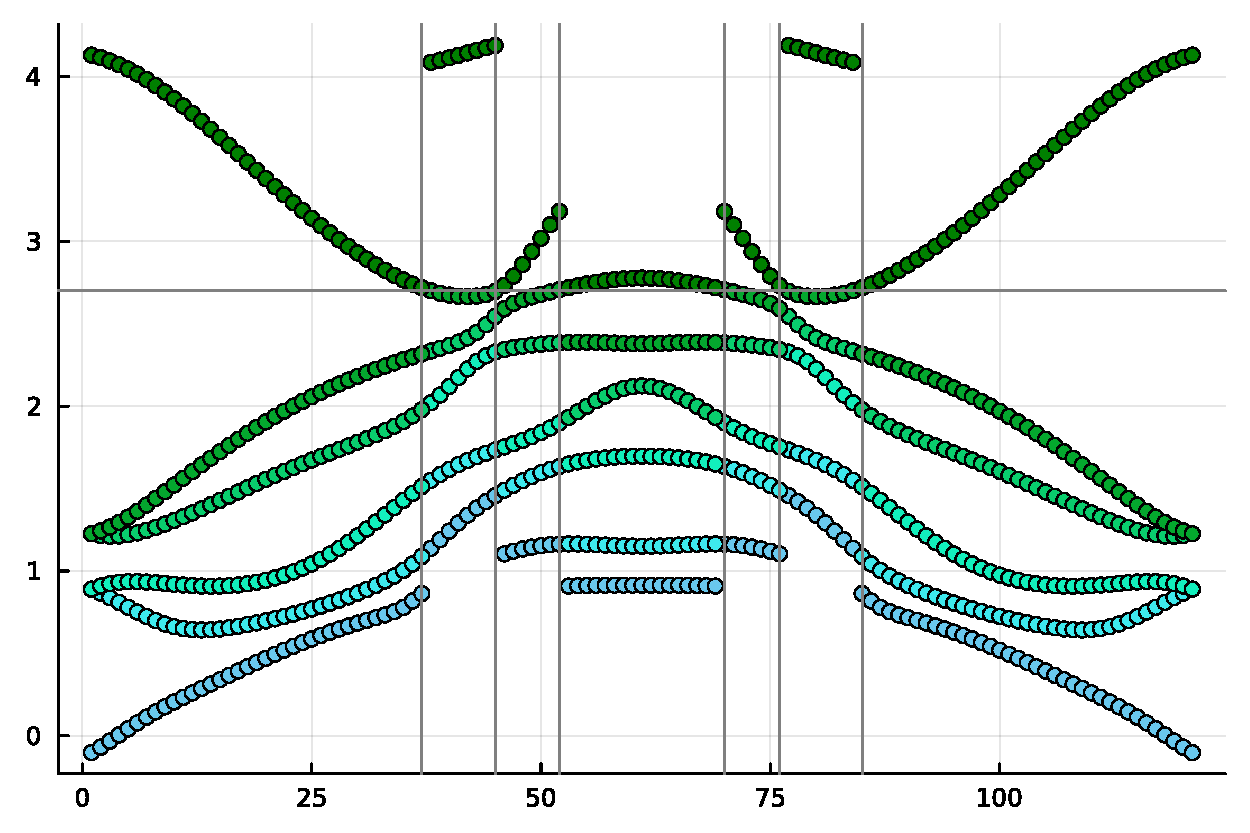
\includegraphics[width=0.5\textwidth]{plots/dft-level-bands.pdf}
    \caption{Example of how \shortcode{inteqp} misidentifies DFT-level bands:
    the data is from the DFT column of \shortcode{eqp.dat};
    the colors of points are about the band index.}
    \label{fig:inteqp-shuffle-band-index-1}
\end{figure}

If the system is metallic in the DFT level 
(regardless of what $GW$ says about the material, 
and the screening model used)
and \shortcode{inteqp} is used, 
this is expected:
somehow, \shortcode{inteqp} assumes the system is an insulator,
and thus states above the Fermi energy (but not too far from it)
has to be in one band.
Thus, if, say, the 120th band has more than one intersection points 
with the Fermi energy level,
its part below $\varphi_{\text{F}}$ will be recognized as the 119th band
in the eyes of \shortcode{inteqp}.
This can be seen by plotting the DFT column of the \shortcode{eqp.dat} output of \shortcode{inteqp}
(\prettyref{fig:inteqp-shuffle-band-index-1}).

Another type of band plot non-continuity is described in \cite{berger2020potential} 
and can be solved by COHSEX??? TODO

A further type of non-continuity comes from mistakenly linking a wrong \shortcode{epsmat.h5} 
or \shortcode{eps0mat.h5} file.
This sometimes displaces some segments of bands below a certain band index downwards or upwards.

\subsection{The size of band gap}\label{sec:band-gap-problem}

DFT is infamous for underestimating the band gap.

\begin{itemize}
    \item Use hybrid functionals like HSE.
    \item Let $GW$ correct the band structure. TODO: but how? How to avoid the error in \prettyref{sec:semimetal-error-1}?
\end{itemize}

\subsection{SOC effects are too strong}

When SOC effects are much stronger than expected: 
\begin{itemize}
    \item Are you using relativistic pseudopotentials for a non-SOC run?
        This is \emph{not} correct 
        (and unfortunately QuantumESPRESSO never tells us when this happens).
    \item TODO: 
\end{itemize}

\subsection{When we get a semimetal in the DFT step but it should be an insulator}\label{sec:unexpected-metal}

This is similar to \prettyref{sec:band-gap-problem}.

Note that naively feeding the semimetal result into BerkeleyGW 
while still using the insulator procedure
may result in errors in \prettyref{sec:segment-fault-1}. 

One way to solve the problem is 
to manually move the conduction bands and the valence bands away from each other.
Naively using the \shortcode{eqp_correction} option 
and shifting bands near the Fermi surface away from each other 
leads to \prettyref{sec:semimetal-error-1},
precisely because 
``QP corrections'' (i.e. the energy shift manually added by me) 
change the character of some states from valence to conduction.
The \shortcode{mf_header/kpoints/occ} and \shortcode{mf_header/kpoints/ifmax} datasets 
in the \shortcode{WFN.h5} file 
have to be modified accordingly.
A procedure to do so can be found \href{./scripts/wfn-editing/move-occupation.jl}{here}.
TODO: should this be done in \shortcode{2-sigma}?

The problem with this method is we don't have \shortcode{eqp_correction} in \shortcode{kernel}. TODO 

\subsection{The band plot seems reasonable but the band gap is strange}

When doing convergence tests, 
you may find changing a parameter 
somehow leads to a rather large change in the band gap. 
This may be because you accidentally use \shortcode{WFN} 
with \shortcode{number_bands} set for \shortcode{WFNo} 
in one of the instances. 
This essentially leads to an under-converged problem: 
suppose we have 200 bands in \shortcode{WFNo},
but there are 1000 bands in \shortcode{WFN}, 
and if we set \shortcode{number_bands} to \shortcode{200} 
while using \shortcode{WFN}, 
then of course the calculation is severely under-converged.

\subsection{The DOS curve is too smooth}

This usually can be solved by 
setting \shortcode{occupations} to \shortcode{tetrahedra}
in the \shortcode{bands} step,
and using a smaller \shortcode{degauss} in the \shortcode{projwfc} step.
Note that when doing so, 
the \shortcode{smearing} and \shortcode{degauss} options 
should not be set, 
or otherwise by default the calculation will be done with gaussian smearing.

\subsection{The Wannier-interpolated band structure looks weird}

\begin{itemize}
    \item A denser $\vb*{k}$-grid always improves the accuracy. 
\end{itemize}

\bibliographystyle{plain}
\bibliography{gw,dft,wannier,hubbard,quasiparticle,cohsex,structure,phonon,light-matter}

\end{document}